\phantomsection
\addcontentsline{toc}{chapter}{\textbf{Introduction en français}}
\onehalfspacing
\chapter*{Introduction en français }

L'humanité se trouve dans une ère écologique critique, où les seuils écologiques du système terrestre ont été franchis. La notion de "frontières planétaires" \citep{rockstrom2009safe,steffen_2015_planetary} illustre la façon dont l'anthroposphère, les effets des activités humaines à l'échelle de la planète, est devenue une composante fonctionnelle supplémentaire et est capable de modifier le système terrestre \citep{richardson_earth_2023} aux côtés de la géopshère (flux d'énergie et matériaux non vivants de la Terre et de l'atmosphère) et de la biosphère (tous les organismes vivants/écosystèmes). Le cadre des "limites planétaires" identifie les limites de l'impact de l'anthroposphère sur le système terrestre qui peuvent sauvegarder l'état interglaciaire de la Terre - le seul où la civilisation est connue - en identifiant un "espace opérationnel sûr". Parmi ces neuf limites, \cite{richardson_earth_2023} estime que six ont été franchies, menaçant la stabilité et la résilience du système terrestre. 

\begin{figure}[h]
	\centering
	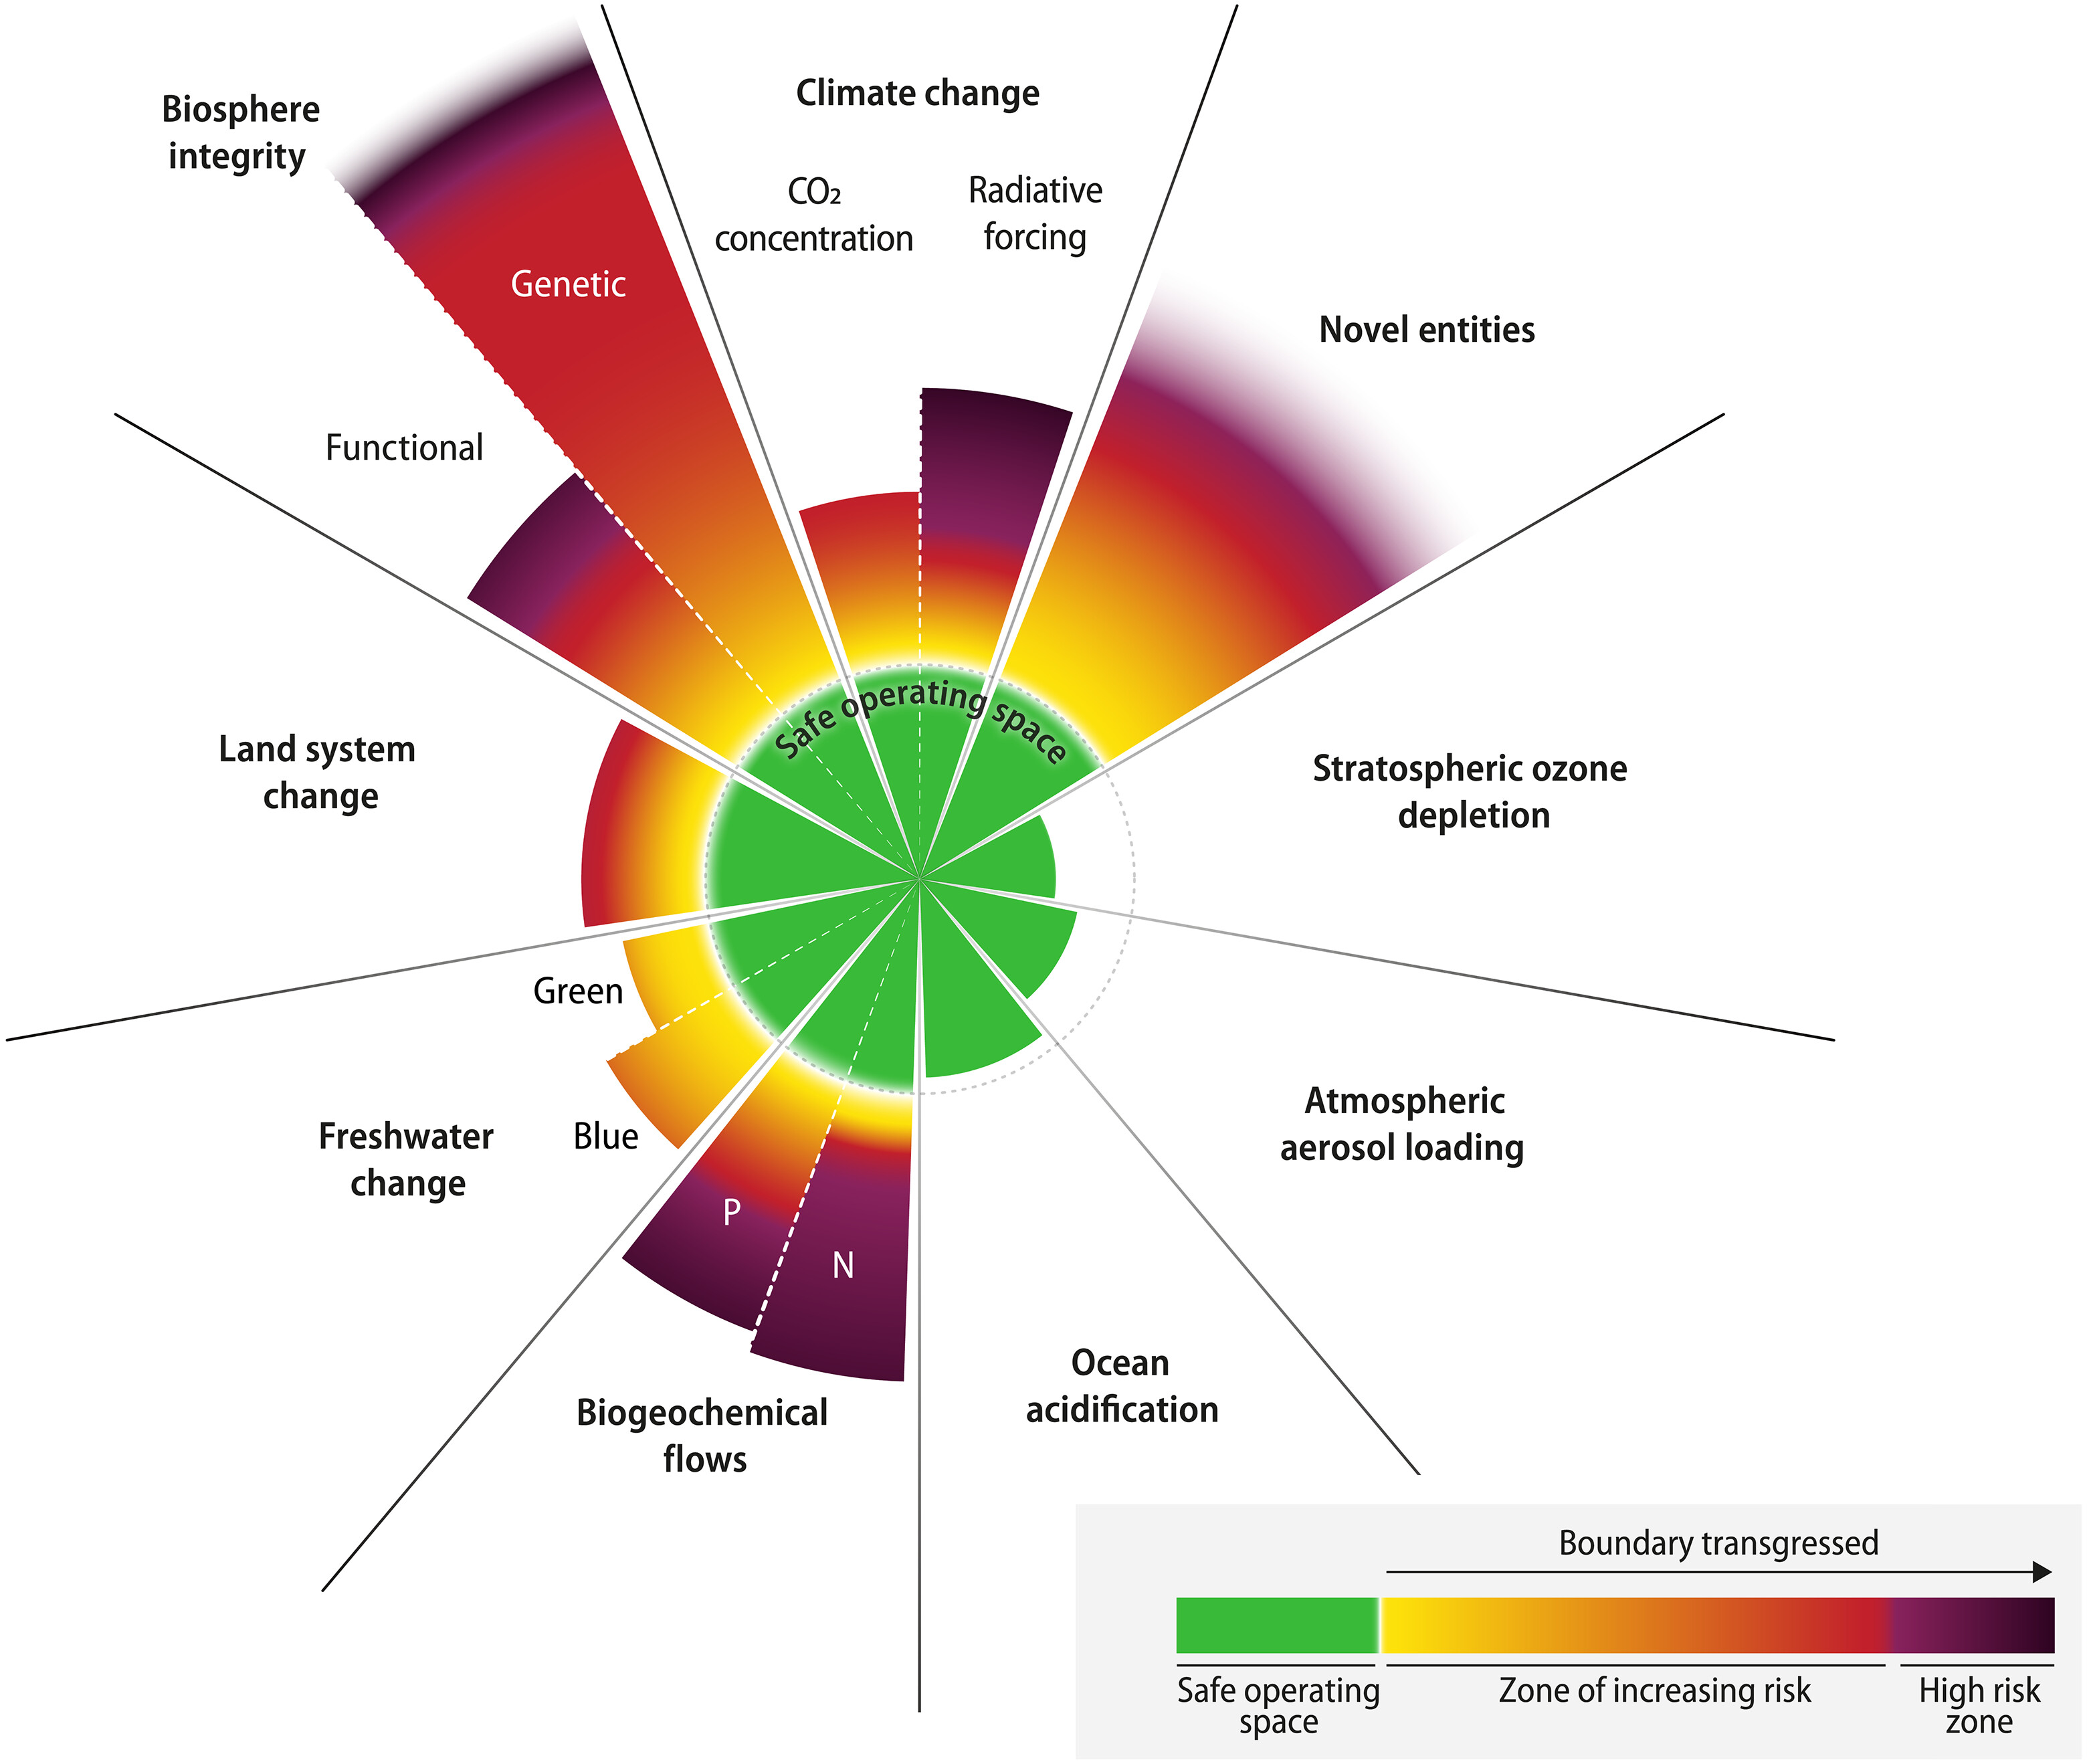
\includegraphics[width= .7\textwidth]{figures/intro/planetary_bounds.jpg}
	\caption{État actuel des variables de contrôle pour les neuf limites planétaires, à partir de \cite{richardson_earth_2023}}
\end{figure}

Parmi ces limites planétaires, l'intégrité de la biosphère a progressivement suscité un intérêt particulier, de même que son interaction avec d'autres limites, telles que le changement climatique, ou des entités nouvelles (par exemple, les polluants organiques synthétiques, les matières radioactives, la pollution microplastique...). Créé en 2012, le Groupe Interdisciplinaire sur la Biodiversité et les Services Ecosystémiques (IPBES\footnote{Interdisciplinary Panel on Biodiversity and Ecosystem Services}) a tiré la sonnette d'alarme sur l'état de la « nature » à l'échelle mondiale. Son président, Sir Robert Watson, l'a clairement exprimé\footnote{Voir le \href{https://www.ipbes.net/news/Media-Release-Global-Assessment}{communiqué de presse du rapport 2019}} :

\begin{displayquote}
\textit{Les preuves accablantes du Rapport d'Evaluation Global de l'\cite{ipbes_2022_6417333}, provenant d'un large éventail de domaines de connaissances, présentent un tableau inquiétant [...]. La santé des écosystèmes dont nous et d'autres espèces dépendons se détériore plus rapidement que jamais. Nous sommes en train d'éroder les fondements de nos économies, de nos moyens de subsistance, de notre sécurité alimentaire, de notre santé et de notre qualité de vie dans le monde entier}\footnote{Traduit par l'auteur}
\end{displayquote}

La « nature » est un concept central dans le cadre de l'IPBES \citep{ipbes_2022_6417333} :

\begin{displayquote} 
\textit{La nature (également définie comme la nature vivante) [est] le monde non humain, y compris les caractéristiques coproduites, avec un accent particulier sur les organismes vivants, leur diversité, leurs interactions entre eux et avec leur environnement abiotique. Dans le cadre des sciences naturelles, la nature comprend, par exemple, toutes les dimensions de la biodiversité, les espèces, les génotypes, les populations, les écosystèmes, la biosphère, le fonctionnement des écosystèmes, les communautés, les biomes, les systèmes de maintien de la vie sur Terre et leurs processus écologiques, évolutifs et biogéochimiques associés, ainsi que la diversité bioculturelle. Dans le cadre de l'économie, il comprend des catégories telles que les ressources naturelles biotiques, le capital naturel et les actifs naturels. Dans le contexte plus large des sciences sociales et humaines et des sciences environnementales interdisciplinaires, il est fait référence à des catégories telles que le patrimoine naturel, l'environnement vivant ou le non-humain. Dans le contexte d'autres systèmes de connaissance, il comprend des catégories telles que "Terre mère" [...], "Pachamama" [...]}.
\hspace*{\fill} \small{ \cite{ipbes_2022_6417333}, p.14, voir aussi \cite{DIAZ20151} }
\end{displayquote}

La nature, telle qu'elle est définie dans cette approche, est un objet très vaste et complexe. Elle se définit à travers des différences ontologiques et épistémiques (vivant et non-vivant), différents types d'interactions, à diverses échelles (génotypes v. écosystèmes), à différents types de processus (biologiques v. écologiques), et à travers différents champs d'investigation (sciences naturelles v. sciences sociales). Dans cette thèse, j'étudie plus spécifiquement la "biodiversité", qui se concentre sur la variabilité des organismes vivants. Bien qu'il s'agisse d'un concept ambigu, la biodiversité tend à mettre l'accent sur les organismes vivants, en relation avec leur environnement matériel, biotique et abiotique (par opposition à l'étude de l'environnement non vivant) et sur son rôle essentiel parmi les autres composantes du système terrestre.

Le rapport de l'\cite{ipbes_2022_6417333} documente les changements drastiques que subit la biosphère et examine ces changements dans une optique anthropocentrique, c'est-à-dire en médiatisant les changements susmentionnés par les contributions multiples et diverses que la nature et la biodiversité apportent à l'homme. Il souligne l'impact de leur perturbation sur la vie humaine et met en évidence le rôle des facteurs anthropogéniques (c'est-à-dire d'origine humaine) dans la perturbation de la nature et de la biodiversité. 
 
Ce rapport fixe différents objectifs à la recherche scientifique. Le premier objectif est d'expliquer les mécanismes de rétroaction : comment la vie de l'humanité influence-t-elle la biodiversité ? En réponse, comment la biodiversité influe-t-elle sur la vie de l'humanité ? Cet objectif implique, d'une part, de comprendre les causes et de mesurer les facteurs anthropiques directs et indirects de changement dans la nature et la biodiversité et, d'autre part, de comprendre les canaux et les échelles par lesquels la nature et la biodiversité contribuent aux moyens de subsistance de l'homme, ainsi que de mesurer ces contributions. Par conséquent, l'étude de la disparition de la nature et des possibilités d'y remédier nécessite une perspective intégrée, qui associe les sciences naturelles aux sciences sociales, par le biais de cadres tels que les systèmes socio-écologiques \citep{Ostrom2009} ou l'économie environnementale et écologique \citep{daly_ecological_2007}. 
\\
Le deuxième objectif est de fournir un cadre pour évaluer l'opportunité, la faisabilité et les moyens de mise en œuvre des voies collectives qui permettraient de remédier à la crise à laquelle la nature est confrontée. D'une certaine manière, il s'agit de concevoir et de mettre en œuvre des voies politiques vers des avenirs durables, c'est-à-dire de trouver des voies ou des méthodes d'action définies choisies parmi des alternatives, aux niveaux individuel, collectif ou gouvernemental, pour parvenir à des états futurs du monde qui restent dans un espace de fonctionnement sûr en ce qui concerne les limites planétaires \citep{rockstrom2009safe,steffen_2015_planetary}.

Dans cette thèse, j'aborde ces deux objectifs en utilisant un cadre issu de l'économie et de l'écologie. Une première version des questions de recherche que cette thèse vise à résoudre est la suivante : 

\begin{enumerate}
\item Quelles sont les relations de rétroaction entre la biodiversité et les facteurs anthropogéniques de son déclin ? 
\item Quels sont les mécanismes sous-jacents auxquels les politiques doivent s'attaquer pour remédier à ce déclin ?
\item Comment les approches économiques et écologiques intégrées peuvent-elles être utilisées et affinées pour analyser, informer et concevoir des politiques publiques? 
\end{enumerate}

Afin d'affiner ces questions, je commence par définir le concept de biodiversité, à travers ses évaluations en sciences naturelles et sociales, et je souligne les tendances actuelles de sa disparition.

\phantomsection
\addcontentsline{toc}{section}{Emergence et définition de la biodiversité comme concept écologique}
\subsection*{Emergence et définition de la biodiversité comme concept écologique }


La biodiversité est apparue en tant que concept dans les années 1980, parallèlement à l'émergence de la "biologie de la conservation", une branche de la biologie qui s'intéresse à la protection de la "diversité biologique" \citep{soule_what_1985}, en réponse à l'accélération de la disparition des espèces. La position morale de la biologie de la conservation est que les espèces doivent être protégées pour elles-mêmes \citep{soule_conservation_1986}, elles ont une valeur intrinsèque. 
Le concept de biodiversité s'inscrit donc dans un jugement éthique et un appel à l'action. Dans le sillage de la conférence des Nations unies sur l'environnement et le développement qui s'est tenue à Rio en 1992, la \href{https://www.cbd.int/}{Convention sur la diversité biologique} s'est imposée comme un traité international visant à sauvegarder la biodiversité. Ce faisant, elle a fourni une définition internationalement reconnue :

\begin{displayquote}
\textit{La "diversité biologique" désigne la variabilité des organismes vivants de toute origine y compris, entre autres, les écosystèmes terrestres, marins et autres écosystèmes aquatiques et les complexes écologiques dont ils font partie ; cela comprend la diversité au sein des espèces et entre espèces ainsi que celle des écosystèmes.}\\
\hspace*{\fill} \small{\href{https://www.cbd.int/convention/articles/default.shtml?a=cbd-02}{Article 2 de la Convention sur la Diversité Biologique}}\footnote{Traduit par l'auteur}
\end{displayquote}

Cette définition met en évidence un élément clé de différenciation par rapport à d'autres parties de la nature, à savoir la nature vivante des objets étudiés. Par rapport aux facteurs abiotiques, la diversité biologique se caractérise par une croissance, une reproduction et un métabolisme intrinsèques (au niveau de l'individu et de la population), ainsi que par une évolution (au niveau de la génétique et de l'espèce). En outre, ces taux de changement dans le temps sont commensurables avec l'expérience humaine, et la plupart des processus (par exemple, la reproduction, l'effondrement ou la reconstitution des populations, l'évolution génétique) peuvent être observés au cours d'une vie humaine, par opposition à l'échelle temporelle géologique. 

Comme le soulignent \cite{VanDyke2008} et \cite{mouysset_diversity_2023}, la définition de la biodiversité est difficile, car elle recouvre des dimensions éthiques, conceptuelles et de mesure. La biodiversité peut être considérée comme "une qualité intrinsèque et sans mesure des systèmes naturels qui devrait être préservée pour elle-même" \citep{VanDyke2008, mouysset_diversity_2023}\footnote{Traduction de l'auteur}, mais elle se réfère également à des caractéristiques mesurables.
%
Cette définition implique différentes échelles d'un point de vue hiérarchique, au niveau génétique, au niveau de l'espèce, de la communauté et de l'écosystème (défini comme l'interaction des communautés et de leur environnement abiotique). Ces niveaux impliquent différentes formes de mesure, notamment la distribution des gènes, l'abondance des espèces (le nombre d'individus dans une population, à un moment et à un endroit donnés), la richesse des espèces (le nombre d'espèces différentes, à un moment et à un endroit donnés) au sein des communautés, entre les communautés et à des échelles plus grandes (les diversités alpha, bêta et gamma), ainsi que les variations des facteurs abiotiques qui forment les écosystèmes, tels que la température, l'humidité, la qualité de l'eau, la qualité du sol, etc. 
Elle comprend également différents types de diversité : la diversité structurelle (par exemple, les couches de la canopée dans les forêts, le sex-ratio dans les populations animales), la diversité de composition (la variété et l'abondance des espèces au sein d'une communauté) et la diversité fonctionnelle (la variété des processus environnementaux réalisés par les organismes vivants dans une zone donnée, par exemple la séquestration du carbone, le cycle des nutriments ou la dispersion des graines, voir \cite{loreau_biodiversity_2002}).

\begin{figure}
	\centering
	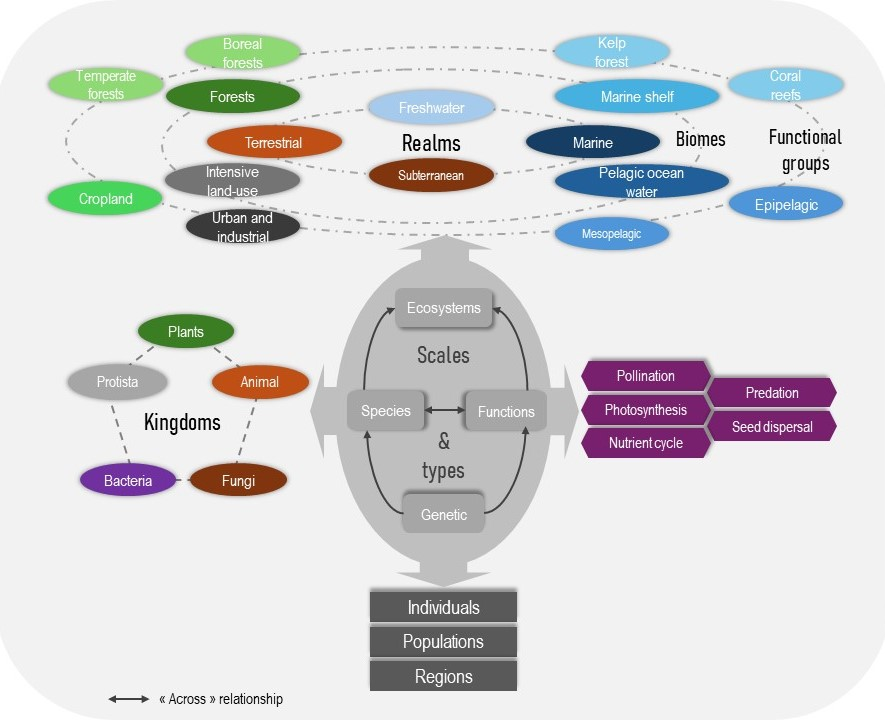
\includegraphics[width =.8\textwidth]{figures/intro/biodiv_illustration.jpg}
	\caption{ La biodiversité : un concept multiforme à travers échelles et types}
	\label{fig:intro_biod_french}
\end{figure}

\cite{mouysset_diversity_2023} souligne la difficulté d'articuler la définition avec les niveaux communs de l'analyse scientifique, par exemple génétique, taxonomique et écosystémique, car le niveau de biodiversité peut se situer entre les deux : "les populations peuvent être considérées d'un point de vue génétique et taxonomique, ou les communautés qui se situent entre les niveaux taxonomique et écosystémique". En outre, la diversité structurelle et compositionnelle pouvant être considérées comme les sources de la diversité fonctionnelle, il peut être difficile de travailler avec les différentes classes de diversité en raison de leur colinéarité. 

Les multiples dimensions de la biodiversité mettent en évidence plusieurs de ses caractéristiques essentielles. Tout d'abord, il est impossible de mesurer la biodiversité à l'aide d'un seul indicateur. L'étude de la biodiversité nécessite de multiples indicateurs pour évaluer de manière intégrée l'évolution de la biodiversité, à toutes les échelles et pour tous les types de diversité. L'émergence du concept répond à un désir de protéger la biodiversité pour son propre bien, mais aussi pour celui de l'humanité. 


\phantomsection
\addcontentsline{toc}{section}{Les Contributions de la Nature  aux Populations : logiques de conservation de la biodiversité}
\subsection*{Les Contributions de la Nature aux Populations : logiques de conservation de la biodiversité}

D'abord descriptives, les fonctions des écosystèmes ont été de plus en plus considérées d'un point de vue humain à partir des années 1970 \citep{hueting1969functions, schumacher1973small}, évoluant vers le concept de services écosystémiques \citep{ehrlich1981extinction} pour illustrer les conséquences de la perte de biodiversité \citep{gomez_history_2010}. Cette évolution a marqué le passage d'une valeur intrinsèque à une valeur anthropocentrique (c'est-à-dire donnée par l'homme) \citep{mouysset_diversity_2023}, reconnaissant les valeurs instrumentales et relationnelles de la biodiversité - servir les objectifs des humains et favoriser des relations significatives avec les autres et l'environnement. Progressivement, la biodiversité a dû être protégée pour son rôle dans le maintien de la vie humaine.

Le concept a fait son chemin dans la recherche universitaire, et lorsque \cite{Costanza1997} a quantifié la valeur du capital naturel et des services écosystémiques au stupéfiant montant de 33 trillions \$USD, soit environ 30\% du PIB mondial de 2020, le concept est entré dans l'arène politique. En 2005, le Millenium Ecosystem Assessment \citep{MEA2005} a placé les services écosystémiques au centre de l'agenda politique : elle a souligné une valeur anthropocentrique des services écosystémiques, mais a établi une dépendance des sociétés humaines aux services écosystémiques, et plus loin, au fonctionnement de l'écosystème. À cet égard, le Millenium Ecosystem Assessment \citep{MEA2005} a marqué un tournant dans la sauvegarde de la biodiversité par le biais d'un paradigme de soutenabilité forte (voir encadré 1), et a déclenché l'opérationnalisation du concept dans les politiques à grande échelle (ce que je développerai plus loin). Le cadre des services écosystémiques a été divisé en 4 catégories, liées au type spécifique de services contribuant au "bien-être humain" : les services de soutien (par exemple, les services permettant à d'autres services écosystémiques d'être présents, y compris le cycle des nutriments et la production primaire) et les services de régulation ("avantages obtenus par la régulation des processus écosystémiques", par exemple la pollinisation, la décomposition des déchets, la gestion de l'eau, etc.) ; les services culturels ("les avantages non matériels que les gens tirent des écosystèmes par l'enrichissement spirituel, le développement cognitif") et les services d'approvisionnement ("tous les produits tirés des écosystèmes",\cite{MEA2005}, p.54)

\begin{figure}[h]
	\centering
	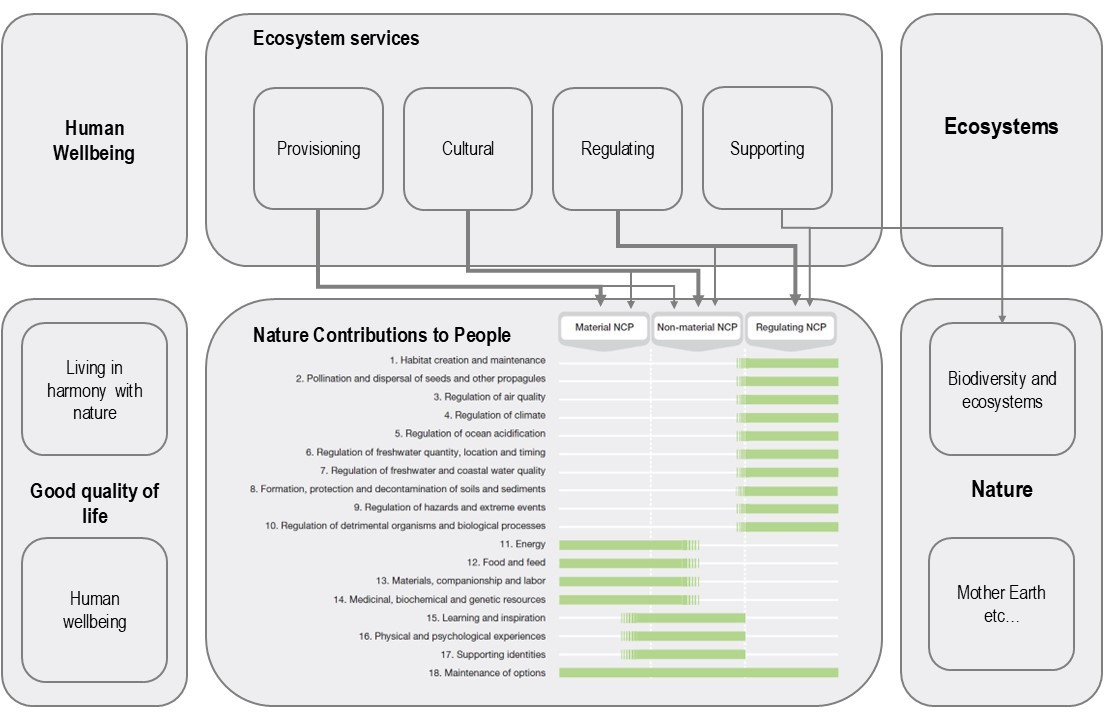
\includegraphics[width = \textwidth]{figures/intro/NCPs2.jpg}
	\caption{Description des 18 Contributions de la Nature aux Populations et du lien entre le cadre des CNP \citep{ipbes_2022_6417333} et le cadre des services écosystémiques \citep{millennium2005ecosystems}}
	\subcaption*{Adapté depuis \cite{diaz_2018} et \cite{ipbes_2022_6417333}}
\end{figure}

Récemment, l'IPBES est passée à un nouveau cadre conceptuel mettant en évidence les contributions de la nature aux populations (CNP) \citep{DIAZ20151}, définies comme "toutes les contributions, positives et négatives, de la nature vivante [...] à la qualité de vie des populations" \citep{diaz_2018}. Ce cadre sous-tend trois types de contributions aux personnes : les contributions matérielles aux personnes (flux de la nature vers les personnes généralement consommés pour "faire fonctionner une société ou une entreprise" \cite{ipbes_2022_6417333}, p.16), les contributions non matérielles (par exemple, les effets de la nature sur "les aspects subjectifs et psychologiques qui sous-tendent la qualité de vie des populations") et les contributions régulatrices (par exemple, "les aspects fonctionnels et structurels des organismes et des écosystèmes qui modifient les conditions environnementales vécues par les personnes et/ou régulent la génération de contributions matérielles et non matérielles"). Ce cadre met en évidence le fait que les contributions de la nature à l'homme peuvent être positives ou négatives et dépendent de la définition spatiale et temporelle de la contribution, puisqu'une entité donnée peut être à la fois la source de contributions positives et négatives : par exemple, les forêts favorisent l'habitat, mais risquent également de mettre en danger les personnes en cas d'incendies de forêt. En outre, elle offre une vision plus globale que les services écosystémiques, car elle englobe des perspectives allant de la biodiversité en tant que capital naturel utilisé dans une fonction de production écologique (voir \cite{polasky_integrating_2009} pour une revue), ainsi que des perspectives où la biodiversité a une agence et est liée par des obligations de soins réciproques envers les humains \citep{descola}. 

Une correspondance à multiples facettes entre les différentes composantes et dimensions de la biodiversité et ses contributions à l'homme est à la base des moyens de subsistance de l'homme. Le déclin mondial de la biodiversité menace les CNP.

\clearpage
\begin{tcolorbox}[breakable,  
colback=verylightgray, 
colframe=gray!75!black, 
title= {Box 1 - Soutenabilité Faible et Forte},
fontupper=\small]

\par % This \par ensures spacing before the text starts
\justifying % Start justified text

En 1987, la publication du rapport Brundtland \citep{brundtland} a donné une définition large du développement durable : 

\begin{displayquote}
\textit{Par essence, le développement durable est un processus de changement dans lequel l'exploitation des ressources, la direction des investissements, l'orientation du développement technologique et les changements institutionnels sont tous en harmonie et améliorent le potentiel actuel et futur de satisfaction des besoins et des aspirations de l'humanité}\footnote{Traduit par l'auteur}\\
\hspace*{\fill}\small{\cite{brundtland}, p.43}
\end{displayquote}

La mise en œuvre du développement durable est restée une question ouverte. En économie, une « perspective de durabilité faible », inaugurée par les travaux de \cite{hartwick_intergenerational_1977} et \cite{solow_intergenerational_1986} sur les ressources épuisables, suggérait que « le maintien d'un stock de capital non décroissant, qui pourrait être mis en pratique en investissant dans le capital manufacturé toutes les rentes dérivées de l'exploitation des ressources naturelles non renouvelables »\footnote{Traduit par l'auteur} \citep{gomez_history_2010} était suffisant pour maintenir la consommation au fil du temps. Dans cette approche, le capital naturel pouvait être intégralement remplacé par le capital humain. D'autre part, l'approche de la « durabilité forte » prône la complémentarité, plutôt que la substituabilité, des ressources naturelles \citep{costanza_daly}, reconnaissant ainsi la dépendance des humains à l'égard des écosystèmes.
\end{tcolorbox}

\phantomsection
\addcontentsline{toc}{section}{Déclin de la biodiversité : tendances et facteurs}
\subsection*{Déclin de la biodiversité : tendances et facteurs}

Les mesures de la biodiversité diminuent à toutes les échelles d'analyse. Les conditions structurelles des écosystèmes, la composition des communautés écologiques et les populations d'espèces ont connu des changements spectaculaires.
La part des habitats sauvages protégés et inchangés s'est effondrée sur terre et en mer \citep{watson_2016_catastrophic, jones_2018_location} pour atteindre 23\% et 12\% de l'espace, respectivement. Au niveau des communautés, la part de la biodiversité initialement présente tombe en dessous de 90 \% dans tous les biomes, \citep{Hill311787} et les communautés locales deviennent de plus en plus semblables \citep{mckinney_1999_biotic}, sous l'effet de l'augmentation de l'étendue des espèces exotiques envahissantes animales et végétales, en hausse de 13 \% par décennie \citep{seebens_no_2017}. A\` ce jour, la richesse des espèces mondiales est menacée par une extinction massive, car le taux mondial d'extinction des espèces est au moins dix fois plus élevé que le taux moyen des 10 derniers millions d'années et s'accélère \citep{barnosky_has_2011, ceballos_accelerated_2015}. En moyenne, 25 \% des espèces sont actuellement menacées d'extinction à l'échelle mondiale dans un large éventail d'espèces végétales et animales, sur terre et en mer \citep{IUCN_redlist_2024}. En utilisant des méthodes fondées sur l'habitat, \cite{Hoskins309377}\footnote{La liste rouge de l'UICN utilise des comptes détaillés pour les espèces, dans une approche ascendante, afin d'analyser le risque d'extinction des espèces. Une approche descendante, qui s'appuie sur l'évolution de l'habitat disponible et la relation espèce-zone, utilise les changements dans l'utilisation des terres pour prévoir l'extinction des espèces de manière plus globale. \citep{Diamond1972BiogeographicKE}} constatent que des centaines de milliers d'espèces végétales et animales sont menacées et rembourseront la \textit{dette d'extinction} causée par les changements anthropogéniques de leurs habitats : seulement 92.1\% des espèces de vertébrés terrestres, 91,6\% des invertébrés terrestres et 90,7\% des plantes terrestres disposent d'un habitat suffisant pour subsister. Ces résultats suggèrent qu'environ un demi-million d'espèces animales et végétales terrestres - dont plus de 3 000 vertébrés et plus de 40 000 plantes - sont condamnées à s'éteindre, à moins que leurs habitats ne s'améliorent à temps pour l'empêcher \citep{ipbes_2022_6417333}.

Les facteurs de déclin de la biodiversité sont d'origine anthropique. Ils peuvent être classés en deux catégories : les facteurs \textit{directs}, qui découlent directement des actions humaines, comme le changement d'utilisation des terres, le changement climatique anthropique, la surexploitation, et les facteurs \textit{indirects}, qui peuvent être considérés comme la cause première des facteurs directs, comme les changements dans les systèmes de valeurs qui sous-tendent les utilisations de la nature (\cite{ipbes_2022_6417333} p. 55), la démographie (urbanisation et migration), la technologie, l'économie (transitions sectorielles, expansion du commerce) et la gouvernance (y compris les systèmes de risque pour l'accès aux ressources).

Une synthèse des sciences naturelles réalisée par l'\cite{ipbes_2022_6417333} souligne le rôle des principaux facteurs à l'échelle mondiale et dans tous les biomes (voir figure \ref{fig:intro_impacts_french}).
Il montre que le changement d'utilisation des terres et des mers, c'est à dire la perte, la fragmentation, et la dégradation de  l'habitat\footnote{La perte d'habitat est sans aucun doute le principal moteur du déclin de la biodiversité terrestre. Les effets de la fragmentation sur la biodiversité sont très controversés. D'un point de vue théorique, des modèles ont été développés pour étudier l'évolution des populations et des communautés dans l'espace et le temps, par exemple les modèles de métapopulation et de métacommunauté. Les connaissances théoriques soulignent que la fragmentation de l'habitat augmente le risque d'extinction et réduit la probabilité de colonisation, ce qui se traduit par une baisse de la survie et de la diversité \citep{adler_persistence_1994,hill_habitat_1999, thompson_loss_2017}. À l'échelle communautaire, l'augmentation de la diversité entre les communautés (par exemple, la diversité bêta) peut résulter des différentes exigences des espèces en matière de ressources et de la plus grande étendue spatiale, qui englobe donc une plus grande hétérogénéité environnementale, résultant de la fragmentation \citep{lasky_reserve_2013, chisholm_species_2018}. Toutefois, ces effets s'atténuent à mesure que la perte d'habitat diminue.   Au niveau empirique, l'effet de la fragmentation est très discuté. Selon \cite{fahrig_ecological_2017}, il n'existe aucune preuve empirique qu'un groupe de petites parcelles d'habitat a généralement une valeur écologique inférieure à celle de grandes parcelles de la même superficie totale. Des éléments montrent toutefois que la fragmentation ne réduit pas la connectivité des habitats, car la connectivité fonctionnelle est améliorée (par exemple, les espèces sont en contact avec un plus grand nombre de parcelles de ressources différentes, ce qui améliore le fonctionnement global des écosystèmes). Le débat entre \cite{fletcher_is_2018} et \cite{fahrig_habitat_2019} porte sur les critiques fondées sur la capacité des modèles statistiques à englober l'effet de la fragmentation en cas de perte d'habitat \citep{ruffell_accounting_2016}. En outre, il reflète la difficulté de l'écologie paysagère, car différents mécanismes à travers les échelles, par exemple la parcelle, le paysage et la région d'étude, et des mesures, telles que la taille de la parcelle, l'isolement de la parcelle (par exemple la distance entre les parcelles) et la distance au bord de la parcelle (par exemple la distance au bord à l'intérieur de la parcelle) interagissent avec des interactions non linéaires possibles.}
\%
L'exploitation directe de la faune et de la flore sauvages et la dégradation de l'habitat de la faune sont responsables de 30\% des impacts sur la biodiversité. L'exploitation directe de la faune et de la flore sauvage représente 23 \% des impacts. Le changement climatique, qui se traduit par des modifications des conditions biogéographiques et des changements d'habitat, a un impact sur les caractéristiques des espèces et l'évolution génétique, ce qui représente 14\% des impacts, et la pollution représente 14\% des impacts. Enfin, les espèces exotiques envahissantes représentent 11\%. Ces facteurs ont des impacts différents selon les écosystèmes et les biomes \citep{ipbes_2022_6417333}. 

\begin{figure}[h]
	\centering
	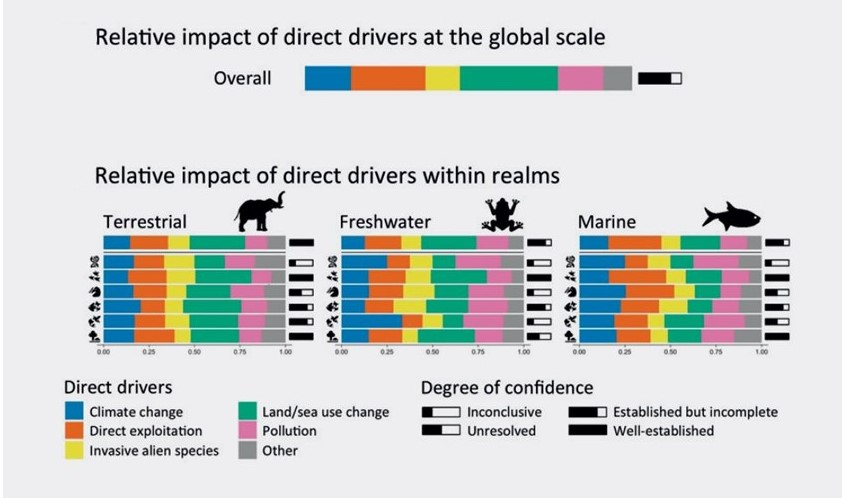
\includegraphics[width = .95 \textwidth]{figures/intro/intro_impactsfin.jpg}
	\caption{Effets aggrégés et par biômes des impacts des moteurs anthropogéniques directs du déclin de la biodiversité, adapté de  \cite{ipbes_2022_6417333}}
	\label{fig:intro_impacts_french}
\end{figure}

Sur terre, le changement d'usage des terres est le facteur le plus important (30,5\%), sous l'effet de la déforestation et de l'agriculture, suivi de l'exploitation directe (21\%).  Les forêts tropicales et subtropicales sèches et humides abritent la plus grande diversité biologique. Par exemple, elles abritent les 10 hotspots qui comptent le plus grand nombre de vertébrés \citep{mittermeier_global_2011}. Dans ces forêts, la perte et la dégradation de l'habitat sont les principaux facteurs de réduction de l'abondance et de la richesse des espèces \citep{newbold_global_2014}. L' exploitation forestière sélective légale et illégale détruit l'habitat \citep{hoare2022establishing, bousfield_2023_large} et est combinée à la chasse et au braconnage des espèces sauvages \citep{gallego_2020_combined}, générant entre 60 et 180 milliards \$ USD de revenus \citep{gfi_2017}\footnote{Le commerce illégal d'espèces sauvages représente entre 5 et 23 milliards \$USD, tandis que l'exploitation forestière illégale représente entre 52 et 157 milliards \$USD}. 

Pour les espèces marines, la surexploitation est le principal moteur (29\%) \citep{ipbes_2022_6417333}. Avec 90 millions de tonnes de captures (et 141 milliards de dollars) en 2020 \citep{fao_2022_state}, les stocks halieutiques se situant à des niveaux biologiquement durables ont diminué pour atteindre 64,6\% en 2019, contre 90\% en 1974\footnote{Dans ce calcul, tous les stocks halieutiques sont pris en compte de la même manière, indépendamment de leur abondance ou de leurs captures}, sous l'effet de la surpêche dans le Pacifique Sud-Est et dans les mers Méditerranée et Noire. Néanmoins, la pêche illicite, non déclarée et non réglementée (INN) constitue une menace pour les pêcheries.  Selon des estimations datant d'il y a 15 ans \citep{agnew_estimating_2009} , elle représenterait entre 11 et 26 millions de tonnes de poisson pour une valeur de 10 à 23 milliards de dollars américains. 

En outre, le changement climatique anthropique entraîne des perturbations des écosystèmes sur terre \citep{burrell_anthropogenic_2020, conradi_reassessment_2024} et en mer \citep{gomes_marine_2024}, par le biais de changements dans divers canaux , y compris l'adéquation des habitats et les perturbations du réseau trophique. Sur terre, par exemple, les forêts, bois et maquis méditerranéens, qui couvrent 4 millions de km$^2$, sont des zones d'une diversité exceptionnellement élevée \citep{Mooney2001, blondel_2010}, menacées par l'expansion urbaine et l'augmentation du risque d'incendie de forêt.   La fréquence et la gravité des incendies de forêt devraient augmenter avec le réchauffement climatique \citep{Dupuy2019ClimateCI}, entraînant d'importants coûts directs et indirects pour la société , notamment la destruction d'infrastructures et des perturbations de l'activité économique \citep{wang_economic_2021}, les problèmes de santé liés à lafumée \citep{burke_wildfire_2023, heft-neal_behavior_2023}, la perturbation des caractéristiques structurelles des écosystèmes \citep{Ayars2023} et la menace pour la diversité biologique \citep{Wintle2020}.

\phantomsection
\addcontentsline{toc}{section}{Défis économiques des facteurs anthropogéniques du déclin de la biodiversité}
\subsection*{Défis économiques des facteurs anthropogéniques du déclin de la biodiversité}


La perte d'habitat et la surexploitation présentent des défis à la fois communs et différenciés.   Une cause commune identifiable est le coût d'opportunité élevé de la préservation de l'habitat ou de l'existence d'une espèce, en présence d'autres alternatives économiques pour la terre et le temps, ainsi que de contraintes financières. En outre, la perte d'habitat et la surexploitation partagent un aspect dynamique temporel, où les actions immédiates ont des conséquences durables, voire irréversibles.

La perte et la fragmentation de l'habitat dans les écosystèmes terrestres posent des problèmes spécifiques. Les forêts, par exemple, ont des usages multiples (ou CNP) pour différents agents : les bûcherons tirent profit du bois, certains défrichent les terres pour l'agriculture, les randonneurs recherchent des paysages vierges et les défenseurs de l'environnement visent à rétablir les cycles naturels. Les forêts ont également une valeur spirituelle et culturelle. Ces différents usages rentrent donc en conflit. Par exemple, la déforestation et l'urbanisation détruisent à la fois l'habitat et les terres sacrées, mais créent une valeur économique mesurée \citep{giglio_economics_2024}, tandis que la prévention des incendies de forêt peut endommager l'habitat des espèces sauvages \citep{bradshaw2018}. Les espèces peuvent également avoir des impacts mixtes ; les cerfs, par exemple, sont appréciés à faible densité mais causent des dommages à des densités plus élevées \citep{putman_identifying_2011}. Le changement climatique aggrave la perte d'habitat en modifiant la distribution des habitats et en augmentant les menaces telles que les incendies de forêt \citep{Dupuy2019ClimateCI,wasserman_climate_2023}.
    Une deuxième caractéristique essentielle pour mettre fin à la fragmentation des habitats est la prise en compte de l'ensemble des interdépendances, des retombées écologiques et des externalités économiques qui sous-tendent la dimension spatiale. La configuration de l'espace et le mouvement des espèces sont, au moins en partie, le résultat d'une décision économique. Le maintien de la connectivité des habitats passe par l'identification des parcelles et des chemins à conserver ou à restaurer qui y contribuent le plus, sous forme de corridors, d'écoducs ou de tremplins \citep{Turner2005, Turner2011}. La valeur des parcelles et des chemins pour la connectivité est intrinsèquement liée à leur environnement : au même endroit géographique, une parcelle a une valeur différente pour l'habitat de la biodiversité si elle est connectée à d'autres, ou si elle est isolée (voir encadré 2). Lorsque les chemins échappent au contrôle de l'homme, les parcelles ont une importance différente en fonction de leur emplacement, et lorsque l'emplacement des parcelles est fixe, l'étendue des chemins et leur emplacement sont primordiaux.
\\
Troisièmement, lorsque des actions et des utilisations multiples structurent des éléments connectés des écosystèmes (par exemple, différentes étendues de terre ou différentes échelles de biodiversité), elles entraînent des retombées spatiales, c'est-à-dire des conséquences qui vont au-delà de leurs effets \textit{in situ}, avec des répercussions dnas la durée. Lorsque ces retombées ne sont pas prises en compte par les agents qui les génèrent, elles peuvent être appelées « externalités spatiales dynamiques » \citep{sanchirico_bioeconomics_1999, costello_optimal_2008, costello_private_2017}. Étant donné que l'arrêt de la perte et de la fragmentation des habitats implique la conservation de parcelles de terre, les parties voisines peuvent très bien bénéficier (ou souffrir) d'un plus grand nombre d'espèces sauvages et de (dis-)services écosystémiques sur leur propriété, au fil du temps. Comme les agents réagissent aux profils d'action des autres, ils adoptent un comportement stratégique, à la fois dans l'espace et dans le temps. Ces externalités peuvent déclencher des problèmes spécifiques de "cercle vicieux" \citep{costello_private_2017} : lorsque les parties voisines d'un décideur qui entreprend la conservation, ou la réduction des risques, ne se rendent pas la pareille alors qu'elles bénéficient des retombées, un cercle vicieux de moindre action est déclenché. Inversement, lorsque les retombées écologiques sont positives, cela peut conduire tout le monde à utiliser une ressource à des niveaux non durables, même en présence de droits bien définis, en l'absence d'autres mécanismes \citep{janmaat_sharing_2005,kaffine_unitization_2010}.  Par conséquent, la fragmentation de l'habitat et la surexploitation sont liées par la connectivité spatiale. 
\\
Quatrièmement, arrêter la perte et la fragmentation des habitats implique de coordonner de nombreux acteurs en vue d'accroître la superficie et la connectivité des habitats, tout en tenant compte des coûts et des avantages associés, ainsi que des différents intérêts.
Dans certains cas, les contraintes financières, l'ampleur des coûts associés à l'augmentation de la connectivité des habitats et la difficulté de la coordination justifient une politique publique dans laquelle un planificateur central entreprend l'action \citep{Mouysset2012}. D'autre part, il existe des mécanismes permettant de décentraliser une planification spatiale efficace, qui peuvent être efficaces lorsque les coûts de coopération sont limités \citep{costello_private_2017, bareille_agglomeration_2023}. 

Pour mettre un terme à la surexploitation, il faut comprendre et traiter ses motivations. La surexploitation (ou le sous-contrôle, pour les espèces nuisibles) résulte d'un déséquilibre entre l'appropriation et l'utilisation des contributions de la nature aux populations (tant positives que négatives) et le niveau et la répartition socialement souhaitables de ces contributions, ainsi que du comportement stratégique non coordonné des agents. La nature commune de la plupart des ressources naturelles \citep{Gordon1954, smith_models_1969} a longtemps été identifiée comme l'une des principales raisons de leur disparition : de nombreux événements ont montré eux aussi des dynamiques de cercles vicieux, de tragédie des communs \citep{hardin_tragedy_1968}, où l'absence de droits de propriété sûrs a accéléré la surexploitation et le déclin des populations. Cette question est depuis longtemps au centre de l'attention, et les mécanismes reposant sur l'attribution de droits de propriété ont fait l'objet d'études approfondies \citep{libecap_tragedy_2009, costello_partial_2015, isaksen_tragedy_2019}.

\clearpage
\begin{tcolorbox}[breakable, 
colback =verylightgray, 
colframe=gray!75!black,
title={Encadré 2 - Habitat : perte, fragmentation et connectivité},
fontupper=\small]
\par 
\justifying

La perte d'habitat correspond à la perte de zones présentant des conditions environnementales adéquates pour la survie et le développement des espèces. À surface d'habitat constante, la fragmentation se traduit par une augmentation du nombre de parcelles et une diminution de la taille moyenne de chaque parcelle, comme le montre la figure \ref{fig:connectivity_intro_french}. 

La connectivité du paysage est définie par rapport à la fragmentation. Elle mesure "le degré auquel le paysage facilite ou entrave le mouvement entre les parcelles de ressources" \citep{taylor_connectivity_1993}. 
Elle recouvre une dimension \textit{structurelle}, qui décrit les arrangements physiques entre les parcelles, et une dimension \textit{fonctionnelle}, qui met l'accent sur la capacité et la réalisation des mouvements des individus à travers le paysage. Les mesures de connectivité globale tiennent compte du rôle des parcelles et des chemins différenciés. Dans le panneau D de la figure \ref{fig:connectivity_intro}, les parcelles encerclées jouent un rôle déterminant dans le maintien de la connectivité. Les parcelles d'habitat 1 et 2 ont le même nombre de parcelles connectées. Cependant, la parcelle 1 maintient la connexion entre les parcelles d'habitat situées à l'est et à l'ouest du paysage et est reliée à des parcelles fortement connectées. La suppression des parcelles d'habitat 1 et 2 aurait des conséquences plus importantes sur l'habitat que la suppression d'autres parcelles de taille identique. De même, la suppression du chemin en pointillé (en bas à gauche du panneau D) isolerait la parcelle 3, tandis que la suppression du chemin en pointillé ne laisserait pas la parcelle 4 isolée. Par conséquent, les chemins et les îlots ont des impacts différents sur la connectivité, en fonction des îlots et des chemins environnants.

\begin{center}
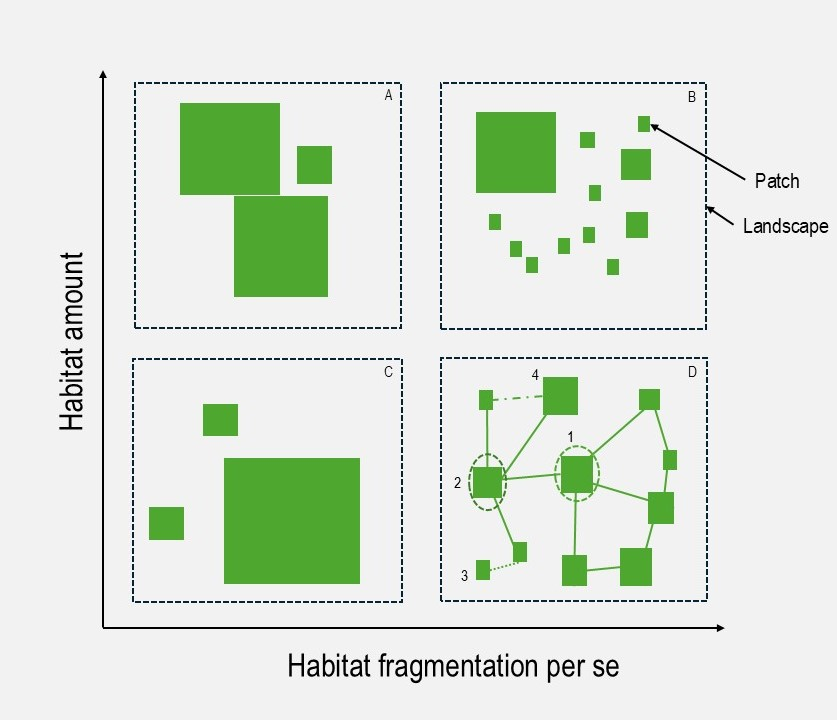
\includegraphics[width = .8\textwidth]{figures/intro/fragmentation.jpg}
\captionof{figure}{Illustration des effets de la perte d'habitat et de la fragmentation , adapté de \cite{fahrig_habitat_2019}, ainsi que des effets de la connectivité}
\label{fig:connectivity_intro_french}
\end{center}
\end{tcolorbox}

Toutefois, si les droits de propriété peuvent être attribués, il est notoirement difficile de les faire respecter dans les régions où les fonctions régaliennes sont contestées: des droits \textit{de facto}, et non \textit{de jure} sont attribués et appliqués. Dans ce cas, la nature commune de la ressource peut ne pas être la principale préoccupation: les forces locales de concentration du marché peuvent l'emporter sur les forces de surexploitation, même en présence d'une certaine forme d'accès libre \citep{damania_economics_2007}.  Dans le monde entier, le braconnage et le commerce d'espèces sauvages sont généralement le fait de groupes criminels organisés et sont associés à différentes activités criminelles \citep{mozer_introduction_2023}.  Des marchés concentrés tendent à émerger et à caractériser les marchés des espèces sauvages, car la concurrence est entravée par des groupes criminels organisés violents. Dans ce cas, la gestion des ressources est stratégique et répond aux caractéristiques du marché (structure de la demande, prix des marchandises intermédiaires) et aux caractéristiques écologiques (distribution des espèces, taux de croissance biologique, capacité de charge\footnote{La notion de \textit{capacité de charge} est utilisée depuis le milieu du XXème siècle par les écologistes des populations (pour un historique de la notion, voir \cite{sayre_carrying_2008}) pour décrire la taille maximale de la population d'une espèce qu'un écosystème donné peut supporter à long terme})
À un extrême, une structure de marché monopolistique locale pour les produits de la faune sauvage peut émerger, en particulier dans le cas d'espèces endémiques (par exemple, indigènes et limitées à une zone). Un monopole peut être le meilleur ami des défenseurs de la nature \citep{solow_resources_1974, hannesson_note_1983}, en fonction des caractéristiques spécifiques du marché et des espèces, qui dépendent du contexte, car un monopole a intérêt à restreindre l'offre pour augmenter les prix, si les consommateurs ne réagissent pas trop (par exemple, en cas d'élasticité limitée de la demande). Un large éventail de structures de marché \citep{damania_economics_2007, hannesson_effects_1985} appliquées à des situations réelles a été étudié. Cependant, l'ensemble des interactions entre l'endémisme d'une espèce, le pouvoir de marché local, le coût de l'effort et l'accès aux marchés de consommation finale nécessite une analyse plus approfondie afin de clarifier l'impact de la structure du marché.

D'autres facteurs de surexploitation peuvent être trouvés dans les bénéfices importants attendus (par rapport à d'autres activités économiques locales) que certaines ressources naturelles peuvent supporter, la plupart du temps en raison de leur rareté (par exemple, l'absence de substitut économiquement viable), que ce soit aujourd'hui ou à l'avenir \citep{Kremer2000}.  Alors que les effets de la substitution de produits fabriqués par l'homme aux services écosystémiques perturbés commencent à faire l'objet d'études empiriques \citep{frank_economic_2024} et montrent à quel point les coûts peuvent être redoutables, l'effet de l'introduction de substituts aux produits de la faune sauvage braconnés illégalement peut être un exemple de substituabilité forte entre les actifs naturels et artificiels \citep{chen_economics_2017}. Comme des forces plus larges affectent la surexploitation, y compris la pauvreté, il est clair que le traitement de la surexploitation implique de généraliser le raisonnement portant sur  l'interaction d'une seule espèce avec le cadre institutionnel, comment l'avenir d'une espèce interagit avec la disponibilité des substituts, et comment la distribution des revenus provenant des récoltes durables peut favoriser une utilisation raisonnée de la ressource. 
	
Un large éventail de politiques a été mis en œuvre à différents niveaux organisationnels, afin d'enrayer, conjointement ou séparément, les facteurs identifiés de déclin de la biodiversité sur terre et en mer, avec plus ou moins de succès. 

\phantomsection
\addcontentsline{toc}{section}{Politiques publique de la biodiversité : du global au local}
\subsection*{Politiques publiques de la biodiversité : du global au local}
\par

Les cadres politiques internationaux successifs ont cherché à enrayer la perte de biodiversité en s'attaquant à ses facteurs de manière globale.    En 2022, la 15e conférence de la Convention des Nations unies sur la diversité biologique a lancé le \href{https://www.cbd.int/doc/c/e6d3/cd1d/daf663719a03902a9b116c34/cop-15-l-25-fr. pdf}{Keunming Montreal Global Biodiversity Framework (GBF)}, remplaçant le Plan stratégique pour la biodiversité 2011-2020 et les Objectifs d'Aichi après avoir échoué à atteindre ses objectifs\footnote{Parmi les 20 Objectifs d'Aichi, aucun n'a été atteint au niveau mondial en 2020, et seulement 6 ont été partiellement atteints , y compris l'identification et l'éradication des espèces envahissantes sur les îles, la désignation de 17\% des zones terrestres et des eaux intérieures et de 10\% des zones côtières et marines comme zones de conservation, la mise en œuvre d'instruments politiques et d'une stratégie et d'une planification nationales efficaces en matière de biodiversité, et l'augmentation du financement de la protection de la biodiversité.  Les raisons invoquées pour cet échec sont l'absence d'indicateurs clairs pour évaluer les objectifs, et l'absence d'obligation de rendre compte des progrès accomplis dans la réalisation des objectifs \citep{maron_setting_2021}}. Le GBF fixe quatre objectifs mondiaux pour 2050, avec 23 objectifs mesurables pour stopper la perte de biodiversité d'ici 2030. Ces objectifs comprennent le maintien de l'intégrité et de la connectivité des écosystèmes et la prévention des extinctions induites par l'homme (objectif A), l'utilisation durable de la biodiversité (objectif B), le partage équitable des avantages et des charges liés à la conservation (objectifs C et D)\footnote{Voir \href{https://www.cbd.int/doc/c/e6d3/cd1d/daf663719a03902a9b116c34/cop-15-l-25-fr.pdf}{Section G. Keunming Montreal Global Biodiversity Framework pour 2050}}. \href{https://www.cbd.int/gbf/targets/5}{Les objectifs } comprennent la restauration de 30\% des écosystèmes dégradés, la conservation de 30\% des zones terrestres et marines et la garantie de l'utilisation et de la gestion durables des espèces sauvages.
  
 
 D'autres traités internationaux, tels que la \href{https://cites.org/fra}{Convention sur le commerce international des espèces de faune et de flore sauvages menacées d'extinction (CITES)} établie en 1973, réglementent le commerce des espèces menacées d'extinction afin d'empêcher le commerce illégal des espèces sauvages\footnote{CITES compte 183 parties membres (pays), elle répertorie les espèces à travers des « annexes », avec différents degrés de protection des espèces et des restrictions limitant le commerce des espèces menacées d'extinction. \\
\\
Annexe 1 : les espèces les plus menacées, menacées d ' extinction et dont le commerce international est interdit, sauf lorsque l'objectif des exportations n'est pas commercial.
\\
Annexe 2 : espèces qui ne sont pas nécessairement menacées d'extinction à l'heure actuelle, mais qui pourraient le devenir si le commerce n'est pas étroitement contrôlé.
\\
Annexe 3 : espèces inscrites à la demande d ' une Partie qui réglemente déjà le commerce de l'espèce et qui a besoin de la coopération d'autres pays pour prévenir l'exploitation non durable ou illégale et promouvoir la survie de l'espèce. }. Malgré sa portée, l'efficacité de la CITES est discutée. L'application du droit et la police au niveau local \citep{HEID2023102784} et les campagnes de réduction de la demande \citep{macfarlane_reducing_2022, moorhouse_demand_2024} sont essentielles, mais les interdictions commerciales peuvent parfois augmenter les prix et les incitations au braconnage \citep{hsiang_does_2016}. Dans certains cas, l'élevage de conservation a réussi à "inonder le marché" \citep{gentry_looking_2019, phelps_framework_2014, tensen_under_2016}. Les interventions du côté de l'offre ont parfois permis de réduire le braconnage et de reconstituer des populations sauvages - par exemple, la vigogne et le chat tacheté \citep{iucn_world_2000, sahley_biological_2007}- mais elles ont également échoué - par exemple, le python vert, l'éléphant d'Afrique \citep{lyons_wildlife_2011, hsiang_does_2016}.   L'incertitude quant aux résultats des approches fondées sur le marché en matière de conservation a conduit à continuer de s'appuyer sur des interdictions et des contrôles du commerce qui sont souvent inefficaces pour réduire le braconnage.

Les politiques nationales et supranationales ont également joué un rôle clé.  Aux États-Unis, des politiques telles que \href{https://www.fs.usda.gov/Internet/FSE_DOCUMENTS/fseprd645666.pdf}{Wilderness Act of 1964} ont créé des zones protégées pour préserver les habitats. Dans le sillage du mouvement environnementaliste des années 1960 et 1970, des réglementations historiques visant à protéger les habitats naturels, telles que la \href{https://www.epa.gov/laws-regulations/summary-clean-water-act}{Clean Water Act de 1972} (garantissant que les eaux usées limitent la perturbation de l'habitat des espèces sauvages), et visant spécifiquement la conservation des espèces avec la \href{https://www.fws.gov/sites/default/files/documents/endangered-species-act-accessible.pdf}{Endangered Species Act de 1973}. Les résultats de l'Endangered Species Act font l'objet d'un débat. Si les impacts semblent globalement positifs sur le rétablissement des espèces, le budget consacré aux inscriptions des espèces sur la liste des espèces en danger est mince, et les coûts associés sont substantiels et concentrés sur les propriétaires privés alors que les bénéfices sont plus largement répartis \citep{brown_economics_1998, langpap_economics_2018}. Des initiatives locales, telles que le \href{https://y2y.net/}{Yellowstone Yukon Conservation Initiative} (1993), relient des zones écologiques à travers les États-Unis et le Canada, en utilisant des programmes de conservation privés et l'élaboration de politiques locales. 

En Europe, le réseau Natura 2000\footnote{Un système de zones protégées, établi en application de la directive Oiseaux (1976) et de la directive Habitats (1992) de l'Union européenne, et officiellement mis en place à partir du milieu des années 2000} a créé la plus grande zone de conservation au monde, couvrant 18 \% des régions terrestres et 9 \% des régions marines de l'UE, à travers 28 000 sites. Dans les grandes lignes, elle délimite des zones de conservation d'intérêt écologique où le développement et les activités humaines sont limités. Son ambition était de prendre en compte l'échelle des processus de la biodiversité plutôt que les frontières administratives pour développer un réseau inter-connecté de zones de conservation. Les performances écologiques et économiques d'un tel réseau sont considérables, car elles génèrent des retombées spatiales à la fois en termes de performances économiques et écologiques \citep{cocco_relaxing_2023}.

Reconnaissant que l'habitat de la biodiversité peut être considéré comme un continuum entre des conditions inappropriées et appropriées, des mécanismes tels que les paiements pour services écosystémiques (PSE) sont mis à profit pour encourager la conservation sur les terres agricoles. En tenant compte des retombées écologiques de la diminution des retombées, les paiements pour les services écosystémiques assortis de primes d'agglomération, de sorte que les voisins bénéficient d'un avantage marginal supplémentaire lorsqu' un nouveau participant local met en œuvre des mesures de conservation, peuvent être efficaces \citep{parkhurst2002agglomeration, bareille_agglomeration_2023}. Dans l'ensemble, les conséquences spatiales des politiques décentralisées n' ont pas encore été pleinement intégrées dans l'élaboration des politiques.

Enfin, certaines politiques visent à atténuer les menaces que le changement climatique fait peser sur les écosystèmes et les espèces, en modifiant la connectivité des paysages. Dans les forêts méditerranéennes, où la biodiversité est exceptionnellement élevée mais où les incendies de forêt constituent une menace croissante \citep{Dupuy2019ClimateCI, wasserman_climate_2023}, les opérations de traitement des combustibles\footnote{ L'éclaircissement mécanique, les brûlages dirigés et, parfois, l'exploitation forestière, ont été mis à contribution pour réduire la charge de combustible dans les zones à risque et, théoriquement, pour diminuer la probabilité et la gravité des brûlures en cas d'incendie de forêt. Dans de nombreuses régions, telles que les forêts de conifères de Californie \citep{Vaillant2009, Kalies2016, low_shaded_2023}, les forêts d'eucalyptus du sud-ouest de l'Australie \citep{burrows2013, boer_long-term_2009, Florec2020}, le sud de l'Europe \citep{Fernandes2013}, il est prouvé que les traitements des combustibles peuvent atténuer l'intensité et la propagation des incendies de forêt.  Les agences de gestion des terres ont historiquement mis en œuvre ces politiques en Australie \citep{burrows2013}, en Europe et aux États-Unis (et devraient s'intensifier, par exemple dans le cadre de l'Infrastructure Investment and Jobs Act de 2021 aux États-Unis)} pour limiter l'occurrence et la gravité des incendies de forêt.  Les politiques publiques sont mises à profit pour faire face à l'augmentation des risques, à la limitation de l'assurabilité et aux menaces qui pèsent sur la biodiversité. Par exemple, l'assurabilité limitée des habitations situées à l'interface urbaine de la forêt en Californie\footnote{Par exemple, \href{https://www.washingtonpost.com/climate-environment/2024/08/29/california-insurance-wildfires-allstate/}{200 000 propriétaires verront une augmentation de leur prime d'assurance } de 34,1\% en moyenne de la part de la compagnie d'assurance Allstate en novembre 2024. En 2023, le plan FAIR, conçu pour être l'assureur de dernier recours en Californie (mandaté par l'État mais financé par le secteur privé) a connu une augmentation de 38,3 \% de son exposition totale.}, ainsi que les dommages humains et non humains potentiels des incendies de forêt à l'échelle de l'économie \citep{wang_economic_2021, heft-neal_behavior_2023, Ayars2023}, les politiques de traitement des combustibles mandatées et gérées par l'État sont essentielles. Cependant, avec des budgets plus importants et un meilleur aménagement du territoire, ces politiques pourraient atteindre de meilleures performances en matière de réduction des risques tout en protégeant la biodiversité.

Des mécanismes politiques décentralisés existent, tels que des mandats pour créer une zone tampon défendable autour des propriétés individuelles: en Californie, une zone défendable de 100 pieds autour des maisons est obligatoire dans les zones de responsabilité de l'État, et peut se traduire par des primes d'assurance réduites; en France, dans les régions dédiées, l'obligation de débroussaillement impose des opérations de contrôle des combustibles dans un rayon de 50 m pour "diminuer l'intensité des incendies de forêt et limiter leur propagation"\footnote{Translated by the author - \href{https://www.legifrance.gouv.fr/codes/article_lc/LEGIARTI000047809197}{Article L131-10} du Code Forestier} avec des amendes pouvant atteindre 5 000 euros en cas de non-respect.

Dans le cadre de cette thèse, je me concentre sur l'analyse de l'interaction entre la biodiversité et les actions humaines, à travers les CNP qu' elle fournit et les moteurs anthropogéniques de son déclin. Étant donné que les politiques existantes ont eu des degrés de réussite variables dans l'arrêt de ce déclin, un cadre pour l'élaboration des politiques est nécessaire. J'utilise des méthodes issues de l'écologie et de l'économie pour analyser conjointement les causes de ce déclin et fournir des recommandations politiques publiques.  


\phantomsection
\addcontentsline{toc}{section}{Faire l'économie de la biodiversité}
\subsection*{Faire l'économie de la biodiversité}

La définition de l'économie s'est élargie avec l'essor de nouvelles méthodes et de nouveaux objets, mais elle se concentre principalement sur l'analyse du comportement humain aux niveaux individuel et collectif afin de gérer des ressources limitées au travers de choix entre des alternatives exclusives \citep{mankiw_principles_2011, bade_foundations_2002, backhouse_retrospectives_2009}. Cela conduit à deux objectifs, en tant que champ de connaissance: comprendre et expliquer l'état du monde (approche positive) et déterminer les meilleures façons de gérer les ressources (approche normative). L'économie fournit donc des outils pour analyser les ressorts économiques de la perte de biodiversité et concevoir des politiques publiques permettant d'y remédier.

L'application de l'économie à la biodiversité est cependant un défi. Elle nécessite la mise en commun des valeurs, souvent par le biais d'une évaluation monétaire. Initialement, la biodiversité était évaluée pour ses produits (chasse, pêche, exploitation forestière) échangés aux prix du marché, en se concentrant sur les ressources dans un état spécifique - mortes. Cette approche ne prenait en compte qu'une partie de la « valeur d'usage » des espèces (dans le cadre des CNP, les contributions matérielles associées à la nourriture et aux matériaux), sans tenir compte de leur "valeur totale" \citep{Krutilla1967}. Au fil du temps, la notion de "valeur d'usage" s'est élargie pour inclure les contributions directes et indirectes des espèces.  De nombreuses études ont utilisé des prix de marché pour estimer la valeur de la biodiversité\footnote{ Par exemple, les méthodes hédoniques \citep{rosen_hedonic_1974} utilisent les variations des prix du marché pour des biens tels que l'immobilier liés aux caractéristiques environnementales, tandis que la méthode des coûts de voyage \citep{clawson_economics_1967, bhandari_willingness_2010} mesure les dépenses des consommateurs pour des expériences telles que l'observation de la faune et de la flore.}. Lorsque les indicateurs de marché échouent, par manque de données par exemple, des techniques d'évaluation non marchandes ont vu le jour \citep{carson_contingent_2012}, s'appuyant sur les préférences déclarées\footnote{Par exemple, à la suite de la marée noire de l'Exxon-Valdez en 1989, des enquêtes ont été mises au point pour estimer la valeur des ressources naturelles affectées, en demandant aux gens le montant qu'ils seraient prêt à payer pour sauver le vie d'un animal \citep{carson_contingent_1992, arrow_report_1993, carson_contingent_2003}, bien que ces méthodes soient controversées \citep{Diamond94}}(mesurant des volontées de payer déclarées plutôt qu'observées). 

Avec le cadre des services écosystémiques, les techniques d'évaluation monétaires ont été appliquées à grande échelle pour capturer divers services \citep{Costanza1997}, y compris les efforts récents de modélisation globale \citep{giglio_economics_2024}. De multiples méthodes ont permis d'étendre l'évaluation de la biodiversité à toutes les échelles, de la génétique aux habitats et aux fonctions \citep{bartkowski_capturing_2015}.

Récemment, l'analyse s'est détournée des mesures monétaires directes pour évaluer les effets des espèces sur des résultats tels que la santé \citep{frank_social_nodate,frank_economic_2024}. Un nombre important de recherches ont rejeté l'évaluation monétaire, se concentrant plutôt sur des mesures de la biodiversité à mettre en balance avec les résultats économiques \citep{Mouysset2011, Watzold2016a}.  Ces mesures permettent d'évaluer ou de planifier l'évolution de la biodiversité en lien avec ses mesures scientifiques, plutôt que sa valeur incomplète. 

La gestion de la biodiversité implique de gérer des choix alternatifs pour ses usages et les éléments qui sous tendent son existence tout en prenant compte de la spécificité des éléments vivants, de leur taux de régénération et d'extinction, ce qui nécessite de comprendre sa dynamique temporelle. L'économie fournit un cadre pour modéliser cette dynamique et évaluer l'impact de différentes actions sur la biodiversité actuelle et future. Les modèles, en tant qu'"histoires structurées" (\citep{GibbardVarian}), où la structure est "la forme logique et mathématique d'un ensemble de postulats" avec des "éléments d' interprétation" (\citep{GibbardVarian}), sont utilisés à diverses fins (voir l'encadré 3).

Parallèlement à l'évolution des techniques d'évaluation monétaire, des modèles dits "bioéconomiques" ont été élaborés pour concevoir des politiques de gestion des ressources et de conservation de la biodiversité.

\begin{tcolorbox}[breakable, 
colback=verylightgray, 
colframe=gray!75!black, 
title= {Box 3 - Que font les modèles? },
fontupper=\small]

\cite{varenne_epistemologie_2014} approfondit l'approche des modèles en tant que "médiateurs" entre le monde et l'analyse,  et qualifie les modèles de "facilitateurs", à travers de multiples dimensions. Une typologie non exhaustive des rôles que peuvent jouer les modèles comprend (i) un rôle pédagogique (faciliterla communication), (ii) un rôle prédictif (faciliter l'anticipation), (iii) un rôle heuristique (faciliter l'explication d'un mécanisme avec quelques interactions simples), (iv) prescriptif (faciliter la réponse à un problème donné) et (iv) intégratif (faciliter les échanges entre disciplines). 

\end{tcolorbox}

\phantomsection
\addcontentsline{toc}{section}{La modélisation bioéconomique pour l'analyse et la gestion de la biodiversité}
\subsection*{La modélisation bioéconomique pour l'analyse et la gestion de la biodiversité}

Les modèles bioéconomiques sont des outils analytiques (c'est-à-dire avec une formulation mathématique) qui modélisent conjointement les rétroactions entre les composantes de la biodiversité dans les écosystèmes sauvages ou faiblement gérés,  et les activités économiques à différents niveaux (par exemple, les niveaux micro, mezzo et macro). Ils combinent un modèle de décision issu de la théorie économique et la dynamique des éléments de la biodiversité issus de l'écologie. Les modèles bioéconomiques \citep{Gordon1954, smith_models_1969, clark_profit_1973} sont nés d'efforts conjoints d'économistes et d'écologues pour gérer les ressources en tenant compte de la dynamique spécifique des éléments biotiques \citep{Parent_Mouysset_Missemer_Levrel_2024}\footnote{Comme le souligne \citep{Parent_Mouysset_Missemer_Levrel_2024}, la concavité de la "fonction de production écologique", c'est-à-dire la concavité des débarquements de pêche résultait de l'application de la loi des rendements décroissants de l'effort de pêche.  Ce n'est qu'avec l'apport de Schaeffer que la concavité de la fonction de production écologique dans \cite{Gordon1954} a été fondée d'un point de vue écologique, à partir d'un argument de dynamique des populations (en utilisant une fonction de croissance logistique)} en tant que modèles véritablement interdisciplinaires (voir l'encadré 4). 


Historiquement, les premiers modèles bioéconomiques sont nés de l'écologie des populations et de l'analyse économique statique, pour étudier la gestion des pêcheries. Le modèle de Gordon-Schaeffer \citep{Gordon1954, Schaefer1954} met en évidence l'évolution d'une population de poissons en fonction de différents régimes d'exploitation, et vise à maximiser les revenus à l'équilibre. Il distingue les niveaux d'effort entre ceux qui fournissent le rendement économique maximal (c'est à dire le profit économique maximal) et ceux qui fournissent le rendement durable maximal (la croissance la plus importante de la ressource halieutique), ce qui ouvre de nouvelles perspectives de gestion: étant donné que l'effort de rendement durable maximal est plus important que le rendement économique maximal, l'objectif  devrait être ce dernier. Viser l'effort économique maximal permettrait d'obtenir des populations de poissons plus importantes et de promouvoir l'efficacité économique, par rapport à l'accès libre et non réglementé. Le modèle original a ensuite été étendu pour tenir compte de la dynamique transitoire et intégrer des éléments de la théorie du capital, en mettant l'accent sur l'allocation dynamique des ressources dans le temps \citep{smith_models_1969, clark_profit_1973}. 


Dans les années 1970, la prise de décision économique a été appliquée à la progression des parasites dans les forêts et l'agriculture \citep{Hueth1974, Feder1975}, et le cadre de modélisation bioéconomique a rapidement été appliqué à l'étude de la gestion optimale des espèces, à la fois "bonnes" et "mauvaises", par exemple le grand gibier et la sylviculture contre les parasites envahissants, en tirant parti de l'analyse des dynamiques des populations individuelles, sans beaucoup de processus spatiaux \citep{swanson_economics_1994, Skonhoft1999_on,ALEXANDER2000, Horan2002}.  Dans les années 1990, un deuxième courant de modèles bioéconomiques a commencé à se concentrer sur la conservation optimale des espèces (au niveau de la communauté) afin de trouver des solutions pratiques de conservation de la biodiversité par le biais de la gestion de l'habitat, allant de la conception des réserves aux politiques agricoles promouvant la conservation \citep{costello_dynamic_2004, Polasky2001,Polasky2005, Watzold2016a, Mouysset2011}. Les deux courants se sont développés et ont progressivement intégré les avancées de l'écologie, en particulier l'écologie paysagère (voir encadré 4) et ses processus spatiaux\footnote{Cette littérature a été inaugurée par \cite{huffaker_optimal_1992, brown_metapopulation_1997, sanchirico_bioeconomics_1999} qui ont d'abord étudié les interactions stratégiques et la dynamique de libre accès des métapopulations, avec une dépendance spatiale de la migration. Dans le même cadre, \cite{SANCHIRICO200523} étudie les politiques optimales de régulation d'une pêcherie de métapopulation en libre accès. \cite{costello_optimal_2008, blackwood_cost-effective_2010} sacrifient la dépendance à la densité pour la gestion optimale des biens et des maux à une grande échelle spatiale dans un espace discret. \cite{brock_pattern_2010, brock_2020} développent des modèles utilisant le transport continu pour les espèces. Leur méthode permet de contourner les problèmes de dimensionnalité, mais nécessite la résolution d'équations aux dérivées partielles.} et l'économie, avec les impacts de l'incertitude sur la prise de décision\footnote{La littérature sur la gestion des ressources naturelles a examiné comment le risque affecte la prise de décision avec des perspectives neutres vis-à-vis du risque \citep{reed_1979_optimal, costello_optimal_2008}, le risque et les points de retournement écologiques \citep{costello_renewable_2019} et l'aversion au risque \citep{McGoughPlantingaCostello+2009,
kapaun_does_2013,TAHVONEN2018659}.
L'analyse de l'effet complet des différentes attitudes à l'égard du risque et du lissage de la consommation est une entreprise récente. En démêlant l'effet du risque et des préférences temporelles, \cite{quaas_2019_insurance, AugeraudVeron2019} caractérisent la valeur d'assurance du capital naturel. \cite{berry_2019} analyse les effets d'assurance et de protection liés aux ressources naturelles et un risque écologique endogène. Récemment, \cite{KELSALL2023102855} ont caractérisé l'effet des préférences à l'égard du risque et de la variabilité intertemporelle du revenu sur l'extraction des ressources.}, et la coordination d'agents ayant des intérêts concurrents et dans des contextes non coopératifs\footnote{Dans le sillage de la contribution séminale de \cite{levhari_great_1980} sur la guerre des poissons, de nombreuses contributions ont étudié la gestion des ressources dans des contextes non coopératifs, tels que \cite{janmaat_sharing_2005, kaffine_unitization_2010, costello_partial_2015, costello_private_2017}. D'autres courants de la littérature ont étudié la gestion des ressources dans des contextes d'intérêts contrastés, tels que les agents de conservation et des communautés agro-pastorales, \cite{Skonhoft1998, })} (voir le chapitre \ref{chapitre1} pour une revuea pprofondie de la littérature). 
Dans l'ensemble, les modèles bioéconomiques ont été utilisés à des fins diverses, couvrant toutes les utilisations mises en évidence par \cite{varenne_epistemologie_2014} . Bien qu'ils aient progressivement intégré des dimensions et des complexités supplémentaires, ils restent confrontés à des défis pour traiter les moteurs du déclin de la biodiversité \citep{Drechsler20200}.

\begin{tcolorbox}[breakable, 
				  colback=verylightgray, 
				  colframe=gray!75!black, 
				  title= {Box 3 - Un bref aperçu de la modélisation écologique appliquée à la biodiversité},
				  fontupper=\small]
\par 
\justifying
L'écologie est une branche de la biologie qui étudie les relations entre les organismes vivants et leur environnement.

Remontant à l'histoire naturelle de Humboldt (XVIIIe siècle) et à l'entreprise de recensement du monde vivant, l'écologie a pris un tournant avec les travaux de Darwin sur l'évolution des espèces par la sélection naturelle (\textit{On the Origin of Species}, 1859) pour devenir l'écologie évolutive. 

Au cours du XXe siècle, l'écologie s'est concentrée sur les fluctuations des populations d'espèces données et a commencé à utiliser des modèles mathématiques de la dynamique des populations (par exemple, la croissance logistique, \citep{verhulst_1838}, liant population totale, taux de croissance, et capacité de charge de l'écosystème) et des interactions entre les populations, comme les dynamiques proie-prédateurs (avec les travaux de \cite{alfred_jlotka_elements_1925} et \cite{volterra_fluctuations_1926}). 

Au milieu du XXe siècle, l'écologie des communautés, issue d'études antérieures en histoire naturelle, a étudié la manière dont les communautés évoluent dans le temps après des perturbations, avec les travaux pionniers de \cite{macarthur_theory_1967} qui étudient les schémas de richesse des espèces en fonction de caractéristiques géographiques plus larges et les modèles de métapopulations qui étudient les schémas spatiaux d'abondance des espèces \citep{levins_demographic_1969, roughgarden_population_1974}.

À la fin du XXe siècle, l'écologie paysagère a reconnu le rôle des modèles spatiaux dans la dynamique écologique. L'arrangement spatial des parcelles d'habitat est devenu le point focal et les méthodes ont commencé à inclure les systèmes d'information géographique (SIG) et les modèles de population d'une ou de plusieurs espèces explicites sur le plan spatial (modèles de métapopulation et de métacommunauté),  considérant progressivement le paysage comme un réseau interconnecté d'îlots \citep{hanski_metapopulation_1998, urban_landscape_2001}, où des causes stochastiques (démographiques, environnementales, génétiques) et extrinsèques (perte d'habitat, persécution, compétition avec d'autres espèces) affectent des populations réparties dans l'espace \citep{hanski_metapopulation_1998}.

À peu près au même moment, l'écologie de la conservation \citep{soule_conservation_1986} s'est attaquée à la perte de biodiversité et s'est concentrée sur la prévention des extinctions et la préservation de la diversité des espèces.  Des outils comme l'analyse de la viabilité des populations, les modèles de risques d'extinction et les modèles de distribution des espèces ont été développés à cet égard. 
\end{tcolorbox}


\clearpage
\phantomsection
\addcontentsline{toc}{section}{Les défis de la modélisation pour lutter contre la surexploitation, la perte et la fragmentation de l'habitat}
\subsection*{Les défis de la modélisation pour lutter contre la surexploitation, la perte et la fragmentation de l'habitat}

Les modèles bioéconomiques sont généralement dynamiques, ont progressivement inclus les effets de la stochasticité économique et environnementale\footnote{\cite{Drechsler20200} a néanmoins souligné que la stochasticité restait une caractéristique atypique des modèles bioéconomiques }, mais ils sont confrontés à des défis généraux, tels que l'inclusion des approches participatives et des connaissances indigènes\footnote{"Ensembles dynamiques de connaissances, pratiques et croyances sociales et écologiques intégrées, holistiques, relatives à la relation des êtres vivants, y compris les personnes, entre eux et avec leur environnement", dans le \href{https://www. ipbes.net/glossary-tag/indigenous-and-local-knowledge}{cadre de l'IPBES} - traduit par l'auteur} dans leur formulation et leur résolution. En outre, comme la plupart des publications se sont concentrées sur la dynamique des populations pour des espèces uniques\footnote{Une exception notable est \cite{brock_optimal_2002}, qui modélise l'évolution de $N$ espèces , bien que sans espace},   même dans les modèles spatiaux granulaires \citep{sanchirico_bioeconomics_1999, SANCHIRICO200523, costello_optimal_2008,brock_pattern_2010, Sanchirico2010, albers_invasive_2010, costello_private_2017} (c'est-à-dire comportant des métapopulations ou modèles de transport de population en espace continu), la modélisation explicite des communautés à travers l'espace reste un défi, afin de caractériser pleinement l'évolution de la diversité avec les politiques. Se concentrer sur l'habitat peut aider à adopter une perspective communautaire et à surmonter les limites des données, en utilisant les relations entre l'aire des espaces d'habitat et la distribution des espèces \citep{macarthur_theory_1967} bien que des difficultés subsistent pour agréger l'habitat de différentes espèces au sein d'un cadre unifié d'analyse. Toutefois, l'utilisation d'approximations peut entraver la dynamique spécifique des communautés, et il convient d'utiliser , dans la mesure du possible, des données sur l'abondance et la richesse au niveau de la communauté. 

Les modèles bioéconomiques doivent tenir compte de différents objectifs.  D'une part, l'utilisation et la préservation optimales de la biodiversité doivent être étudiées, afin que nous puissions concevoir les politiques appropriées pour y parvenir. D'autre part, les modèles bioéconomiques peuvent être utilisés pour anticiper et évaluer les performances comparées de politiques, particulièrement lorsque la mise en œuvre immédiate des meilleures politiques est impossible et que seules des politiques de second choix sont disponibles. Par conséquent, divers modèles peuvent être utilisés pour différents objectifs, mais ils doivent intégrer des possibilités d'effectuer des analyses de second choix \citep{lipsey_lancaster_1956}. 


Des défis plus spécifiques se posent pour remédier à la perte et à la fragmentation des habitats, et à la surexploitation des espèces. Dans l'ensemble, l'intégration de l'espace dans la modélisation bioéconomique reste une voie de recherche fructueuse. Comme souligné précédemment, les rôle de l'hétérogénéité spatiale et de la dispersion ont été progressivement inclus dans la boîte à outils bioéconomique. Toutefois, l'analyse de la détermination endogène de la connectivité et de la dispersion spatiale reste à accomplir\footnote{Une exception notable est \cite{brock_pattern_2010} qui endogénéise la formation des réseaux écologiques en économie}. Cela soulève d'importants problèmes techniques. Tout d'abord, lorsque l'espace est discrétisé, le nombre de variables d'état augmente considérablement. Pour les processus qui dépendent des variables d'état, l'augmentation du nombre de variables d'état conduit à la fameuse "malédiction de la dimensionnalité" \citep{Bellman}, où la programmation dynamique échoue. Cela nécessite un ajustement technique pour les solutions globales\footnote{Selon \cite{brumm_adaptive_2017}, les « solutions globales » désignent les « solutions calculées en utilisant les conditions d“équilibre en de nombreux points de l'espace d'état d'un modèle dynamique “, par opposition aux "solutions locales" qui reposent sur "une approximation locale autour de l'état d'équilibre d'un modèle, telle qu'obtenue par des méthodes de perturbation » d'après \cite{friedl_deep_2023}, p. 1. } comme l'adaptation de l'espace de recherche \citep{brumm_adaptive_2017}, ou le recours à différentes méthodes de résolution telles que les réseaux neuronaux pour l'interpolation de la fonction de valeur \citep{friedl_deep_2023}. Des pistes fructueuses apparaissent lorsque l'espace est décrit comme un continuum et que les processus de diffusion sont décrits à l'aide d'équations aux dérivées partielles \citep{brock_pattern_2010, brock_2020}, objets nonobstant mathématiquement complexes.  Lorsque l'espace est discrétisé, l'augmentation de la résolution spatiale d'un modèle se fait souvent au détriment d'autres dimensions, telles que la dimension temporelle ou la complexité des processus économiques et/ou biologiques\footnote{Par exemple, \cite{blackwood_cost-effective_2010}, \cite{fabbri_competition_2022} développent des modèles spatiaux étendus avec une croissance linéaire (par ex. croissance constante par habitant), \cite{costello_optimal_2008} développer un modèle sans dépendance des stocks sur les modèles de migration, ou \cite{Wilen2012} développent un modèle d'automate cellulaire pour la propagation des ravageurs dans un cadre de programmation en nombres entiers, modélisant la présence d'une espèce et non pas sa population et sa croissance}. L'optimisation des interactions spatiales pour maximiser le bien-être peut s'avérer difficile en raison de la présence de non-convexités. Comme le montre l'encadré 3, la connectivité - définie comme la relation entre les parcelles d'habitat et les chemins qui les relient - peut présenter un comportement non globalement convexe. En d 'autres termes, la connectivité peut ne pas augmenter de manière linéaire ou régulière au fur et à mesure que des parcelles ou des chemins sont ajoutés. Par conséquent, la fonction objective régissant l'optimisation de la connectivité peut ne pas bien se comporter, en particulier en présence de contraintes non convexes. Cela peut entraîner des difficultés dans la recherche d'optima globaux, car les solutions locales peuvent ne pas garantir des résultats optimaux en termes de bien-être. 

Troisièmement, les outils issus de l'écologie paysagère, tels que la théorie des graphes appliquée aux réseaux écologiques, constituent une caractéristique fructueuse mais peu caractéristique des modèles bioéconomiques \citep{Drechsler20200}\footnote{Une exception notable est \cite{fabbri_competition_2022} qui considère un réseau de pêcheries connectées par le biais de mesures issues de la théorie des graphes afin de déterminer les zones protégées les plus rentables, avec une croissance linéaire du stock de poissons} pour gérer efficacement les grands problèmes d'optimisation spatiale .


Cette difficulté s'accroît lorsque l'on considère des contextes stratégiques et non coopératifs \citep{levin_social-ecological_2013}. En effet , avec une dynamique dépendant de l'état, il est notoirement difficile d'augmenter le nombre de joueurs.  Sur les réseaux, la détermination des équilibres non coopératifs est difficile \citep{bramoulle_strategic_2014}, en particulier avec des réseaux endogènes et plus d'une variable de choix stratégique, par exemple l'utilisation des ressources et la connectivité \citep{chen_multiple_2018, sadler_games_nodate}.   L'augmentation de l'hétérogénéité entre les types d'agents est également importante pour comprendre les moteurs de la connectivité et de la surexploitation (ou du contrôle). Il s'agit d'un défi, car un comportement non-symétrique peut conduire à des difficultés lors de la détermination de l'équilibre, même dans des contextes non spatiaux. Les sources d'hétérogénéité peuvent inclure la productivité écologique et les coûts et bénéfices économiques, au sein et entre des formes fonctionnelles (par exemple, coûts linéaires quadratiques contre coûts linéaires). Avec l'augmentation de l'hétérogénéité, la tractabilité analytique devient difficile, et la modélisation bioéconomique doit recourir à des méthodes numériques. Il est cependant essentiel que les modèles conservent une fonction heuristique (c'est-à-dire expliquer des phénomènes isolés) tout en augmentant leurs rôles prescriptif et prédictif. 

Dans les interactions stratégiques de marché, telles que le monopole ou le duopole appliqués aux ressources renouvelables, les questions d'organisation industrielle ne sont pas encore pleinement résolus \citep{damania_economics_2007}. L'hétérogénéité économique (telle que des productivités de récolte ou des structures de coûts différentes) entre les acteurs stratégiques est importante pour déterminer l'évolution des ressources dans un contexte stratégique.

\clearpage
\phantomsection
\addcontentsline{toc}{section}{Questions de recherche et déroulé de la thèse}
\subsection*{Questions de recherche}

 
Dans cette thèse, je me concentre sur le rôle de 3 CNP, à savoir la création et le maintien de l'habitat\footnote{"La formation et la production continue, par les écosystèmes, des conditions écologiques nécessaires ou favorables aux êtres vivants importants pour l'homme", \citep{diaz_2018}, Tableau S1}, la régulation des organismes nuisibles à l'homme\footnote{"La régulation, par les écosystèmes ou les organismes, des ravageurs, des pathogènes, des prédateurs, des compétiteurs, parasites et organismes potentiellement nuisibles" \citep{diaz_2018}, Tableau S1}, et la fourniture par la biodiversité de matériaux et d'assistance\footnote{"Production de matériaux dérivés d'organismes dans des écosystèmes cultivés ou sauvages et utilisation directe d'organismes vivants pour la décoration, le transport, l'entreprise et la main-d'œuvre", \citep{diaz_2018}, Tableau S1}, sur terre et en mer. 

Comme je l'ai exposé précédemment, les principaux facteurs qui menacent la biodiversité (à différentes échelles) et la fourniture de ces CNP sont la perte et la fragmentation de l'habitat, ainsi que la surexploitation (et le sous-contrôle) des espèces. Les politiques existantes n'ont pas réussi à enrayer le déclin de la biodiversité, et des recherches scientifiques supplémentaires peuvent aider à affiner la conception des politiques. La modélisation bioéconomique fournit un cadre utile pour intégrer l'écologie et l'économie afin d'orienter les politiques, mais elle est confrontée à plusieurs défis méthodologiques. Dès lors, dans le cadre de ma thèse, je m'interroge sur les questions suivantes : 
\begin{displayquote}
\begin{enumerate}
\item Quels sont les effets des processus spatiaux endogènes sur les moteurs de la perte de biodiversité? Comment peut-on les gérer pour atténuer le déclin observé?
\item Quels sont les effets des comportements stratégiques sur les facteurs de perte de biodiversité?
\item Comment les modèles bioéconomiques peuvent-ils être affinés pour prendre en compte ces effets?
\end{enumerate}
\end{displayquote}

\phantomsection
\addcontentsline{toc}{section}{Déroulé de la thèse}
\subsection*{Déroulé de la thèse}


 
Pour répondre à ces questions, ma thèse comporte 4 chapitres , qui abordent ces questions de recherche en utilisant différents outils et questions de recherche spécifiques. 

\hyperref[chapter1]{Dans le premier chapitre,} je passe en revue la littérature sur les modèles bioéconomiques appliqués à la gestion des systèmes socio-écologiques terrestres, d'un point de vue méthodologique et narratif, afin d'acquérir une compréhension générale du domaine ainsi que des lacunes de la littérature qui restent à combler. Dans \citep{jean_bioeconomic_2022}, nous avons mis en évidence deux paradigmes principaux structurant le domaine, sous la forme de réévaluations modernes du débat conservationniste/préservationniste \citep{Banzhaf2019} au début du 20$\mathrm{e}$ siècle. D'une part, un paradigme de "récolte raisonnée" étudie l'utilisation optimale (ou le contrôle) des ressources, évaluées de façon monétaire et les politiques qui les mettent en œuvre, appliqués aux espèces menacées, aux espèces envahissantes et aux parasites, ainsi qu'à la sylviculture, et principalement le fruit d'études par des économistes. D'autre part, un paradigme plus récent, autour de la "conservation de la biodiversité", se concentre sur la manière la plus rentable de conserver une variété d'espèces, dans des paysages faiblement ou fortement gérés (par exemple, agricoles), qui adoptent une perspective plus interdisciplinaire. Ce chapitre a mis en évidence les défis méthodologiques associés à la modélisation bioéconomique et les lacunes en matière de connaissances, que j'ai utilisés pour développer le reste de ma thèse.
\\


\begin{table}[H]
\centering
\resizebox{.9\textwidth}{!}{%
\begin{tabular}{|c|c|c|c|}
\hline \hline
                            & Chapitre 2         & Chapitre 3           & Chapitre 4                                           \\ \hline
Perte et fragmentation de l'habitat & \cellcolor{verylightgray}                       & \cellcolor{verylightgray}                                       &                                                    \\ \hline
Surexploitation, sous contrôle &                                                & \cellcolor{verylightgray}                                       & \cellcolor{verylightgray}                          \\ 
\hline \hline
\end{tabular}%
}
\caption{Distribution thématique des chapitres}
\end{table}

\begin{table}[H]
\centering
\resizebox{.9\textwidth}{!}{%
\begin{tabular}{|c|c|c|c|}
\hline \hline
                       & Chapitre 2             & Chapitre 3        & Chapitre 4                      \\ \hline\hline 
Prisme de décision         & Planificateur social          & Planificateur social,  & Equilibre non-coopératif    \\               
                       &                         & équilibre non-coopératif           &           \\ \hline
Espace                  & Petite et               & Petite échelle        & Absent                         \\ 
	                   & grande échelle             &      &                                \\ \hline
Horizon temporel      & 5 pas, 10 pas       & Infini          & Infini                     \\ \hline
Type d'hétérogénéité & Structurelle                  & Ecologique       & Economique                       \\ 
					   & du réseau               & et économique     &                              \\ \hline                                     
Méthode de résolution     & Heuristiques spatiales      & Analytique et   & Analytique et                 \\ 
					   &           				&  numérique 	  &  numérique 					   \\ \hline
Applications         & Simulations             & Simulations      & Empirique                      \\ \hline
Niveau de biodiversité    & Communauté               & Population       & Population                     \\ \hline
Tradition écologique    & Landscape               & Population et   & Population                     \\ 
					   &                         & paysagère        &   							   \\ \hline
Unité de mesure       & Parcelle                   & Individus      & Individus                      \\ 
                       &                         & (abondance)      & (abondance)                      \\
\hline\hline
\end{tabular}
%
}
\caption{Caractéristiques des modèles employés dans les chapitres de la thèse}

\end{table}

Dans les chapitres 2 et 3, je me concentre sur l'économie de la perte d'habitat et de la connectivité, dans les paysages terrestres, et j'intègre l'espace comme variable de décision dans les modèles bioéconomiques. Les variables de décision sont localisées dans l'espace (par exemple, la taille de la population, la quantité d'habitat, les coûts, etc.) et font l'objet d'une décision en relation avec leur environnement: leur localisation et leur connectivité sont au cœur du problème de décision . Dans les deux chapitres, la connectivité structure des phénomènes différents, des objectifs parfois contradictoires et déclenche des mécanismes politiques différents. \\


Dans un \hyperref[chapitre2]{deuxième chapitre}, avec L. Mouysset, nous considérons la gestion de la connectivité des paysages. Nous étudions la gestion dynamique et spatiale optimale de la connectivité des paysages forestiers, lorsque l'habitat de la biodiversité et le risque et les dommages liés aux incendies de forêt dépendent tous deux de la connectivité. Dans notre modèle, les parcelles forestières adolescentes favorisent l'habitat de la biodiversité, mais lorsqu'elles se transforment en parcelles forestières matures, elles risquent d'être touchées par des incendies de forêt. Un planificateur social choisit la répartition spatiale des traitements des combustibles de manière dynamique, de sorte que les traitements dans chaque parcelle réinitialisent le stade de succession à juvénile, où le risque d'incendie de forêt et l'habitat de biodiversité sont absents : la réduction du risque d'incendie de forêt nuit à l'habitat de biodiversité. Le planificateur social cherche à minimiser la connectivité des parcelles présentant un risque d'incendie de forêt, tout en maintenant la connectivité de l'habitat de la biodiversité, sous une contrainte budgétaire.
Nous adoptons une perspective d'écologie paysagère dans laquelle les parcelles forestières sont l'unité de mesure de la biodiversité (habitat fourni à une communauté) et du risque d'incendie.  Dans notre analyse, les variables d'état spatiales sont discrètes, et la connectivité est une fonction non-convexe : la connectivité incrémentale d'une parcelle dépend du phénomène considéré (risque d'incendie de forêt ou habitat) ainsi que de son environnement. En outre, le problème d'optimisation spatiale est rendu plus complexe par des contraintes sur l'ensemble des parcelles traitables, car la connectivité de l'habitat est importante. Avec cet objectif complexe, nous pouvons adopter une perspective spatiale et contourner la malédiction de la dimensionnalité en limitant la dynamique de la végétation à trois stades de succession. Ce faisant, nous montrons que l'optimisation myope répétée est équivalente à l'optimisation dynamique sur un horizon de planification de 5 périodes. Nous décrivons la frontière des possibilités de production entre les deux objectifs, et en utilisant un cadre de théorie des graphes, nous caractérisons les règles d'allocation de traitement à petite échelle pour une application générale. Malheureusement, les règles d'allocation de traitement à petite échelle ne s'étendent pas à une dimension plus grande,ouvrant de large perspectives à des travaux futurs.

Dans le \hyperref[chapitre3]{troisième chapitre}, j'étudie la gestion des maux publics mobiles et distribués dans l'espace \citep{costello_private_2017}.
Dans cette littérature, l'impact des schémas de dispersion sur la gestion optimale et non coopérative a été largement étudié. Cependant, les modèles existants considèrent généralement que les mouvements sont donnés ou dépendent des densités de population relatives \citep{huffaker_optimal_1992,bhat_controlling_1996, sanchirico_bioeconomics_1999}, mais ne tiennent pas compte de la façon dont les décisions humaines affectent ces schémas de mouvement. 
En effet, le flux d'espèces d'une parcelle à l'autre peut être entravé par des obstacles, par exemple, d'un point de vue conceptuel, par des clotûres: les réseaux écologiques comportent une couche humaine, un processus de décision endogène, et ne sont pas exclusivement déterminés par les caractéristiques écologiques. D'une part, l'élévation des clôtures dissout la connectivité du paysage et résout les externalités spatiales. Ce faisant, elle favorise un contrôle efficace des nuisances, même dans des contextes non coopératifs. Cependant, en présence d'hétérogénéité spatiale (écologique ou économique), il peut être préférable d'exploiter ces différences comme des opportunités d'arbitrage, afin de maximiser le bien-être : les nuisibles peuvent être enfermés là où leur gestion est peu coûteuse, ou là où ils se reproduisent à un taux plus faible. Dans ce chapitre, je commence par caractériser la gestion spatiale optimale d'un mal public mobile du point de vue du planificateur social en présence d'hétérogénéités économiques et écologiques entre les parcelles. Ensuite, j'étudie l'équilibre décentralisé dans un cadre non coopératif, où les propriétaires terriens peuvent construire des clôtures et contrôler un parasite. Je montre que si les clôtures peuvent résoudre la tragédie des biens communs, l'équilibre décentralisé peut aboutir à une allocation sous-optimale en présence d'hétérogénéités écologiques et économiques, car les possibilités d'arbitrage spatial ne sont pas épuisées. \\

Dans le \hyperref[chapitre4]{quatrième chapitre}, co-dirigé avec \href{https://www.juliamlawson.com/}{J.Lawson}, nous étudions le sort de \textit{Totoaba macdonaldi}, une espèce de poisson endémique dans le Golfe de Californie au Mexique. La pêche et le commerce de \textit{Totoaba} ont été interdits par la Convention sur le commerce international des espèces de faune et de flore sauvages menacées d'extinction (CITES) pendant 50 ans, ce qui a permis de reconstituer le stock de la population. Néanmoins, les données indiquent une résurgence significative du braconnage. Le \textit{Totoaba macdonaldi} est très prisé pour sa vessie natatoire sur les marchés chinois, et son commerce est contrôlé par un groupe criminel organisé. Tirant parti d'une multitude de nouvelles données, nous relançons le cadre élaboré par \cite{damania_economics_2007}. Nous étudions si le contrôle du totoaba par un monopole vertical peut être bénéfique pour l'espèce. Nous constatons que les résultats sont sensibles à des incertitudes relatives aux données, sur les coûts et paramètres écologiques, et nous analysons si la substitution par l'aquaculture peut constituer une alternative viable. Contrairement au cadre original, nous montrons que la concurrence n'entraîne pas nécessairement l'effondrement des stocks et qu'elle pourrait réduire de manière significative (-29\%) le braconnage et les profits illégaux (-195 millions de dollars US).

\clearpage

\phantomsection
\addcontentsline{toc}{section}{Résumé des publications et participations à des conférences}
\subsection*{Résumé des publications et participations à des conférences}


\singlespacing

\textbf{Chapitre 1 :  Bioeconomic Models for Terrestrial Social Ecological System Management : a Review}, S.Jean et L. Mouysset, \textit{International Review of Environmental and Resource Economics},
 DOI : 10.1561/101.00000131\\
\href{https://github.com/sim-jean/review-irere}{Le code} et \href{https://zenodo.org/records/6656433}{les données} sont publiquement accessibles
\\
 Présentations : 
\begin{itemize}
\item European Association of Environmental and Resource Economists (EAERE) Annual Conference, Rimini, 2022
\item Journées Doctorales ABIES - Prix du meilleur poster scientifique, 2022
\end{itemize}
%
\textbf{Chapter 2 : The Wildfire-Habitat Connectivity Dilemma: a Graph Theoretical Approach to Landscape Management}, S.Jean et L. Mouysset, \textit{Working Paper}\\
\href{https://github.com/sim-jean/Landscape_connectivity_dilemma}{Le code et les données} sont publiquement accessibles
%
\\
Présentations : 
\begin{itemize}
\item Séminaire BINGO, CIRED, 2023
\item Interdisciplinary PhD Workshop in Sustainable Development, Columbia University, 2023
\end{itemize}
%
\textbf{Chapter 3 : Fences - the Economics of Movement in Mobile Public Bads}, S. Jean, \textit{Working Paper}\\
\href{https://github.com/sim-jean/fences}{Les codes de réplication } sont publiquement accessibles
\\
Presentations : 
\begin{itemize}
\item PhD Seminar of the French Association of Environmental and Resource Economists, Université Savoie Mont-Blanc, 2024
\item Parisian PhD Seminar in Environmental Economics, Nogent sur Marne, 2024
\item Séminaire interne du CIRED, 2024
\item Séminaire inter de l'équipe Biodiversity Economics, iDiv, Leipzig, 2024
\end{itemize}
%
\textbf{Chapter 4: Little downside and susbtantial gains result from farming of \textit{Totoaba Macdonaldi}}, J. Lawson, S.Jean (co-premier auteurs), A. Steinkruger, M. Castellanos-Rico, G.M. Goto, M.A. Cisneros-Mata, E. Aceves Bueno, M.M. Warham, A.M. Sachs and S.D. Gaines,  en révisions à  \textit{NPJ Ocean Sustainability}\\
\href{https://github.com/julawson/conservation_farming_totoaba}{Le code et les données} sont publiquement accessibles.
%
\\
Presentations:
\begin{itemize}
\item BIOECON Network Annual Conference, Université de Santiago de Compostela, 2023
\item Trade and the Environment, Paris Saclay Applied Economics, 2023
\item European Association of Environmental and Resource Economists Annual Conference, Université de Leuven, 2024
\end{itemize}

\clearpage
\cleardoublepage


\counterwithout{figure}{chapter}
\setcounter{figure}{0}

\phantomsection
\addcontentsline{toc}{chapter}{\textbf{Introduction}}
\onehalfspacing
\chapter*{Introduction}

Humanity is amidst a critical ecological era, whereby the ecological thresholds of the earth system have been crossed. The notion of "planetary boundaries" \citep{rockstrom2009safe,steffen_2015_planetary} illustrates how the anthroposphere, the planetary-scale effects of human activities, have become an additional functional component and are capable of changing the Earth system \citep{richardson_earth_2023} alongside the geopshere (energy flow and nonliving materials in Earth and atmosphere) and biosphere (all living organisms/ecosystems). The "planetary boundaries" framework identifies the limits to the impact of the anthroposphere on the Earth system that can safeguard Earth's interglacial state - the only one where civilization is known - by identifying a "safe operating space". Among these nine boundaries, \cite{richardson_earth_2023} estimate that 6 have been crossed, threatening the stability and resilience of the Earth system. 

\begin{figure}[h]
	\centering
	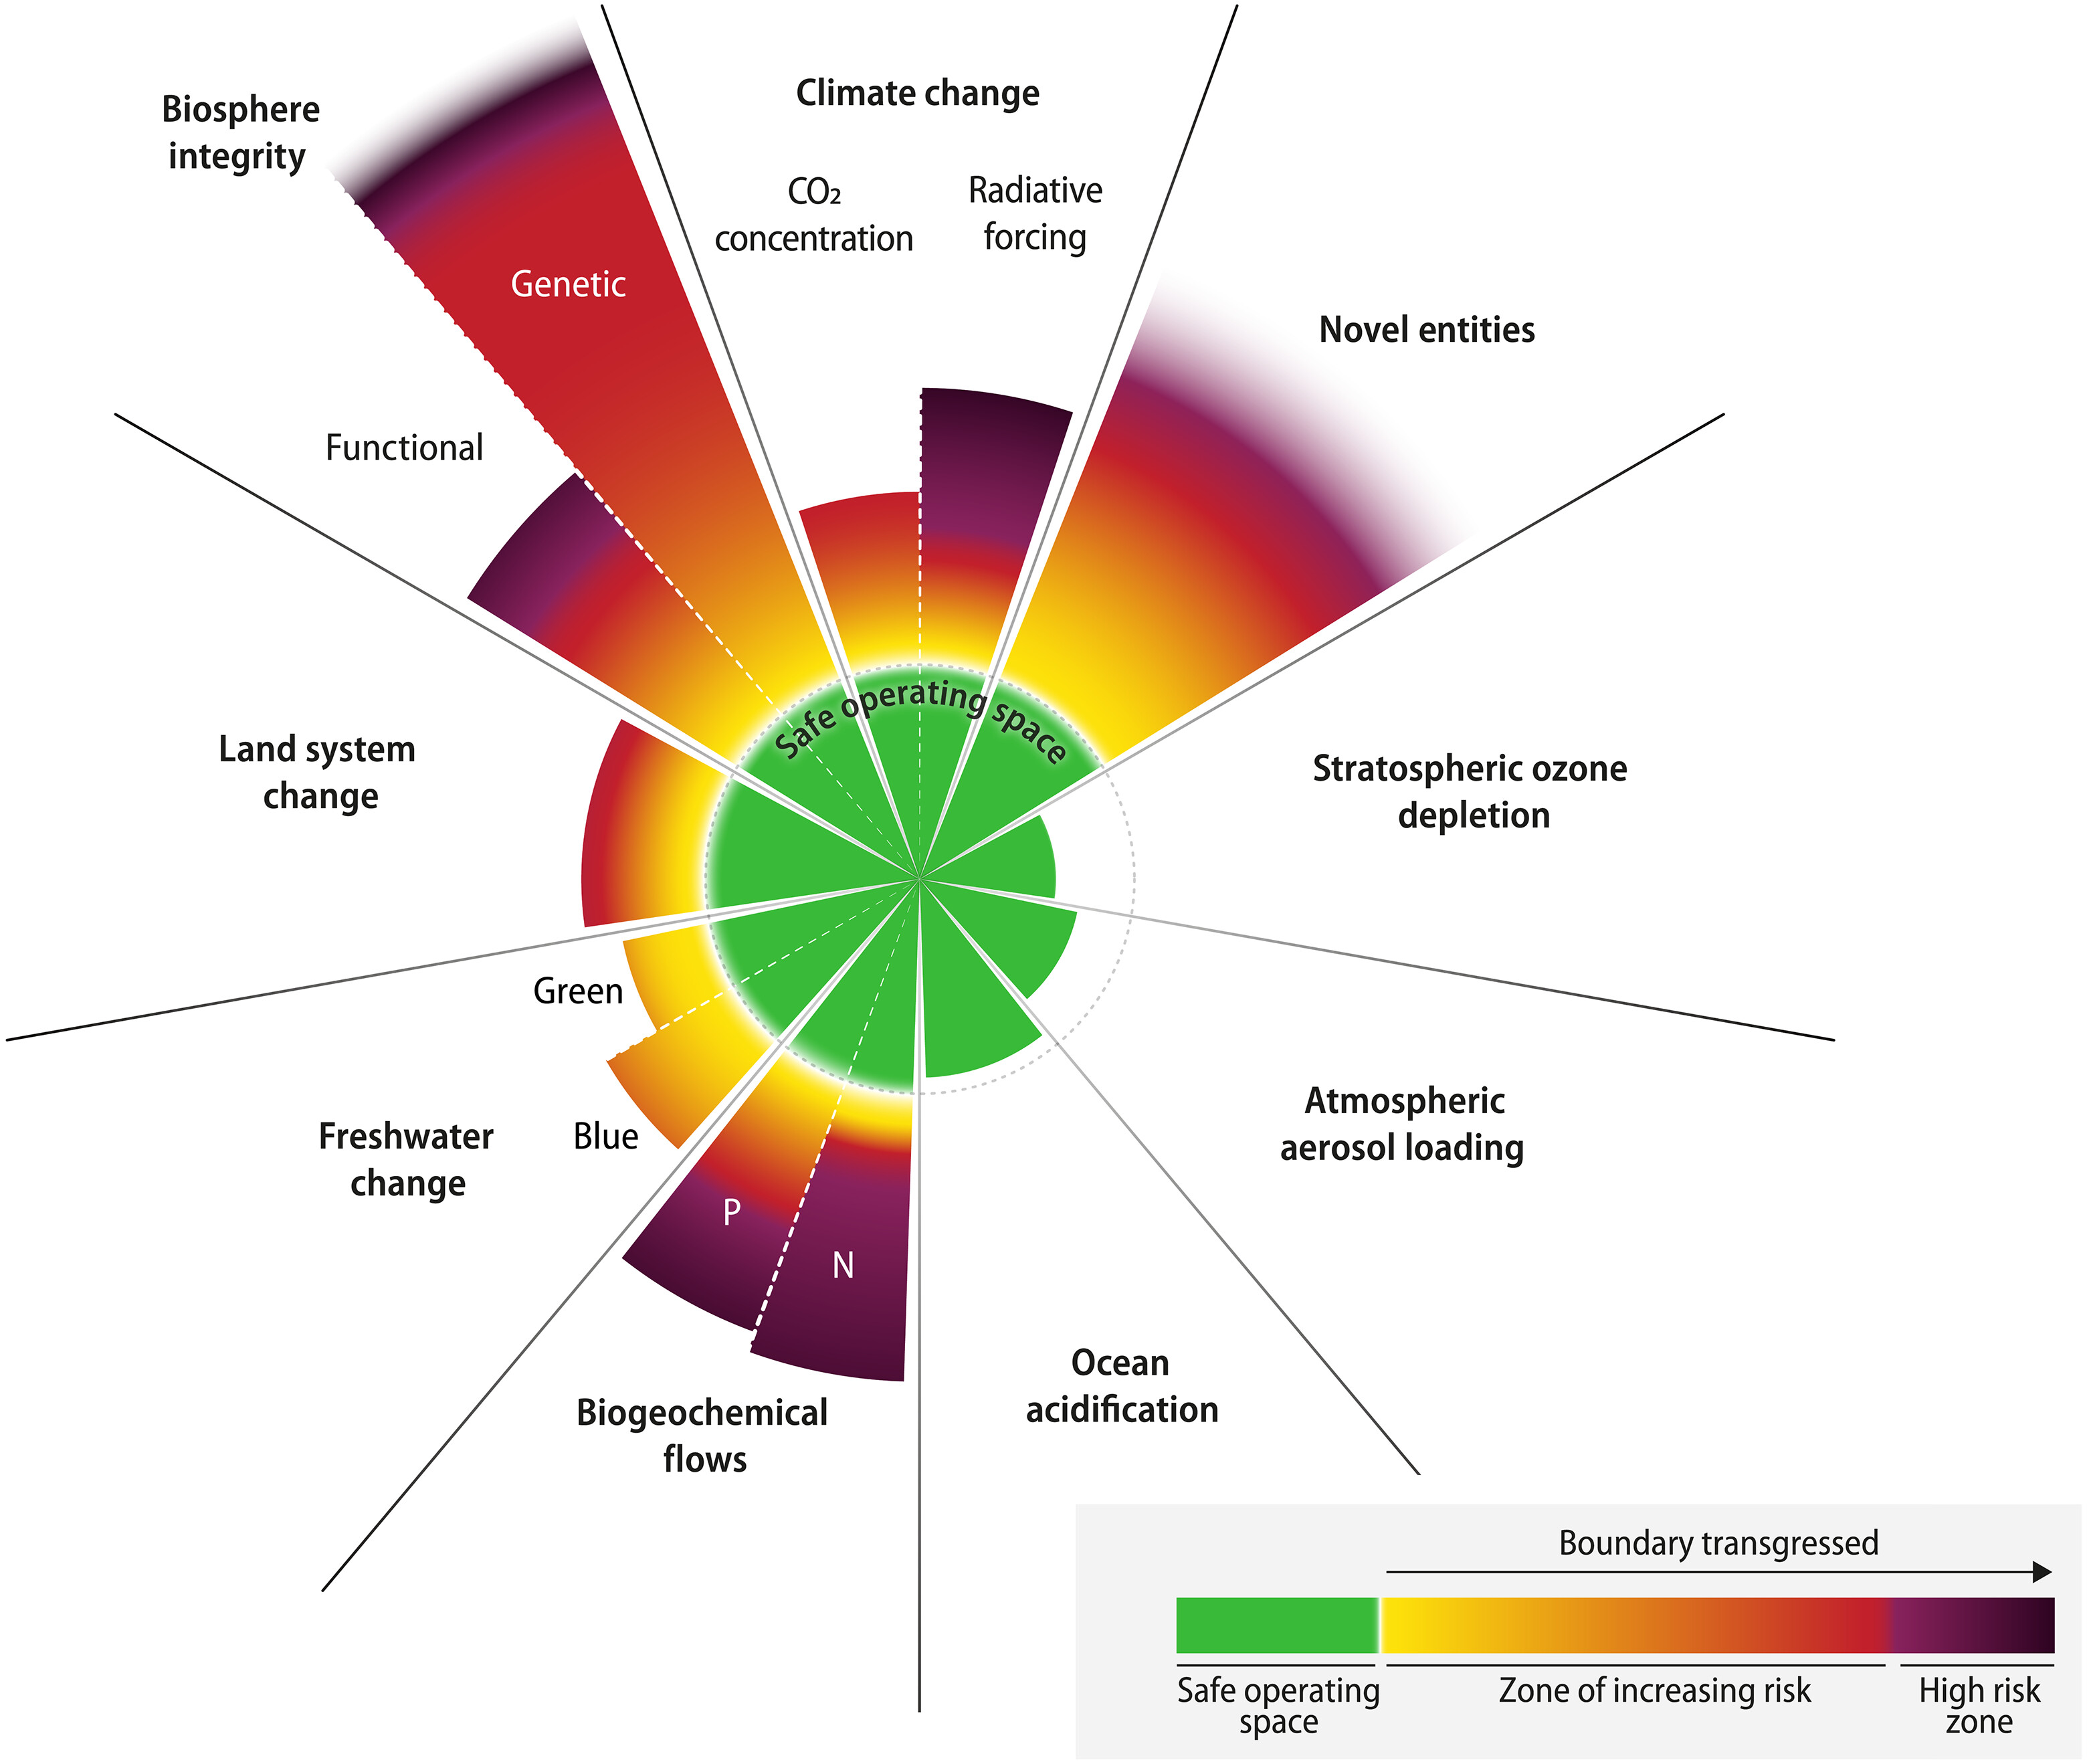
\includegraphics[width= .7\textwidth]{figures/intro/planetary_bounds.jpg}
	\caption{Current status of control variables for all nine planetary boundaries, from \cite{richardson_earth_2023}}
\end{figure}

Among these planetary limits, the integrity of the biosphere has gradually become of particular interest, along with its interaction with other limits, such as climate change, or novel entities (e.g. synthetic organic pollutants, radioactive materials, microplastic pollution...). Created in 2012, the Interdisciplinary Panel on Biodiversity and Ecosystem Services (IPBES) has been raising the alarm on the state of "Nature" globally. Its chair, Sir Robert Watson, put it clearly\footnote{See the \href{https://www.ipbes.net/news/Media-Release-Global-Assessment}{press release address of the 2019 report}}:
\begin{displayquote}
\textit{The overwhelming evidence of the \cite{ipbes_2022_6417333} Global Assessment from a wide range of different fields of knowledge, presents an ominous picture [...]. The health of ecosystems on which we and other species depend is deterioriating more rapidly than ever. We are eroding the foundations of our economies, livelihoods, food security, health and quality of life worldwide}
\end{displayquote}

"Nature" is a central concept in the IPBES framework \citep{ipbes_2022_6417333}:

\begin{displayquote}
\textit{Nature (also defined as living nature) [is] the nonhuman world, including coproduced features, with particular emphasis on living organisms, their diversity, their interactions among themselves, and with their abiotic environment. Within the framing of natural sciences, nature includes e.g. all dimensions of biodiversity, species, genotypes, populations, ecosystems, the biosphere, ecosystem functioning, communities, biomes, Earth life support's systems and their asosicated ecological, evolutionary, biogeochemical processes and biocultural diversity. Within the framework of economics, it includes categories such as biotic natural resources, natural capital, and natural assets. Within a wider context of social sciences and humanities and interdisciplinary environmental sciences, it is referred to with categories such as natural heritage, living environment, or the nonhuman. Within the context of other knowledge systems, it includes categories such as Mother Earth [...], Pachammama [...]}\\
\hspace*{\fill} \small{\cite{ipbes_2022_6417333}, p.14, see also \cite{DIAZ20151}}
\end{displayquote}

Nature, as defined in this approach, is a very large and complex object.
It is defined across ontological and epistemic differences (living and non-living e.g. matter), different types of interactions, at various scales (genotypes v. ecosystems), at different types of processes (biological v. ecological), and across different fields of inquiry (natural sciences v. social sciences). In this dissertation, I study more specifically "biodiversity", which focuses on the variability among living organisms. While it is itself an ambiguous concept, biodiversity tends to put the focus on living organisms, in relation to their material, biotic and abiotic environment (as opposed to the study of the non-living environment) and on its critical role among other components of the Earth system.

The \cite{ipbes_2022_6417333} report documents the drastic changes the biosphere is going through and considers these changes through an anthropocentric lense, i.e. mediating the aforementioned changes through the multiple and diverse contributions that Nature and biodiversity bring to people. It stresses how their disruption impacts human lives and highlights the role of anthropogenic (i.e. of human origin) drivers of the disruption of nature and biodiversity. 
 
This reports sets different objectives to scientific research. The first objective is to explain the feedback mechanisms : how do human livelihoods impact biodiversity? In response, how does biodiversity impact human livelihoods? This objective involves understanding the causes and measuring the direct and indirect anthropogenic drivers of change in nature and biodiversity on the one hand, and on the other hand understanding the channels and scales through which nature and biodiversity contribute to human livelihoods, as well as measuring these contributions. Hence, studying the demise of nature and the potential to remedy it calls for an integrated perspective, that joins natural sciences to social sciences, through frameworks such as social-ecological systems \citep{Ostrom2009} or environmental and ecological economics \citep{daly_ecological_2007}. 
\\
The second objective is to provide a framework to assess the desirability, the feasibility and means of implementation of collective pathways that would remedy the crisis nature is facing. In a way, it involves designing and implementing policy pathways towards sustainable futures, e.g. finding definite courses or methods of action selected from alternatives, at the individual, collective or governmental levels, to achieve future states of the world which remain in a safe operating space regarding planetary bounds \citep{rockstrom2009safe,steffen_2015_planetary}.

In this dissertation, I take on these two objectives using a framework stemming from economics and ecology. A first version of the research questions this thesis aims at solving is: 
\begin{enumerate}
\setlength{\itemsep}{0pt} % No space between items
\item What are the feedback relationships between biodiversity and antropogenic drivers of its decline? 
\item What underlying mechanisms must policy pathways tackle to remedy this demise?
\item  How can integrated economic and ecological approaches be used and refined to analyze inform and design policies? 
\end{enumerate}

In order to refine these questions, I first define the concept of biodiversity, through its natural and social sciences appraisals, and highlight ongoing trends in its demise.

\clearpage


\phantomsection
\addcontentsline{toc}{section}{Emergence and definition of biodiversity as an ecological concept}
\subsection*{Emergence and definition of biodiversity as an ecological concept}


Biodiversity emerged as a concept in the 1980s, along with the emergence of "conservation biology", a branch of biology concerned with the protection of "biological diversity" \citep{soule_what_1985}, as a response to an acceleration in the loss of species. The moral stance of conservation biologoy is that species should be protected for their own sake \citep{soule_conservation_1986}, they have intrinsic value. 
The concept of biodiversity is therefore embedded in an ethical judgement and a call for action. In the wake of the 1992 Rio United Conference on Environment and Development, the \href{https://www.cbd.int/}{Convention on Biological Diversity} emerged as an international treaty to safeguard biodiversity. In doing so, it provided an internationally agreed upon definition:

\begin{displayquote}
\textit{"Biological diversity" means the variability among living organisms from all sources including, inter alia, terrestrial, marine and other aquatic ecosystems and the ecological complexes of which they are part; this includes diversity within species, between species and of ecosystems.}\\
\hspace*{\fill} \small{\href{https://www.cbd.int/convention/articles/default.shtml?a=cbd-02}{Article 2 of the Convention on Biological Diversity}}
\end{displayquote}

This definition highlights a key differentiating feature from other parts of nature, i.e. the living nature of the objects of study. Compared to abiotic factors, biological diversity is characterized by intrinsic growth, reproduction and metabolism (at the individual and population levels), and evolution (at the genetic, and species level). Additionally, these rates of change through time are commensurable with human experience, and most processes (i.e. reproduction, population collapse or recovery, genetic evolution) can be observed within a human lifetime as opposed to the geological temporal scale. 

As highlighted by \cite{VanDyke2008} and \cite{mouysset_diversity_2023}, the definition of biodiversity is difficult, as it recovers ethical, conceptual and measurement dimensions. Biodiversity can be viewed as "an intrinsic, value-ladden quality of natural systems that should be preserved for its own sake" \citep{VanDyke2008, mouysset_diversity_2023}, but it also refers to measurable features.
% relevant to understanding genetic distribution, population levels, community structure (e.g assembly of interacting species in a given area), environmental processes, and ecosystem functions (i.e. the ecological processes performed by living organisms, such as carbon sequestration, nutrient recycling, water filtration etc). 
This definition implies different scales from a hierarchical perspective, at the genetic level, at the species, the community, and the ecosystem levels (defined as the interaction of communities and their abiotic environment). These levels imply different forms of measurement, including the distribution of genes, species abundance (i.e. the number of individuals in a population, at a given time and location), species richness (i.e. the number of different species, at a given time and location) within communities, among communities, and across larger scales (i.e. alpha, beta and gamma diversities.), as well as variations in the abiotic factors that form ecosystems, such as temperature, humidity, water quality, soil quality etc. 
It also comprises different types of diversity : structural diversity (for example, the layers of canopy in forests, the sex-ratio in animal populations), compositional diversity (the variety and abundance of species within a community), and functional diversity (variety of environmental processes performed by living organisms in a given area i.e. carbon sequestration, nutrient cycling or seed dispersal, see \cite{loreau_biodiversity_2002})

\begin{figure}
	\centering
	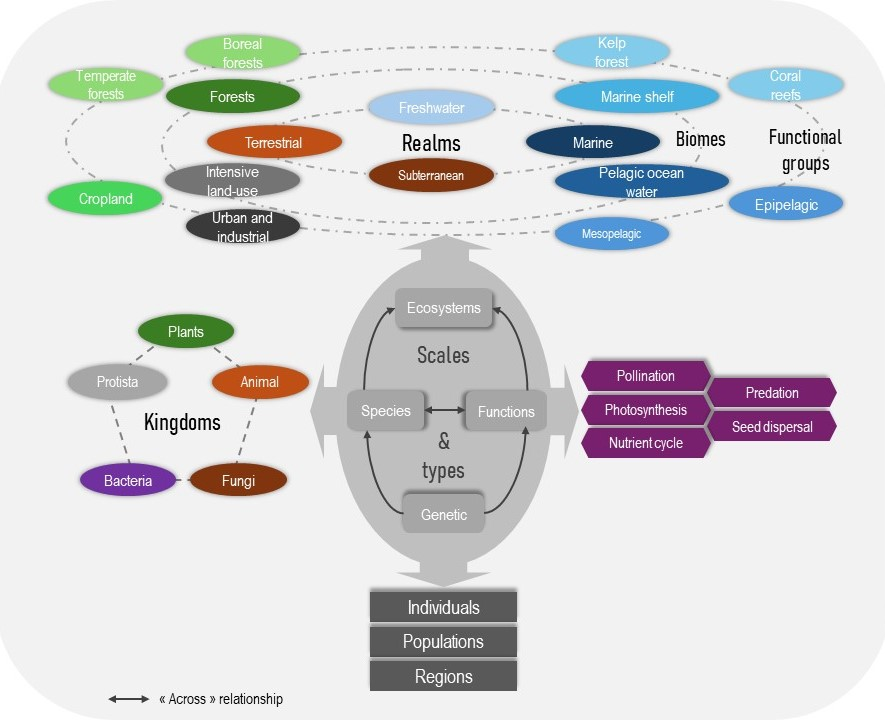
\includegraphics[width =.8\textwidth]{figures/intro/biodiv_illustration.jpg}
	\caption{Biodiversity : a multiform concept across scales and types}
	\label{fig:intro_biod}
\end{figure}

\cite{mouysset_diversity_2023} highlights the difficulty of articulating the definition with common levels in scientific analysis i.e. genetic, taxonomic, and ecosystem, as biodiversity level can fall in between: "populations may be considered from a genetic and taxonomic perspective, or communities that fall between the taxonomic and ecosystem levels". Additionally, as structural and compositional diversity can be seen as the source of functional diversity, the different classes of diversity may be difficult to work with given their colinearity. 

The multiple dimensions of biodiversity highlight several of its critical features. First, it is impossible to measure biodiversity with a single indicator. The study of biodiversity requires multiple indicators to integrally assess the evolution of biodiversity, across scales and types of diversity. The emergence of the concept responds to a desire to protect biodiversity for its own, but also humanity's sake. 

\clearpage

\phantomsection
\addcontentsline{toc}{section}{Nature's Contributions to People: rationales for biodiversity conservation}
\subsection*{Nature's Contributions to People: rationales for biodiversity conservation}


Originally descriptive, ecosystem functions were increasingly viewed from a human perspective starting in the 1970s \citep{hueting1969functions, schumacher1973small}, evolving into the concept of ecosystem services \citep{ehrlich1981extinction} to illustrate biodiversity loss consequences \citep{gomez_history_2010}. This marked a shift from intrinsic to anthropocentric (i.e. given by humans) value \citep{mouysset_diversity_2023}, recognizing biodiversity’s instrumental and relational values—serving human ends and fostering meaningful relationships. Gradually, biodiversity had to be protected for its role in sustaining human life.


%While originally descriptive, ecosystem functions have gradually been referred to from the human point of view (starting in the 1970s, see  \cite{hueting1969functions, schumacher1973small}) and how these functions served human societies, through the concept of \textit{ecosystem services} \citep{ehrlich1981extinction}, as a pedagogical tool to illustrate the consequences of biodiversity loss \citep{gomez_history_2010}.  In this respect, a value switch was operated from an intrinsic value towards an anthropocentric value (i.e. given by humans) standpoint \citep{mouysset_diversity_2023}. In more details, biodiversity features an instrumental value (i.e. serves to achieve a human end) and a relational value (i.e. the importance of desirable, meaningful, and often reciprocal relationships - beyond means to an end) : if biodiversity is to be preserved, it is because of the functions it performs that sustain and improve human life.

The concept gained traction in academic research, and as \cite{Costanza1997} quantified the value of natural capital and ecosystem services, at a staggering 33 trilion \$USD, amounting to approximately 30\% of the 2020 World GDP, the concept reached the policy arena. In 2005, the Millenium Ecosystem Assessment \citep{MEA2005} placed ecosystem services at the center of the policy agenda : it emphasized an anthropocentric value of ecosystem services, but established a dependence of human societies on ecosystem services, and further, on the functioning of ecosystem. In this respect, the Millenium Ecosystem Assessment \cite{MEA2005} was a landmark in safeguarding biodiversity through a \textit{strong sustainability} paradigm (see box 1), and triggered the operationalization of the concept into policy at a large scale (which I will develop later on). The ecosystem services framework was divided into 4 categories, relating to the specific type of services contributing to "human wellbeing" : supporting services (i.e. services allowing for other ecosystem services to be present, including nutrient cycling and primary production) and regulating services ("benefits obtained from the regulation of ecosystem processes" e.g pollination, waste decomposition etc); cultural services ("the nonmaterial benefits people obtain from ecosystems through spiritual enrichment, cognitive development") and provisioning services ("all the products obtained from ecosystems",\cite{MEA2005}, p.54)

\begin{figure}[h]
	\centering
	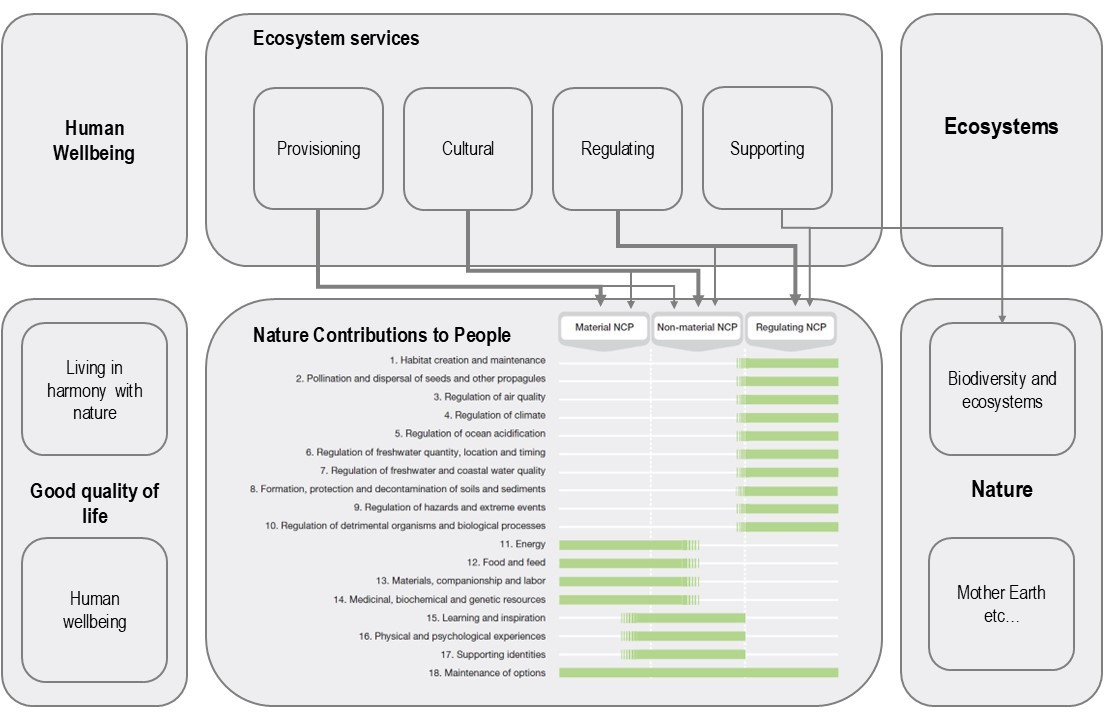
\includegraphics[width = \textwidth]{figures/intro/NCPs2.jpg}
	\caption{Description of the 18 Nature Contribution to People and the connection between the NCP framework \citep{ipbes_2022_6417333} and the Ecosystem Services Framework \citep{millennium2005ecosystems}}
	\subcaption*{Adapted from \cite{diaz_2018} and \cite{ipbes_2022_6417333}}
\end{figure}

Recently, the IPBES platform moved onto a new conceptual framework highlighting Nature Contributions to People (NCP) \citep{DIAZ20151}, defined as "all the contributions, positive and negative, of living nature [...] to people's quality of life \citep{diaz_2018}". This framework underpins 3 types of contributions to people: material contributions to people (flows from nature to people typically consumed to "operate a society or enterprise" (IPBES, p.16), non material contributions (eg. nature's effects on "subjective and psychological aspects underpinning peoples quality of life) and regulating contributions (i.e. "functional and structural aspects of organisms and ecosystems that modify the environmental conditions experienced by people and/or regulate the generation of material and non material contributions"). This framework highlights how Nature Contributions to People can be positive or negative, and depend on the spatial and temporal definition of the contribution, as a given entity can be at the same time the source of positive and negative contributions: for example, forests foster habitat, but also risk endangering people in the event of wildfires. Additionally, it provides a more encompassing view than ecosystem services, as it encompasses perspectives ranging from biodiversity as natural capital employed in an ecological production function (see \cite{polasky_integrating_2009} for a review), as well as perspectives where biodiversity has agency and is linked by reciprocal care obligations to humans \citep{descola}. 

A multifaceted correspondence between the different components and dimensions of biodiversity and its contributions to people underpin human livelihood. The global decline of biodiversity threatens NCPs.

\clearpage
\begin{tcolorbox}[breakable, 
colback=verylightgray, 
colframe=gray!75!black, 
title= {Box 1 - Weak v. Strong Sustainability},
%code={\singlespacing},
fontupper=\small]
\par % This \par ensures spacing before the text starts
\justifying % Start justified text

In 1987, the release of the Brundtland Report \citep{brundtland} provided a broad definition of sustainable development: 

\begin{displayquote}
\textit{In essence, sustainable development is a process of change in which the exploitation of
resources, the direction of investments, the orientation of technological development; and institutional change are all in harmony and enhance both current and future potential to meet human needs and aspirations}\\
\hspace*{\fill}\small{\cite{brundtland}, p.43}
\end{displayquote}

Implementing sustainable development remained an open question. In economics, a "weak sustainability perspective", pioneered by works of \cite{hartwick_intergenerational_1977} and \cite{solow_intergenerational_1986} on exhaustible resources, suggested that "maintaining a non-declining capital stock, which allegedly could be put into practice by investing in manufactured capital all the rents derived from the exploitation of non-renewable natural resources" \citep{gomez_history_2010} was sufficient to maintain consumtpion through time. In this approach, natural capital could be integrally substituted by human made capital. On the other hand, the "strong sustainability" approach advocates advocates for a complementarity, rather than substitutability, of natural resources \citep{costanza_daly}, acknowledging the dependence of humans on ecosystems.
\end{tcolorbox}

\phantomsection
\addcontentsline{toc}{section}{Decline in biodiversity : trends and drivers}
\subsection*{Decline in biodiversity : trends and drivers}

Biodiversity metrics are declinning across all the scales of analysis. The structural conditions of ecosystems, the compositions of ecological communities and populations of species have experienced dramatic changes.\\
The share of unchanged, protected wildlife habitat has plumetted on both land and sea \citep{watson_2016_catastrophic, jones_2018_location} to 23\% and 12\% of space, respectively. At the community level, the share of originally present biodiversity falls bellow 90\% across all biomes, \citep{Hill311787} and local communities are becoming more and more similar \citep{mckinney_1999_biotic}, driven by the increased extent of animal and plant non-alien invasive species, rising by 13\% per decade \citep{seebens_no_2017}. At the species level, to date, global species richness is threatened by a mass extinction, as the global rate of species extinction is at least ten times higher than the average rate over the past 10 million years and is accelerating \citep{barnosky_has_2011, ceballos_accelerated_2015}. On average, 25\% of species are currently threatened with global extinction across a wide range of plant and animal species, on land and at sea \citep{IUCN_redlist_2024}. Using habitat based methods\footnote{ The IUCN Redlist uses detailed accounts for species, in a bottom-up approach, to analyze the extinction risk of species. A top-down approach, relying on the evolution of available habitat and the species-area relationship, uses changes in land use to forecast the extinction of species in a more aggregate manner \citep{Diamond1972BiogeographicKE}}, \cite{Hoskins309377} find that hundreds of thousands of plant and animal species are threatened, and will repay the \textit{extinction debt} caused by anthropogenic changes to their habitats : only 92.1\% of terrestrial vertebrate species, 91.6\% of terrestiral invertebrates and 90.7\% of terrestrial plants have enough habitat to persist. These results suggest that around half a million terrestrial animal and plant species - including over 3000 vertebrates and over 40,000 plants - \textit{dead species walking}, doomed to become extinct, unless their habitats improve in time to prevent it \citep{ipbes_2022_6417333}.

%\begin{figure}[h]
%    \centering
%    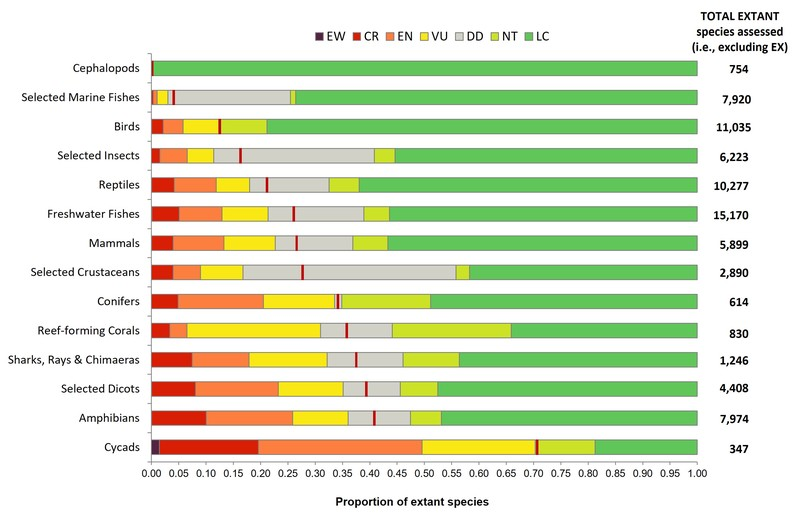
\includegraphics[width=0.8\linewidth]{figures/intro/IUCN_redlist}
%    \caption{The proportion of extant (i.e., excluding Extinct) species in \citet{IUCN_redlist_2024}}
%    \subcaption*{Assessed in each category for the more comprehensively assessed (i.e., at least 80\% of the group has been assessed) groups containing $\geq$ 150 species. Species are grouped into classes. The numbers to the right of each bar represent the total number of extant species assessed for each group. \textbf{EW} - Extinct in the Wild, \textbf{CR} - Critically Endangered,\textbf{ EN} - Endangered, \textbf{VU} - Vulnerable, \textbf{NT} - Near Threatened, \textbf{DD} - Data Deficient, \textbf{LC} - Least Concern.}
%    \label{fig:intro_iucn}
%\end{figure}

Drivers of biodiversity decline are of anthropogenic origin. They can be classified between \textit{direct} drivers, i.e. that directly flow form human actions, such as land use change, anthropogenic climate change, overexploitation, and \textit{indirect} drivers, that can be viewed as the root cause for direct drivers, such as  , changes in the value systems that underpin nature uses (\cite{ipbes_2022_6417333} p.55), demography (urbanization and migration), technology, economy (sectoral transitions, trade expansion) and governance (including risht systems for access to resources).

%The Essential Biodiversity Variables framework \citep{pereira_essential_2013} aggregates fine gridded spatial data into 
A synthesis of natural sciences performed by \cite{ipbes_2022_6417333} outlines the roles of principal drivers at the global scale and across realms (see figure \ref{fig:intro_impacts}).
It shows that land and sea use, reefering to the loss, fragmentation\footnote{Undoubtedly, habitat loss is the main driver of terrestrial biodiversity decline. The effects of fragmentation on biodiversity are highly debated. From a theoretical perspective, models have been developed to study the evolution of populations and communities through space and time, i.e. metapopulation and metacommunity models. Theoretical insights highlight that habitat fragmentation increase the extinction risk, and lower colonization probability, resulting in lower survival and diversity \citep{adler_persistence_1994,hill_habitat_1999, thompson_loss_2017}. At the community scale, increases in diversity among communities (i.e. beta diversity) can emerge from different species resource requirements and the larger spatial extent, hence encompassing more environmental heterogeneity, that results from fragmentation \citep{lasky_reserve_2013, chisholm_species_2018}. However, these effects dampen as habitat loss decreases.  
At the empirical level, the effect of fragmentation is highly debated. According to \cite{fahrig_ecological_2017}, there is no empirical evidence that a group of small habitat patches generally has lower ecological value than large patches of the same total area. Evidence is however found to show that fragmentation does not reduce habitat connectivity, as functional connectivity is improved (i.e. species are in contact with more different resource patches, thus improving the overall functionning of ecosystems). The debate between \cite{fletcher_is_2018} and \cite{fahrig_habitat_2019} surrounds critics based on the ability of statistical models to encompass the effect of fragmentation when habitat loss is present \citep{ruffell_accounting_2016}. Moreover, it reflects the difficulty of landscape ecology, as different mechanisms across scales i.e. patch, landscape and study region, and measures, such as patch size, patch isolation (i.e. distance across patches) and distance to patch edge (i.e. distance to edge within the patch) interact with possible non-linear interactions.}
%
and degradation of wildlife habitat are responsible for 30\% of the impacts on biodiversity. The direct exploitation of wildlife, wild plants and trees represents 23\% of impacts. Climate change, through shifts in biogeographic conditions and changes in habitat, impacts on species traits and genetic evolution represents 14\%, and pollution represents 14\% of impacts. Finally invasive alien species represent 11\%. These drivers have differenciated impacts across ecosystems and biomes \citep{ipbes_2022_6417333}. 

\begin{figure}[h]
	\centering
	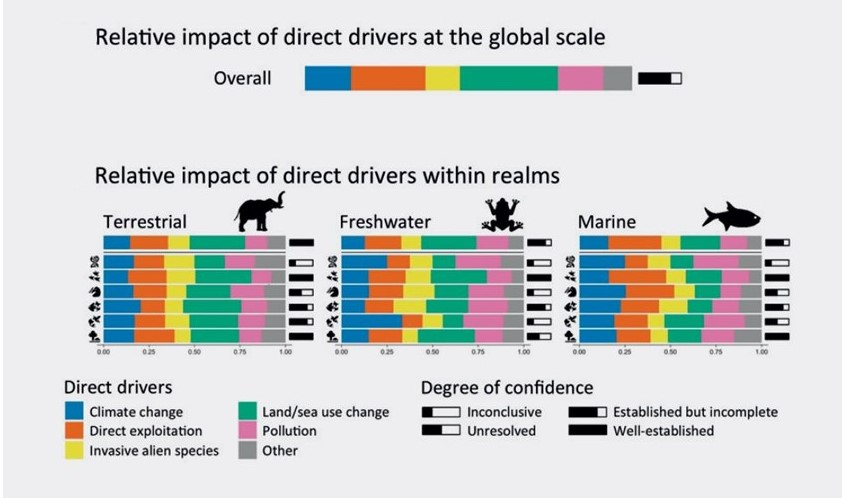
\includegraphics[width = .95 \textwidth]{figures/intro/intro_impactsfin.jpg}
	\caption{Aggregate and realms specific impacts of anthropogenic direct drivers of biodiversity decline adapted from \cite{ipbes_2022_6417333}}
	\label{fig:intro_impacts}
\end{figure}

On land, land use change is the most important driver (30.5\%), driven by deforestation and agriculture, and direct exploitation follows next (21\%). Tropical and subtropical dry and humid forest host the greatest biological diversity. For example, they host the 10 hotspots with the greatest total number of vertebrates \citep{mittermeier_global_2011}. In such forests, habitat loss and degradation are the main drivers of reductions in species abundance and richness \citep{newbold_global_2014}. Legal and illegal selective logging destroy habitat \citep{hoare2022establishing,  bousfield_2023_large} and are combined with hunting and poaching of wildlife \citep{gallego_2020_combined}, generating between 60 and 180 billions  \$ USD of revenue \citep{gfi_2017}\footnote{Illegal wildlife trade represents between 5 and 23 billion \$USD, while illegal logging represents 52 to 157 billion \$USD}. 

For marine species, overexploitation is the main driver (29\%) \citep{ipbes_2022_6417333}. With 90 million tons of capture  (and 141 billion \$ USD)  in 2020 \citep{fao_2022_state}, fisheries stock within biologically sustainable levels have decreased to 64.6\% in 2019, from 90\% in 1974\footnote{ In this calculation, all fishery stocks are equally counted, irrespective of their abundance or catch}, driven by overfishing in the Southeast Pacific and the Mediterranean and Black seas. Nonetheless, illegal, unreported and unregulated (IUU) fishing is a threat to fisheries. Estimates from 15 years ago \citep{agnew_estimating_2009} estimated it represented between 11 and 26 million tonnes of fis with a value of 10 to 23 billion \$ USD. 
 
Additionally, anthropogenic climate change drives ecosystem disruptions on land \citep{burrell_anthropogenic_2020, conradi_reassessment_2024} and at sea \citep{gomes_marine_2024}, through changes in various channels including ecological suitability and foodweb disturbances. On land, for example, mediterranean forests, woodlands and scrubs, covering 4 million km$^2$, are areas of exceptionally high diversity too \citep{Mooney2001, blondel_2010}, threatened with urban expansion and increased wildfire risk. Wildfire frequency and severity are expected to increase with global warming \citep{Dupuy2019ClimateCI}, causing important direct and indirect costs to society including destruction of infrastructure and perturbations to economic activity \citep{wang_economic_2021}, smoke related health conditions \citep{burke_wildfire_2023, heft-neal_behavior_2023}, disrupting structural features of ecosystems \citep{Ayars2023} and threatening biological diversity \citep{Wintle2020}.

\phantomsection
\addcontentsline{toc}{section}{Economic challenges of anthropogenic drivers of biodiversity decline}
\subsection*{Economic challenges of anthropogenic drivers of biodiversity decline}

Habitat loss and overexploitation present both common and differentiated challenges. A common identifiable cause is the large opportunity cost of preserving a species habitat, or existence, in the presence of other economic alternatives for land and time, as well as financial constraints. Additionally, habitat loss and overexploitation share a temporal dynamic aspect, where immediate actions have durable consequences, possibly irreversible.

Habitat loss and fragmentation in terrestrial ecosystems present specific challenges. Forests, for example, serve multiple uses (or NCPs) to various agents: loggers profit from timber, settlers clear land for agriculture, hikers seek pristine landscapes, and conservationists aim to restore natural cycles. Forests also hold spiritual and cultural value, creating conflicts among these uses. For instance, deforestation and urbanization destroys both habitat and sacred land, but create measured economic value \citep{giglio_economics_2024} while wildfire prevention can damage wildlife habitat \citep{bradshaw2018}. Species can also have mixed impacts; deer, for example, are valued at low densities but cause damage at higher densities \citep{putman_identifying_2011}. 
%Climate change worsens habitat loss by altering habitat distribution and increasing threats like wildfires \citep{Dupuy2019ClimateCI,wasserman_climate_2023}\\
A second key feature to halt habitat fragmentation is considering the integral set of interdependencies, ecological spillovers and economic externalities that underlie the spatial dimension. The configuration of space, and species movement is at least partly the result of an economic decision. Maintaining habitat connectivity involves identifying patches and paths to be conserved or restored that contribute most to it, in the form of corridors, ecoducts or stepping stones \citep{Turner2005, Turner2011}. The value of patches and paths for connectivity is intrinsically linked to their surrounding : at the same geographic location, a patch has differential value for biodiversity habitat if it is connected to others, or if it is isolated (see box 2). When paths are beyond human control, patches have different importance based on their location, and when the location of patches is fixed, the extent of paths and their location is paramount. Third, as multiple actions and uses structure connected elements of ecosystems (i.e. different tracts of land, or different biodiversity scales), they trigger spatial spillovers i.e. consequences that go beyond their \textit{in situ} effects. When these spillovers are not taken into account by the agents that generate them, they can be called "dynamic spatial externalities" \citep{sanchirico_bioeconomics_1999, costello_optimal_2008, costello_private_2017}. As halting habitat loss and fragmentation involves conserving tracts of land, neighboring parties may very well benefit (or suffer) from more wildlife and ecosystem (dis-)services on their property, through time. As agents respond to each other's action profiles, they behave strategically, both in space and time. These externalities can trigger specific problems of "race to the bottom" \citep{costello_private_2017} : when neighboring parties of a decision maker that undertakes conservation, or risk reduction, fail fail to reciprocate as they benefit from spillovers, a vicious circle of least action is triggered. Conversely, when ecological spillovers are positive, this may lead everybody to use a resource at unsustainable levels, even in the presence of well defined rights, absent other mechanisms \citep{janmaat_sharing_2005,kaffine_unitization_2010}. 
 Hence, habitat fragmentation and overexploitation are interrelated through spatial connectivity. Fourth, improving habitat loss and fragmentation involves coordinating numerous actors towards increasing the area and connectivity of habitat, while taking into account the associated costs and benefits, and different interests.
 In some cases, the financial constraints, the magnitude of costs associated with increased habitat connectivity and the difficulty of coordination warrant a public policy where a central planner undertakes the action \citep{Mouysset2012}. On the other hand, mechanisms to decentralize efficient spatial planning exist and can be efficient under limited costs of cooperation \citep{costello_private_2017, bareille_agglomeration_2023}. 
 
	Halting overexploitation requires understanding and addressing its motives. Overexploitation (or under control, for pests), results from an imbalance between the appropriation and incumbance of Nature's contributions to people (both positive and negative) and the socially desirable level and allocation of these contributions, as well as the uncoordinated, strategic behavior of agents. 	
	The common nature of most natural resources \citep{Gordon1954, smith_models_1969} has long been identified as one of key reason for their demise: numerous events have shown a "race to the bottom", where the absence of secure property rights hastened the overharvest and decline of populations. It has long been the center of attention, and mechanisms relying on property rights assignment have been studied extensively \citep{libecap_tragedy_2009, costello_partial_2015, isaksen_tragedy_2019}.\\
	
\begin{tcolorbox}[breakable, 
colback =verylightgray, 
colframe=gray!75!black,
title={Box 2 - Habitat Loss, Fragmentation and Connectivity},
%code={\singlespacing},
fontupper=\small]


\par % This \par ensures spacing before the text starts
\justifying % Start justified text

Habitat loss refers to the loss of areas featuring suitable environmental conditions for species survival and development. At a constant habitat area, fragmentation refers to increases in the number of patches and decrease in the mean size area of each patches, as in figure \ref{fig:connectivity_intro}. \\
Landscape connectivity is defined in relation to fragmentation. It measures "the degree to which the landscape facilitates or impedes movement among resource patches" \citep{taylor_connectivity_1993}. 
It recovers a \textit{structural} dimension, which describes the physical arrangements across patch and a \textit{functional} dimension, which emphasizes the ability and realization of movements of individuals through the landscape.

 Aggregate connectivity measures take into account the role of differentiated patches and paths. In panel D of figure \ref{fig:connectivity_intro}, the circled patches play an instrumental role in maintaining connectivity. Habitat patch 1 and 2 have the same number of connected patches. However, patch 1 is maintains the connection between the east and west habitat patches in the landscape, and is connected to highly connected patches. Removing habitat patches 1 and 2 would have larger consequences on habitat than removing other identical size patches. Similarly, removing the dotted path (bottom left of panel D) would isolate patch 3, while removing the dashed path would not leave patch 4 isolated. Hence, paths and patches have different impacts on connectivity, depending on the surrounding patches and paths.
\\% Adds some space before the image
\begin{center}
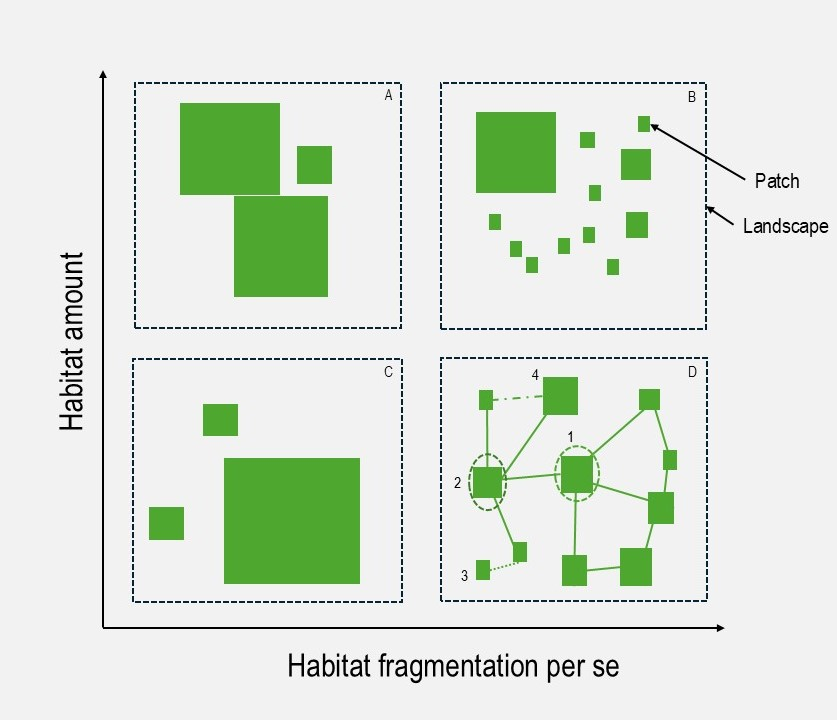
\includegraphics[width = .8\textwidth]{figures/intro/fragmentation.jpg}
\captionof{figure}{Illustration of the effects of habitat loss and fragmentation, adapted from \cite{fahrig_habitat_2019}, and of connectivity}
\label{fig:connectivity_intro}
\end{center}
\end{tcolorbox}
\clearpage
	
	 However, while property rights may be assigned, they can be notoriously hard to enforce in areas where regal functions are challenged: \textit{de facto} rights are assigned and enforced. In this case, the common nature of the resource may not be the main concern: local market concentration forces may outweigh overexploitation forces, even in the presence of some of form of open access \citep{damania_economics_2007}. 
Around the world, wildlife poaching and trade typically originates from organised crime groups, and is associated with different criminal activities \citep{mozer_introduction_2023}.  Concentrated markets tend to emerge and characterize wildlife markets, as competition is hindered by violent organised crime groups. In this case, resource management is strategic and responds to market characteristics (demand structure, intermediary input price) and ecological characteristics (distribution of species, biological growth rate, carrying capacity\footnote{The notion of \textit{carrying capacity} has been used since the mid-XXth century by population ecologists (for a history of the notion, see \cite{sayre_carrying_2008}) to describe the maximum population size of a species a given ecosystem can sustain in the long run.} of the ecosystem)\\
	At one extreme, locally monopolistic markets structure for wildlife products may emerge, especially in the case of endemic species (i.e. native and restricted to an area).
They may be the conservationists' bestfriend \citep{solow_resources_1974, hannesson_note_1983}, depending on specific, context dependent market and species characteristics, as a monopolist has an interest in restricting supply to increase prices, if consumers do not react too much (i.e. under limited demand elasticity). A vast range of  market structures \citep{damania_economics_2007, hannesson_effects_1985} sticking to real world situations have been studied. However, the full range of interactions between a species endemism, local market power, cost of effort and access to final consumer markets require more analysis to clarify the impact of market structure.\\
	Other drivers of overexploitation can be found in the large expected benefits (relative to other local economic activity) some natural resources can bear, most of the time because of their rarity (i.e. absence of economically viable substitute), whether today or in the future \citep{Kremer2000}. While the effects of substituting man-made products to disrupted ecosystem services are starting to get empirically studied \citep{frank_economic_2024} and show how dreadful costs can be, the effect of introducing substitutes to illegally poached wildlife products can be an example of strong substitutability between natural and man-made assets \citep{chen_economics_2017}. As broader forces affect overexploitation, including poverty, it is clear that adressing overexploitation implies generalizing conclusion from the interplay of a single species with the institutional setting, how a  species' future interacts with the availability of substitutes, and how the distribution of revenues from sustainable harvests may foster a reasoned use of the resource. 
	
	A wide range of policies have been implemented at different organisational levels, to jointly or separately halt the identifed drivers of biodiversity decline on land and at sea, with varying degrees of success. 

\phantomsection
\addcontentsline{toc}{section}{Biodiversity policies : from global to local}
\subsection*{Biodiversity policies : from global to local}
\par
Successive international policy frameworks have sought to halt biodiversity loss by addressing its drivers comprehensively. In 2022, the 15th conference of the UN Convention on Biological Diversity launched the \href{https://www.cbd.int/doc/c/e6d3/cd1d/daf663719a03902a9b116c34/cop-15-l-25-en.pdf}{Keunming Montreal Global Biodiversity Framework (GBF)}, replacing the Strategic Plan for Biodiversity 2011-2020 and the Aichi Targets after the failure to meet its objectives\footnote{Among the 20 Aichi Targets, none were globally met in 2020, and only 6 were partially met including the identification and eradication of invasive species on islands, the setting of 17\% of terrestrial and inland water areas and 10\% of coastal and marine areas as conservation areas, the implementation of policy instruments and effective national biodiversity strategy and planning, and the increase in financing biodiversity protection. Reasons invoked for the failure were the lack of clear indicators to assess targets, and no obligation to report on progress towards achieving the targets  \citep{maron_setting_2021}}. The GBF sets four global goals for 2050, with 23 measurable targets to halt biodiversity loss by 2030. These goals include maintaining ecosystem integrity and connectivity and preventing human-induced extinctions (Goal A), sustainably using biodiversity (Goal B), sharing conservation benefits and burdens equitably (Goals C and D)\footnote{See \href{https://www.cbd.int/doc/c/e6d3/cd1d/daf663719a03902a9b116c34/cop-15-l-25-en.pdf}{Section G. Kunming-Montreal Global Goals for 2050}}. \href{https://www.cbd.int/gbf/targets/5}{Targets} include restoring 30\% of degraded ecosystems, conserving 30\% of land and sea areas, and ensuring the sustainable use and management of wild species.



%\begin{tcolorbox}[breakable, 
%colback=verylightgray, 
%colframe=gray!75!black,
%title={Box 3 - The Convention on Biological Diversity and the Aichi Targets},
%code={\singlespacing},
%fontupper=\small]
%\label{box:policy_frameworks_for_biodiv}
%\par % This \par ensures spacing before the text starts
%\justifying % Start justified text

%In 2010, the Convention on Biological Diversity set its "Strategic Plan for Biodiversity 2011-2020", structured around the 20 Aichi Biodiversity Targets, spanning over 5 goals :

%\begin{itemize}
%\item Goal A : Address the underlying causes of biodiversity loss by mainstreaming biodiversity across government and society
%\item Goal B : Reduce the direct pressures on biodiversity and promote sustainable use
%\item Goal C : To improve the status of biodiversity by safeguarding ecosystems, species and genetic diversity
%\item Goal D : Enhance the benefits to all from biodiversity and ecosystem services
%\item Goal E : Enhance implementation through participatory planning, knowledge management and capacity building
%\end{itemize}

%In 2020, the Global Biodiversity Outlook 5 \citep{global_biodiversity_outlook} showed that none of the Aichi %Target were globally met, and only 6 targets were partially achieved, including the identification and eradication of invasive species on islands, the setting of 17\% of terrestrial and inland water areas and 10\% of coastal and marine areas as conservation areas, the implementation of policy instruments and effective national biodiversity strategy and planning, and the increase in financing biodiversity protection. 

%While several elements showed progress, the failure of the 2011-2020 Strategic Plan was patent. Measurable indicators to assess progress towards targets were missing. This was tackled with the new Global Biodiversity Framework that took over in 2020, although with severe limitations. According to critics \citep{maron_setting_2021}, the current framework also lacks ecological scale-specific indicators (for genes, species, ecosystems) and do not provide specific net outcome statements (such as the 1.5C degree target of the Paris Agreements) across areas, nor a clear implementation timeline. 

%Additionally, the 2011-2020 Strategic Plan failed as countries did not have to report on their progress, only declare their targets. The 2020 Global Biodiversity Framework has implemented follow-up measures : although it is not a legally binding frameworks, countries who have signed commit to demonstrating progress towards the targets and update their National Biodiversity Strategy and Action Plans (see section B.5 and section J of the \href{https://www.cbd.int/doc/decisions/cop-15/cop-15-dec-04-en.pdf}{GBF})
%\end{tcolorbox}
Other international treaties, such as the \href{https://cites.org/fra}{Convention on International Trade in Endangered Species (CITES)} established in 1973, regulate trade in endangered species to prevent illegal wildlife trade\footnote{CITES features 183 member parties (countries), it lists species across "appendices", with varying degree of protection of the species and restrictions limiting the trade in endangered species.\\
Appendix 1 : the most endangered species, threatened with extinction and prohibited international trade, except when the purpose of exports is not commercial\\
Appendix 2 : species that are not necessarily now threatened with extinction but that may become so unless trade is closely controlled\\
Apppendix 3 : species included at the request of a Party that already regulates trade in the species and that needs the cooperation of other countries to prevent unsustainable or illegal exploitation} and promote species survival. Despite its scope, CITES’ effectiveness is debated. Local enforcement \citep{HEID2023102784} and demand reduction campaigns \citep{macfarlane_reducing_2022, moorhouse_demand_2024} are critical, but trade bans can sometimes increase prices and poaching incentives \citep{hsiang_does_2016}. In some cases, conservation farming has succeeded by “flooding the market” \citep{gentry_looking_2019, phelps_framework_2014, tensen_under_2016}. Supply-side interventions have occasionally succeeded at reducing poaching and recovering wild populations – i.e. vicuña and spotted cat \citep{iucn_world_2000, sahley_biological_2007} – but they have also failed – i.e. green python, African elephant \citep{lyons_wildlife_2011, hsiang_does_2016}. Uncertainty around conservation outcomes from market-based approaches has led to continued reliance on trade bans and controls that are often ineffective at reducing poaching.

National and supranational policies have also been key. In the U.S., policies like  \href{https://www.fs.usda.gov/Internet/FSE_DOCUMENTS/fseprd645666.pdf}{Wilderness Act of 1964} created protected areas to preserve habitats. In the wake of the environmentalist movement of the 1960s and 1970s, landmark regulations aimed at protecting natural habitats, such as the \href{https://www.epa.gov/laws-regulations/summary-clean-water-act}{Clean Water Act of 1972} (ensuring sewage to limit the disruption of wildlife habitat), and specifically targeted towards species conservation with the \href{https://www.fws.gov/sites/default/files/documents/endangered-species-act-accessible.pdf}{Endangered Species Act of 1973}. Results of the Endangered Species Act are debated. While the impacts seem to be overall positive on species recovery, budget dedicated to listings are slim, and the associated costs are substantial and concentrated on private landowners while benefits are more broadly distributed \citep{brown_economics_1998, langpap_economics_2018}.
%
Localized initiatives, such as the \href{https://y2y.net/}{Yellowstone Yukon Conservation Initiative} (1993), connect ecological areas across the U.S. and Canada, using private conservation schemes and local policy making. 
%
In Europe, the Natura 2000 network\footnote{A system of protected areas, established in application of the European Union Birds Directive (1976) and Habitats Directive (1992), and formally in place starting the mid 2000s} has created the largest conservation area globally, covering 18\% of land and 9\% of marine regions in the EU, across 28,000 sites. In broad strokes, it delineates conservation areas of ecological interest where development and human activities are restricted. Its ambition stemmed from taking into account the scale of biodiversity processes rather than administrative boundaries to develop an interconnected network of conservation areas. The ecological and economic performances of such a network are substantial, as they generate spatial spillovers both in terms of economic and ecological performance \citep{cocco_relaxing_2023}.

Acknowledging that biodiversity habitat can be seen as a continuum between unsuitable and suitable conditions, mechanisms such as Payments for Ecosystem Services (PES) are leveraged to incentivize conservation on agricultural land. Taking into account the ecological spillovers of decreased spillovers, payments for ecosystem services with agglomeration bonuses, such that neighbors gain an additional marginal benefit when a new local participant implements conservation measures, can be efficient \citep{parkhurst2002agglomeration, bareille_agglomeration_2023}. Overall, the spatial consequences of decentralized policies has yet to be fully integrated in policy making.

Finally, some policies aim at mitigating the threats posed by climate change on ecosystems and species, by changing landscape connectivity. In mediterranean forests, where biodiversity is exceptionally high but wildfires are an ever growing threat \citep{Dupuy2019ClimateCI, wasserman_climate_2023}, fuel treatment operations\footnote{Mechanical thinning, prescribed burns, and sometimes, logging, have been leveraged to decrease the fuel load in risky areas and theoretically decrease the probability and severity of burns upon wildfire occurence. In numerous regions, such as conifer forests in California \citep{Vaillant2009, Kalies2016, low_shaded_2023}, eucalypt forests in South Western Australia \citep{burrows2013, boer_long-term_2009, Florec2020}, southern Europe \citep{Fernandes2013}, evidence shows that fuel treatments, can mitigate wildfire intensity and spread. Land management agencies have historically implemented these policies in Australia \citep{burrows2013}, Europe, and the United States (and are projected to ramp up, for example under the Infrastructure Investment and Jobs Act of 2021 in the US)} limit the occurence and severity of wildfires. Public policy is leveraged in the face of increasing risk, limited insurability and threats to biodiversity. For example, with limited insurability of homes in the wildland urban interface in California\footnote{For example, \href{https://www.washingtonpost.com/climate-environment/2024/08/29/california-insurance-wildfires-allstate/}{200,000 homeowners will see an increase in their insurance premium} by an average of 34.1\% from Allstate insurance in November 2024. In 2023, the FAIR plan, designed to be the insurer of last resort in California (state mandated but privately funded) saw a \href{https://www.cfpnet.com/key-statistics-data/}{38.3\% increase in its total exposure.}}, as well as the potential economy-wide human and non-human damages from wildfires \citep{wang_economic_2021, heft-neal_behavior_2023, Ayars2023} state-mandated and operated fuel treatment policies are of the essence. However, with increased budgets and improved spatial planning, these policies could achieve better performances in reducing risk while protecting biodiversity.\\
Decentralized policy mechanisms exist, such as mandates to create a defensible buffer around individual properties : in California, a 100-foot defensible around houses is mandated in State Responsibility Areas,and can translate in reduced insurance premia;  in France, in dedicated regions, the "obligation de débroussaillement" mandates fuel control operations in a 50m radius to "decrease the intensity of wildfires and limit their spread"
\footnote{Translated by the author - \href{https://www.legifrance.gouv.fr/codes/article_lc/LEGIARTI000047809197}{Article L131-10} of the Code Forestier} with fines reaching $5,000$ euros for failing to comply.


I focus on the analysis of the interplay between biodiversity and human actions, through the NCPs it provides and the anthropogenic drivers of its decline. As existing policies have had varying degrees of success in halting biodiversity decline, a framework for policy design is required. I use a framework stemming from ecology and economics to jointly analyze the causes of this decline and provide policy recommendations. 

\phantomsection
\addcontentsline{toc}{section}{Biodiversity as an economic object}
\subsection*{Biodiversity as an economic object}

The definition of economics has expanded with new methods and objects but primarily focuses on analyzing human behavior at individual and collective levels to manage scarce resources across alternatives \citep{mankiw_principles_2011, bade_foundations_2002, backhouse_retrospectives_2009}. This leads to two goals: understanding and explaining the state of the world (positive approach) and determining the best ways to manage resources (normative approach). Economics thus provides tools to analyze biodiversity loss and design policy.

However, applying economics to biodiversity is challenging. It requires the commensurability of values, often through monetary valuation. Initially, biodiversity was valued for its products (hunting, fishing, logging) traded at market prices, focusing on resources in a specific state—dead. This approach captured only part of the "use value" of species \citep{Krutilla1967} (in the NCP framework, the material NCPs associated with food and materials), failing to consider their full value. Over time, the notion of "use value" expanded to include species' direct and indirect contributions. Many studies have used market proxies to estimate biodiversity's price\footnote{For instance, hedonic methods \citep{rosen_hedonic_1974} use variations in market prices for goods like real estate linked to environmental features, while the travel cost method \citep{clawson_economics_1967, bhandari_willingness_2010} measures consumer spending on experiences like wildlife viewing.}. Where market proxies fail, for lack of data for example, non-market valuation techniques have emerged \citep{carson_contingent_2012}, relying on stated preferences\footnote{For example, following the Exxon-Valdez spill in 1989, surveys were developed to estimate the value of affected biodiversity by asking people's willingness to pay for recovery \citep{carson_contingent_1992, arrow_report_1993, carson_contingent_2003}, though these methods are controversial \citep{Diamond94}} (i.e. declared rather than observed willingness to pay). 
%However, making the economics of biodiversity is not an easy task. 
%Management requires a commensurability of objects in terms of values (not necessarily with the same indicators, but a basis for rational comparison). Hence, a first step involves finding a common measurement, which has often implied monetary valuation. The valuation of biodiversity started with the valuation of its products :  hunting, fishing, logging have always been instrumental in human livelihoods, its products became economic objects to be traded with an established market price. This approach only considered said resources through a particular ontological state : dead. 
%Focusing on single species, this approach was only able to elicit the part of the "use value" of species (see \cite{Krutilla1967} and in the modern NCP framework, the material NCPs associated with food and materials) and not the integral value of species \citep{Krutilla1967}. The notion of "use value" had to be broadened to encompass the direct and indirect contributions of species, through a variety of techniques, and put a monetary value on them. A wealth of research has relied on market proxies, where market price for goods and services associated with biodiversity feature, were used to derive the price of biodiversity\footnote{On the one hand, hedonic methods \citep{rosen_hedonic_1974} have used the variation in observed market prices for a variety of goods, such as real estate, related to the variation of environmental and biodiversity features, and have studied how these variations have been internalized in goods market prices. On the other hand, methods such as the travel cost method \citep{clawson_economics_1967, bhandari_willingness_2010} have relied on observed consumer behavior and expenditures to experience "Nature", such as wildlife seeing, to elicit the price people are willing to pay for biodiversity}. When impossible to apply, for lack of proxy or data, other methods have relied on non-market valuation techniques \citep{carson_contingent_2012}, eliciting people's willingness to pay using stated preferences\footnote{For example, in 1989, the tanker Exxon-Valdez spilled close to 42 million liters of oil in Alaska, in an ecologically sensitive area : marine populations were decimated. According to \href{https://darrp.noaa.gov/oil-spills/exxon-valdez}{the National Oceanic and Atmospheric Administration}, an estimated 250,000 seabirds were killed, 2,800 sea otters, 22 killer whales, billions of salmons were killed. Numerous species are not in recovery after 25 years. In order to hold Exxon accountable, surveys were developped to assess the value of marine biodiversity, by surveying the willingness of people to pay for wildlife\citep{carson_contingent_1992, arrow_report_1993, carson_contingent_2003}, with controversed success \citep{Diamond94}}. 
With the ecosystem services framework, valuation techniques were scaled to capture various services \citep{Costanza1997}, including recent modeling global modeling efforts \citep{giglio_economics_2024}. Multiple methods extended biodiversity valuation across scales, from genetics to habitats and functions \citep{bartkowski_capturing_2015}.
Recently, approaches shifted from direct monetary metrics to assessing species' effects on outcomes like health \citep{frank_social_nodate,frank_economic_2024}. A significant body of research rejected monetary valuation, focusing instead on biodiversity metrics to weigh against economic outcomes \citep{Mouysset2011, Watzold2016a}. These metrics help assess or plan biodiversity evolution with a scientific measurement, rather than through incomplete monetary valuation. 

%With the rise of the ecosystem services framework, valuation techniques were developed at a broad scale to encompass the various services \citep{Costanza1997}. Overall, a variety of methods has been leveraged to extend the valuation of biodiversity at different scales, ranging from genetics to habitats, and encompassing functions \citep{bartkowski_capturing_2015}.
%In recent years, these approaches have been further developed by departing from direct monetary metrics, towards measuring the influence of species on other outcomes such as health \citep{frank_social_nodate,frank_economic_2024}. 
%A large strand of research refused to include direct monetary valuation, and chose to focus on biodiversity metrics to be weighed against monetary outcomes \citep{Mouysset2011, Watzold2016a}. These metrics can be used to assess the evolution of biodiversity, or to plan it. 

Managing biodiversity involves balancing alternatives while accounting for the specificity of living elements, regeneration and extinction rates, which requires understanding its temporal dynamics. Economics provides a framework to model these dynamics and assess the impact of different actions on current and future biodiversity. Models, as "stories with structure" \citep{GibbardVarian}, where the structure is "the logical and mathematical form of a set of postulates" with "elements of interpretation" \citep{GibbardVarian}, are used for a variety of purposes (see box 3).
Alongside the evolution of monetary valuation techniques, "bioeconomic" models have been developed to design policies for resource management and biodiversity conservation.\\

%Weighing the different alternatives, across uses of biodiversity, across means of preserving it, requires factoring the specificity of biodiversity : regeneration rates are commensurable with human experience, and potentially, extinction rates. From an epistemological standpoint, this implies considering the temporal dimension of the resource. Economics provides an explicit framework to consider the temporal dynamic of biodiversity and the consequences of different actions on its current and future state through the use of models. Models are "stories with a specified structure", where the structure is "the logical and mathematical form of a set of postulates" with "elements of interpretation" \citep{GibbardVarian}. Using mathematics, models can be used for a variety of functions (see box 3). In an other strand of research, alongside the evolution of monetary valuation techniques, \textit{bioeconomic models} have been developed to design policies for resource management and biodiversity conservation.
%\clearpage

\begin{tcolorbox}[breakable, 
colback=verylightgray, 
colframe=gray!75!black, 
title= {Box 3 - What do models do? },
%code={\singlespacing},
fontupper=\small]

\cite{varenne_epistemologie_2014} furthers the approach qualifying models as "mediators" between the real world and scientific thought, and labels models as "facilitators", across multiple dimensions. A non-exhaustive typology of the roles models can play includes (i) a pedagogical role (facilitating communication), (ii) a predictive role (facilitating anticipation), (iii) a heuristic role (facilitating the explanation of a mechanism with a few simple interactions), (iv) prescriptive (facilitating the response to a given problem) and (iv) integrative (facilitating exchanges between disciplines). 

\end{tcolorbox}


\phantomsection
\addcontentsline{toc}{section}{Bioeconomic modeling for the study and management of biodiversity}
\subsection*{Bioeconomic modeling for the study and management of biodiversity}

Bioeconomic models are analytical tools (i.e. with a mathematical  formulation) that jointly model the feedbacks between components of biodiversity in wild or weakly manageed ecosystems and economic activities, at different levels (e.g micro, mezzo and macro levels). They blend together a decision model emerging from economic theory, and the dynamics of biodiversity elements from ecology. Bioeconomic models \citep{Gordon1954, smith_models_1969, clark_profit_1973} have emerged from joint efforts by economists and ecologists to manage resources accounting for the specific dynamics of biotic elements \citep{Parent_Mouysset_Missemer_Levrel_2024}\footnote{As highlighted in \cite{Parent_Mouysset_Missemer_Levrel_2024}, the concavity of the "ecological production function" i.e. of landings, resulted from the application of the law of decreasing returns to human effort. It was only with Schaeffer's input that the concavity of the ecological production function in \cite{Gordon1954} became grounded from an ecological point of view, stemming from a population dynamics argument (using a logistic growth function)} as truly interdisciplinary models (see box 4). 

Historically, the first bioeconomic models have emerged from population ecology and static economic analysis, to study the management of fisheries. The Gordon-Schaeffer \citep{Gordon1954, Schaefer1954} model highlights the evolution of a fish population according to different harvest regimes, and aims at maximizing revenues in equilibrium. It distinguishes effort levels between those providing the maximum economic yield (i.e. resulting in the economic profit) from those providing the maximum sustainable yield (i.e. resulting in the largest fish growth), yielding new policy perspectives: as the maximum sustainable yield effort is larger than the maximal economic yield, the policy target should be the latter. Aiming for the maximum economic effort would therefore yield larger fish populations and promote economic efficiency, compared to unregulated, open-access. The original model was later extended to account for transitory dynamics and integrate elements from capital theory, focusing on the dynamic allocation of resources through time \citep{smith_models_1969, clark_profit_1973}. 

In the 1970s, economic decision making was applied to the progression of pests in forests and agriculture \citep{Hueth1974, Feder1975}, and the bioeconomic modelling framework was soon applied to study the optimal management of species, both goods and bads i.e. large game and forestry v. invasive pests, leveraging single population dynamics, without much spatial processes \citep{swanson_economics_1994, Skonhoft1999_on,ALEXANDER2000, Horan2002}.  In the 1990s, a second strand of bioeconomic models started to focus on the optimal conservation of species at the community level to find the mechanisms to conserve biodiversity through habitat management, ranging from reserve design to agricultural policies to foster conservation \citep{costello_dynamic_2004, Polasky2001,Polasky2005, Watzold2016a, Mouysset2011}. The two strands developed and progressively included advances from ecology, especially landscape ecology (see box 4) and spatial processes\footnote{This literature was pioneered by \cite{huffaker_optimal_1992, brown_metapopulation_1997, sanchirico_bioeconomics_1999} studied first strategic interactions and the open access dynamics of metapopulations, with spatial dependence of migration. Within the same framework,  \cite{SANCHIRICO200523} study the optimal policies to regulate an open-access metapopulation fishery. \cite{costello_optimal_2008, blackwood_cost-effective_2010}  sacrifice density dependence for the optimal management of goods and bads at a large spatial scale in discrete space. \cite{brock_pattern_2010, brock_2020} develop models using continuous transport for species. Their method allows to circumvent dimensionality curses, but requires the management of partial differential equations.} and economics, with the impacts of uncertainty on decision making\footnote{The natural resource maganagement literature has examined how risk affects decision making with risk neutral perspectives \citep{reed_1979_optimal, costello_optimal_2008}, risk and tipping \citep{costello_renewable_2019} and risk averse perspectives \citep{McGoughPlantingaCostello+2009,kapaun_does_2013,
TAHVONEN2018659}.
The full effect of different attitudes towards risk and consumption smoothing is a recent endeavor. Disentangling the effect of risk and time preferences, \cite{quaas_2019_insurance, AugeraudVeron2019} characterize the insurance value of capital. \cite{berry_2019} analyze insurance and self protection in the context of ecological resources and endogenous risk. Recently, \cite{KELSALL2023102855} characterize the effect of preferences towards risk and intetemporal variability of income on resource extraction.}, and the coordination of agents with competing interests and in non cooperative settings\footnote{In the wake of the seminal fish war contribution of \cite{levhari_great_1980}, numerous contributions have investigated the management of resources in non-cooperative settings, such as \cite{janmaat_sharing_2005, kaffine_unitization_2010, costello_partial_2015, costello_private_2017}. Other strands of the literature have studied the management of resources in contexts of contrasted interests, such as conservation agents and agropastoralists, \cite{Skonhoft1998})} (see chapter \ref{chapter1} for an in-depth literature review).

Overall, bioeconomic models have been used for a variety of uses, spanning all the uses highlighted by \cite{varenne_epistemologie_2014} . While they have gradually included additional dimensions and intricacies, they still face challenges to adress the drivers of biodiversity decline \citep{Drechsler20200}.

\clearpage
\begin{tcolorbox}[breakable, 
				  colback=verylightgray, 
				  colframe=gray!75!black, 
				  title= {Box 3 - A brief overview of ecological modeling for biodiversity},
%code={\singlespacing},
				  fontupper=\small]
\par % This \par ensures spacing before the text starts
\justifying %
Ecology is a branch of biology that studies of the relationships between living organisms and their environment.

Dating back to Humboldt (XVIIIth century) natural history and the enterprise to catalog the living realm, ecology took a turn with Darwin's work on  species evolution through natural selection (\textit{On the Origin of Species}, 1859) into evolutionary ecology. 

Along the XXth century, ecology focused on the fluctuations of populations of given species, and started to use mathematical models of population dynamics (e.g. logistic growth, linking population level, growth and carrying capacity of the ecosystem \cite{verhulst_1838}) and interactions across populations, like predator-prey dynamics (with the works of \cite{alfred_jlotka_elements_1925} and \cite{volterra_fluctuations_1926}). 

In the middle of the XXth century, community ecology span from earlier studies in natural history, studied how communities change through time after disturbances, with pioneering work from \cite{macarthur_theory_1967} studying the patterns of species richness in line with broader geographical features and metapopulation models studying the spatial patterns of species abundance \citep{levins_demographic_1969, roughgarden_population_1974}

In the late XXth century, landscape ecology recognized the role of spatial patterns in ecological dynamics. The spatial arrangement of habitat patches became the focus of study, and methods started to include Geographic Information Systems (GIS) and spatially-explicit single and multiple species population models (metapopulation  and metacommunity models), gradually viewing the landscape as an interconnected network of patches \citep{hanski_metapopulation_1998, urban_landscape_2001}, where stochastic (demographic, environmental, genetic) and extrinsic (habitat loss, persecution, competition with other species) cause affect spatially distributed populations \citep{hanski_metapopulation_1998}

Around the same moment, conservation ecology \citep{soule_conservation_1986} aimed at adressing biodiversity loss, and focuses on preventing extinctions and preserving species diversity. Tools started to include population viability analysis, extinction risks models and species distribution models. 
\end{tcolorbox}


\clearpage
\phantomsection
\addcontentsline{toc}{section}{Modeling challenges to adress overexploitation, habitat loss and fragmentation}
\subsection*{Modeling challenges to adress overexploitation, habitat loss and fragmentation}


As bioeconomic models are typically dynamic, have gradually included the effects of economic and environmental stochasticity\footnote{\cite{Drechsler20200} nevertheless highlighted that stochasticity remained an untypical feature of bioeconomic models}, they face general challenges, such as the inclusion of participatory approaches and indigenous knowledge\footnote{"Dynamic bodies of integrated, holistic, social and ecological knowledge, practices and beliefs pertaining to the relationship of living beings, including people, with one another and with their environments", in the \href{https://www.ipbes.net/glossary-tag/indigenous-and-local-knowledge}{IPBES framework}} in their framing and resolution. Additionally, as most of the literature has focused on population dynamics for single species\footnote{A notable exception is \cite{brock_optimal_2002}, who model the evolution of $N$ species albeit without space}, even in granular spatial models \citep{sanchirico_bioeconomics_1999, SANCHIRICO200523, costello_optimal_2008,brock_pattern_2010, Sanchirico2010, albers_invasive_2010, costello_private_2017} (i.e. metapopulations or continuous space population transport models), the explicit modeling of communities through space remains a challenge, to fully characterize the evolution of diversity with policies. Focusing on habitat can help adopt a community perspective and overcome data limitations, using species area relationships \citep{macarthur_theory_1967} although difficulties of aggregating habitat for different species subsist. However, specific community dynamics can be hindered by the use of proxies, and community level abundance and richness data should be used when possible. 
 
Bioeconomic models need to account for different objectives. On the one hand, optimal biodiversity use and preservation must be studied, so we can design the relevant policies to reach it. On the other hand, bioeconomic models can be used to assess the comparative performance of policy outcomes when the immediate implementation of first best policies is impossible, and only second-best policies are available. Hence, a variety of models can be used for different objectives, but they should integrate possibilities to run second best analysis \citep{lipsey_lancaster_1956} 

More specific challenges exist to adress habitat loss, fragmentation and overexploitation. Overall, the inclusion of space in bioeconomic remains a fruitful research avenue. As highlighted previously, the role of spatial heterogeneity and dispersal has gradually been included in the bioeconomic toolbox. However, the analysis of the endogenous determination of spatial connectivity and dispersal is yet to be accomplished\footnote{A notable exception is \cite{brock_pattern_2010} who endogenize the formation of ecological patterns in economics}. This raises important technical problems. First, when space is discretized, the number of state variables increases drastically. For processes that are state-dependent (i.e. where decision depends on the observation of state variables), the increase in the number of state variables leads to the notorious "curse of dimensionality" \citep{Bellman}, where dynamic programming fails. This requires technical adjustment for global solutions\footnote{Following \cite{brumm_adaptive_2017}, "global solutions" refer to "solutions computed utilizing equilibrium conditions at numerous points within the state space of a dynamic model", as opposed to "local solutions" which relie on "a local approximation around a model's steady state, as achieved through perturbation methods" from \cite{friedl_deep_2023}, p.1} as adapting the search space \citep{brumm_adaptive_2017}, or resorting to different solution methods such as neural networks for interpolation of the value function \citep{friedl_deep_2023}. Fruitful avenues arise when space is discribed as a continuum and diffusion processes described using partial differential equations \citep{brock_pattern_2010, brock_2020}, although they raise complex mathematical issues. When space is discretized, increasing the spatial resolution of a model often comes at the expense of other dimensions, such as the temporal dimension, or the complexitiy of economic and/or biological processes\footnote{For example, \cite{blackwood_cost-effective_2010}, \cite{fabbri_competition_2022} develop extensive spatial models with linear growth (i.e. constant per capita growth),  \cite{costello_optimal_2008} develop a model absent stock dependence on migration patterns, or \cite{Wilen2012} develop a cellular automata model for pests spread in a integer programming framework, modeling presence of a species and not its extent and growth}. Optimizing spatial interactions to maximize welfare can be challenging due to the presence of non-convexities. As demonstrated in Box 3, connectivity — defined as the relationship between habitat patches and their connecting paths — may exhibit non-convex behavior. In other words, connectivity may not increase linearly or smoothly as more patches or paths are added. Consequently, the objective function governing connectivity optimization may not be well-behaved, particularly when non-convex constraints are present. This can lead to difficulties in finding global optima, as local solutions may not guarantee optimal welfare outcomes. 
 Third, tools from landscape ecology, such as graph theory applied to ecological network is a fruitful, yet uncharacteristic feature of bioeconomic models \citep{Drechsler20200}\footnote{A notable exception is \cite{fabbri_competition_2022} who consider a network of connected fisheries through graph theoretical measures to determine cost-effective protected areas with linear fish growth} to efficiently manage large spatial optimization problems.

This difficulty is increased when looking at strategic, non-cooperative settings \citep{levin_social-ecological_2013}. As a matter of fact, with state dependent dynamics, increasing the number of players is notoriously difficult. 
On networks, the determination of non-cooperative equilibria is difficult \citep{bramoulle_strategic_2014}, especially with endogenous networks and more than 1 strategic choice i.e. resource use and connectivity  \citep{chen_multiple_2018, sadler_games_nodate}. Increasing the heterogeneity among agent types is also important in understanding the drivers of connectivity and overexploitation (or under control). This is challenging, as non-symmetrical behavior can lead to tricky equilibrium determination, even in non spatial settings. Sources of heterogeneity can include ecological productivity and economic costs and benefits, within functional forms, and across functional forms (for example, linear quadratic v. linear costs). With increased heterogeneity, analytical tractability becomes difficult, and bioeconomic modeling must resort to numerical methods. It is however key that models maintain a heuristic function (i.e. explain isolated phenomena) while increasing their prescriptive and predictive roles. 
In market strategic interactions, such as resource monopoly or duopoly, existing models from industrial organization are yet to be fully included \citep{damania_economics_2007}. Economic heterogeneity (such as different harvesting productivities or cost structures) among strategic actors is important to determine the resource evolution in a strategic setting.


 


%\begin{itemize}
%\item Modelling challenges from the literature : 
%\begin{itemize}
%\item Integrate space in optimal management and focus on the role of space as an endogenous variable, not just spatial granularity
%\item Take into account the full interplay of uncertainties : risk, uncertainty, how decision makers adapt etc. 
%\item Operating a switch from population ecology to broader scale approaches that still integrate the dynamics of species, and not just static distributions with niches etc, such as landscape ecology and restoration ecology further
%\item Integrate indigenous knowledge and perspecitves
%\item Refine the study of intricate (to define more) market dynamics
%\end{itemize}
%\item Current challenges posed in relation with the challenges outlined in the conceptual part for remedy of overexploitation and habitat loss/fragmentation
%\begin{itemize}
%\item Integrating space in decision making : 
%\begin{itemize}
%\item deal with non convexity of objective function; 
%\item Optimization on discrete landscapes : cannot use continuity
%\item Dimensionality curse : dynamic programming fails, at least when performed brutely, so need to trade (i) temporal depth of planning, (ii) extent of space and (iii) complexitiy of ecological mechanisms. 
%\item 
%\end{itemize}
%\item Refine the study of dynamics with heterogeneous and strategic players:
%\begin{itemize}
%\item Integrate more the roles of ecological and economic heterogeneity through land : limited scope for analytical tractability, need to resort to numerical methods
%\item Interaction on a same market of different types of actors, with strategic responses : complicated choice variables in terms of game theory, as exploitation and decision over space are related; 
%\end{itemize}
%\item Need a variety of perspectives for models to be helpful for decision making : integrating both a positive approach (i.e. compare policy scenarios in a second best world) and a normative approach to guide policy. 
%\end{itemize}
%\end{itemize}

\phantomsection
\addcontentsline{toc}{section}{Research questions and dissertation outline}
\subsection*{Research questions}


In this dissertation, I focus on the role of 3 NCPs i.e. habitat creation and maintenance\footnote{"The formation and continued production, by ecosystems, of ecological conditions necessary or favorable for living beings important to humans", \citep{diaz_2018}, Table S1}, the regulation of organisms detrimental to humans\footnote{"Regulation, by ecosystems or organisms, of pests, pathogens, predators, competitors, parasites and potentially harmful organisms"\citep{diaz_2018}, Table S1}, and the provision by biodiversity of materials and assistance\footnote{"Production of materials derived from organisms in cultivated or wild ecosystems and direct use of living organisms for decoration, transport, company and labour", \citep{diaz_2018}, Table S1}, on land and at sea. 

As I have exposed earlier, the major drivers threatening biodiversity (at different scales) and the provision of these NCPs are habitat loss and fragmentation, and overexploitation/under control. Existing policies have failed to halt the decline of biodiversity, and further scientific research can help refine policy design. Bioeconomic modeling provides a useful framework to integrate ecology and economics to guide policy, but faces several methodological challenges. Hence : 

\begin{displayquote}
\textit{What are the effects of endogenous spatial processes on the drivers of biodiversity loss? How can they be managed to mitigate the observed decline?}
\\
\textit{What are the effects of strategic behavior on the drivers of biodiversity loss? }
\\
\textit{How can bioeconomic models be refined to take into account these effects?}
%\textit{How can bioeconomic models be leveraged and further refined to design policies to halt habitat loss and overexploitation?}	\\\\
%\textit{How can bioeconomic models be refined to encompass the formation of spatial patterns and strategic behavior and jointly analyze both ecological spillovers and economic externalities in the context of biodiversity management?}\\\\
%\textit{How does strategic behavior (in regards to space and harvest) impact renewable resources?}
%\textit{What role do non-cooperative equilibria play in the optimal management of renewable resources, and how can public policies mitigate their negative effects?}
\end{displayquote}
 
%How can we adress these drivers jointly, as they share common and specific drivers
%\item How can we improve bioeconomic mdodeling to improve policy design that focuses on space and market dynamics? 
%\begin{itemize}
%\item Can we modernize existing tools to adress pressing policy challenges, in the case of CITES
%\item Can we bring new tools (graph theory for example) and perspectives to improve management of space overall, especially in the case of conflicting NCPs? 
%\item How can we endogenize decisions over the management of space? 
%\end{itemize}
%\item Remind the scales of biodiversity : how can we integrate the various scales of biodiversity together, and take full advantage of advances in ecology? 
%\end{itemize}
\phantomsection
\addcontentsline{toc}{section}{Dissertation outline}
\subsection*{Dissertation outline}


To answer these questions, my dissertation features 4 chapters, that tackle these research questions using different specific research questions and tools. 


\hyperref[chapter1]{In the first chapter,} I review the literature on bioeconomic models applied to the management of terrestrial social-ecological systems from a methodological and narrative perspective, to gain a general understanding of the field as well as the literature gaps that remained to be filled. In \cite{jean_bioeconomic_2022},  we highlighted two main paradigms structuring the field, in the form of modern reappraisals of the conservationist/preservationist debate \citep{Banzhaf2019} in the early 20$^\mathrm{th}$ century. On the one hand, a "reasoned harvesting" paradigm studies the optimal use (or control) of monetary-valued resources and policies that enforce it applied to endangered species, invasive species and pests, and forestry, mostly studied by economists. On the other hand, a more recent "biodiversity conservation" paradigm focuses on the most cost-efficient way to conserve a variety of species, in weakly to strongly managed (i.e. agricultural) landscapes, which embrace a more interdisciplinary perspective. This chapter highlighted methodological challenges associated with bioeconomic modelling and knowledge gaps, which I used to develop the rest of my dissertation.
\\
In chapters 2 and 3, I focus on the economics of habitat loss and connectivity, in terrestrial landscapes, and integrate space as a decision variable in bioeconomic models. Decision variables are spatially located (i.e. population size, quantity of habitat, costs etc), and subject to decision in relation to their surroundings : their location and their connectivity is at the heart of the decision problem. In the two chapters, connectivity structures different phenomenons, sometimes conflicting objectives and triggers different policy mechanisms. \\

\begin{table}[H]
\centering
\resizebox{.9\textwidth}{!}{%
\begin{tabular}{|c|c|c|c|}
\hline \hline
                            & Chapter 2                                       & Chapter 3                                                      & Chapter 4                                           \\ \hline
Habitat loss, fragmentation & \cellcolor{verylightgray}                       & \cellcolor{verylightgray}                                       &                                                    \\ \hline
Overexploitation underharvest &                                                & \cellcolor{verylightgray}                                       & \cellcolor{verylightgray}                          \\ 
\hline \hline
\end{tabular}%
}
\caption{Thematic divides of chapters}
\end{table}

\begin{table}[H]
\centering
\resizebox{.9\textwidth}{!}{%
\begin{tabular}{|c|c|c|c|}
\hline \hline
                       & Chapter 2               & Chapter 3        & Chapter 4                      \\ \hline\hline 
Decision maker         & Social planner          & Social planner,  & Non-cooperative equilibrium    \\               
                       &                         & non-cooperative equilibrium           &           \\ \hline
Space                  & Small and               & Small scale        & Absent                         \\ 
	                   & large scale             &       &                                \\ \hline
Planning horizon       & 5 steps, 10 steps       & Infinite         & Infinite                       \\ \hline
Type of heterogeneity  & Network                 & Ecological       & Economic                       \\ 
					   & structural               & and economic     &                              \\ \hline                                     
Resolution method      & Spatial heuristics      & Analytical and   & Analytical and                 \\ 
					   &           				&  numerical 	  &  numerical 					   \\ \hline
Data                   & Simulations             & Simulations      & Empirical                      \\ \hline
Biodiversity level     & Community               & Population       & Population                     \\ \hline
Ecology perspective    & Landscape               & Population and   & Population                     \\ 
					   &                         & landscape        &   							   \\ \hline
Measurement unit       & Patch                   & Individuals      & Individuals                      \\ 
                       &                         & (abundance)      & (abundance)                      \\
\hline\hline
\end{tabular}%
}
\caption{Model characteristics of chapters}

\end{table}



In a \hyperref[chapter2]{second chapter}, with L. Mouysset, we consider the management of landscape connectivity. We study the optimal spatial dynamic management of landscape connectivity in forest landscapes, when biodiversity habitat and wildfire risk and damages both depend on connectivity. In our model,  \textit{adolescent} forest patches foster biodiversity habitat, but as they grow into \textit{mature} forest patches, they risk wildfire ignition. A social planner choses the spatial allocation of fuel treatments dynamically, such that treatments in each patch reset the successional stage to \textit{juvenile}, where wildfire risk and biodiversity habitat are absent: reducing wildfire risk harms biodiversity habitat. The social planner aims at minimizing the connectivity of wildfire risk-bearing patches, while maintaining biodiversity habitat connectivity, under a budget constraint.
%defined by the surface and degree of connectedness of patches featuring different forest successional stages,  
We adopt a landscape ecology perspective where forest patches are the unit to both measure biodiversity (habitat provided to a community) and wildfire risk. In our analysis, spatial state variables are discrete, and connectivity is a non-convex function : the incremental connectivity of a patch depends on the phenomenon considered (wildfire risk or habitat) as well as its surroundings. Additionally, the spatial optimization problem is made more complex with constraints on the set of treatable patches, because habitat connectivity matters. With this complicated objective, we can adopt a spatial perspective and circumvent the dimensionality curse \citep{Bellman} by bounding the vegetation dynamics to 3 successional stages. In doing so, we show that repeated myopic optimization is equivalent to dynamic optimization on a 5 period planning horizon. We outline the production possibility frontier between the two objectives, and using a graph theoretic framework, we characterize treatment allocation rules at a small scale for general application. Unfortunately, small scale treatment allocation rules do not scale up to a larger dimension, leaving ample room for future work.

In the \hyperref[chapter3]{third chapter}, I study the management of spatially distributed, mobile public bads \citep{costello_private_2017}.
In this literature, the impact of directional patterns on optimal and non-cooperative management has been extensively studied. However, existing models mostly take movement as given, or dependent on relative population densities \citep{huffaker_optimal_1992,bhat_controlling_1996, sanchirico_bioeconomics_1999}, but do not consider how human decisions affect these movement patterns. 
Namely, the flow of species from one patch to an other can be hampered by obstacles, i.e. conceptually, by fences : ecological networks feature a human layer, an endogenous decision process, and are not exclusively determined by ecological features. On the one hand, raising fences dissolves landscape connectivity and solves spatial externalities. In doing so, it promotes efficient control of bads, even in non-cooperative settings. However, in the presence of spatial heterogeneity (ecological or economic), it may be best to leverage these differences as arbitrage opportunities, to maximize welfare : bads could be corraled where they are cheap to manage, or where they reproduce at a lower rate. In this chapter, I first characterize the optimal spatial management of a mobile public bad from a social planner standpoint in the presence of economic and ecological heterogeneities among patches. Then, I study the decentralized equilibrium in a non-cooperative setting, where landowners can build fences and control a pest. I show that while fences can solve the tragedy of the commons, the decentralized equilibrium may result in subpoptimal allocation in the presence of ecological and economic heterogeneities, as spatial arbitrage opportunities are not exhausted. \\

In the \hyperref[chapter4]{fourth chapter}, co-led with \href{https://www.juliamlawson.com/}{J.Lawson}, we study the fate of \textit{Totoaba macdonaldi}, an endemic fish species in the Gulf of California in Mexico. \textit{Totoaba} fishing and trade has been prohibited under the Convention on International Trade in Endangered Species of Wild Fauna and Flora (CITES) for 50 years, recovering the population stock. Nonetheless, data indicates a significant resurgence in poaching. \textit{Totoaba macdonaldi} is prized for its swim bladder on Chinese markets, and its trade is controled by an organized crime group. Leveraging a wealth of new data, we revive the framework originated by \cite{damania_economics_2007}. We study if the control of totoaba by a vertical monopoly could be beneficial to the species. We find that results are sensitive to uncertain cost data, and analyze if substitution from aquaculture can provide a viable alternative. Unlike the original framework, we show that competition does not necessarily yield to stock collapse, and could significantly (-29\%) reduce poaching and illegal profits (- 195 million \$ USD).
\clearpage




% I provide a short overview of the thematic and methodological characteristics of each chapter, before detailing each chapter. \\
%Chapter 1 reviews the literature on bioeconomic models applied to terrestrial ecosystems from a methodological perspective, while characterizing the research questions, narratives and policies studied through the literature. In chapters 2, 3 and 4, I adress more directly the research questions outlined above, with different modeling approaches. \\



%In chapter 2, landscapes provide habitat but also threaten to become at risk of wildfires, and connectivity of risk has to be managed while maitaining habitat. I adopt a landscape ecology perspective to find a common unit between habitat management and wildfire risk reduction, and use spatial heuristics to optimize the location of treatments on a  simulated landscapes of various scales over a fixed planning horizon.\\
%In chapter 3, mobile public bads have to be managed through space, and spatial connectivity potentially hinders their optimal decentralized management \citep{costello_private_2017}. Managing connectivity can suppress spatial externalities, but the decentralized equilibrium of connectivity can let spatial arbitrage opportunies untapped. Using a framework from population and landscape ecology, as well as economics, I perform large scale optimization over an infinite horizon and small scale simulations to illustrate the effects of fences.\\


%This model studies both habitat loss and population management, and acts as a bridge towards the last chapter of this dissertation. 
%In chapter 4, I study the management of an endangered fish species in Mexico, whose poaching and trade is managed by a vertical monopoly, although fishing and trade is prohibited under CITES. After characterizing the performance of the monopoly, we look at market based policies to reduce poaching. We study the long term dynamics of the fishery and leverage novel data to assess the performance of our policy recommendations.   

%\phantomsection
%\addcontentsline{toc}{section}{Summary of chapters}
%\subsection*{Summary of chapters}



%\begin{table}[H]
%\centering
%\resizebox{\textwidth}{!}{%
%\begin{tabular}{c|c|c|c}
% &  Biodiversity level & Ecology perspective  & Measurement unit \\
%\hline
%Chapter 2      &  Community         &             Landscape ecology                   & Patch \\
%\hline
%Chapter 3      &  Population        &  Population ecology   \\
%               &                    & and landscape ecology &  individuals (species abundance) \\
%			   & 				   &                       &     and spatial flow \\
%\hline
%Chapter 4      &      Population    & Population ecology  & individuals (species abundance)   \\   
%\hline
%\end{tabular}
%}
%\end{table}

%\subsubsection*{Using different model functions and focusing on different methodological challenges}

%Explain the data v. theory divide
%\begin{table}[H]
%\centering

%\begin{tabular}{c|c|c}
%Driver &  Decision prism  & Model use   \\
%\hline
%Chapter 2      &  Social planner         &   Prescrptive and pedagogical   \\
%\hline
%Chapter 3      &  Social planner and decentralized &  Illustrative, pedagogical  \\
%\hline
%Chapter 4      &      Second best    & Prescriptive and? \\   
%\hline
%\end{tabular}
%\end{table}



%% Global biodiversity decline : why should we care?



\phantomsection
\addcontentsline{toc}{section}{Summary of publications and conferences}
\subsection*{Summary of publications and conferences}


\singlespacing
\textbf{Chapter 1 :  Bioeconomic Models for Terrestrial Social Ecological System Management : a Review}, S.Jean and L. Mouysset, \textit{International Review of Environmental and Resource Economics},
 DOI : 10.1561/101.00000131\\
\href{https://github.com/sim-jean/review-irere}{Replication code} and \href{https://zenodo.org/records/6656433}{data} are publicly accesible
\\
 Presentations : 
\begin{itemize}
\item European Association of Environmental and Resource Economists (EAERE) Annual Conference, Rimini, 2022
\item ABIES Doctoral Days - Best Poster Award, 2022
\end{itemize}
%
\textbf{Chapter 2 : The Wildfire-Habitat Connectivity Dilemma: a Graph Theoretical Approach to Landscape Management}, S.Jean and L. Mouysset, \textit{Working Paper}\\
\href{https://github.com/sim-jean/Landscape_connectivity_dilemma}{Replication code and data} are publicly accessible
%
\\
Presentations : 
\begin{itemize}
\item BINGO Seminar, CIRED, 2023
\item Interdisciplinary PhD Workshop in Sustainable Development, Columbia University, 2023
\end{itemize}
%
\textbf{Chapter 3 : Fences - the Economics of Movement in Mobile Public Bads}, S. Jean, \textit{Working Paper}\\
\href{https://github.com/sim-jean/fences}{Replication code and data} are publicly accessible
\\
Presentations : 
\begin{itemize}
\item PhD Seminar of the French Association of Environmental and Resource Economists, Université Savoie Mont-Blanc, 2024
\item Parisian PhD Seminar in Environmental Economics, Nogent sur Marne, 2024
\item CIRED Internal Seminar, 2024
\item Biodiversity Economics Internal Seminar, iDiv, Leipzig, 2024

\end{itemize}
%
\textbf{Chapter 4: Little downside and susbtantial gains result from farming of \textit{Totoaba Macdonaldi}}, J. Lawson, S.Jean (co-first authors), A. Steinkruger, M. Castellanos-Rico, G.M. Goto, M.A. Cisneros-Mata, E. Aceves Bueno, M.M. Warham, A.M. Sachs and S.D. Gaines,  under review at \textit{NPJ Ocean Sustainability}\\
\href{https://github.com/julawson/conservation_farming_totoaba}{Replication code and data} are publicly accessible.
%
\\
Presentations:
\begin{itemize}
\item BIOECON Network Annual Conference, University of Santiago de Compostela, 2023
\item Trade and the Environment, Paris Saclay Applied Economics, 2023
\item European Association of Environmental and Resource Economists Annual Conference, University of Leuven, 2024
\end{itemize}
%

%% Global biodiversity decline : why should we care?
\clearpage
%% Conceptual challenges
{\footnotesize
\bibliographystyle{abbrvnat}
\bibliography{bibliography_these}
}
\cleardoublepage






